% !TeX program = lualatex
% ALIUS Bulletin native visual reconstruction source.
% Generated from off-repo reference layout data; does not include or input a pre-existing article PDF.
\ifdefined\ALIUSIssueBuild
\else
\documentclass{article}
\usepackage[paperwidth=595.0000bp,paperheight=842.0000bp,margin=0bp]{geometry}
\usepackage{graphicx}
\usepackage{xcolor}
\usepackage{tikz}
\usepackage{iftex}
\usepackage[hidelinks]{hyperref}
\ifPDFTeX
  \usepackage[T1]{fontenc}
  \usepackage[utf8]{inputenc}
  \usepackage{textcomp}
  \usepackage{amssymb}
\else
  \usepackage{fontspec}
\fi
\pagestyle{empty}
\fi
\ifPDFTeX
  \providecommand{\ALIUSDeclareUnicodeFallbacks}{%
    \DeclareUnicodeCharacter{00AC}{\ensuremath{\neg}}%
    \DeclareUnicodeCharacter{00BE}{\ensuremath{\frac{3}{4}}}%
    \DeclareUnicodeCharacter{0101}{\=a}%
    \DeclareUnicodeCharacter{0107}{\'c}%
    \DeclareUnicodeCharacter{012B}{\=\i}%
    \DeclareUnicodeCharacter{0131}{\i}%
    \DeclareUnicodeCharacter{0142}{\l}%
    \DeclareUnicodeCharacter{015B}{\'s}%
    \DeclareUnicodeCharacter{016B}{\=u}%
    \DeclareUnicodeCharacter{025C}{q}%
    \DeclareUnicodeCharacter{0278}{t}%
    \DeclareUnicodeCharacter{02AE}{Th}%
    \DeclareUnicodeCharacter{02B0}{ff}%
    \DeclareUnicodeCharacter{02B4}{ffi}%
    \DeclareUnicodeCharacter{02BE}{ft}%
    \DeclareUnicodeCharacter{02BF}{fi}%
    \DeclareUnicodeCharacter{02C0}{fl}%
    \DeclareUnicodeCharacter{02C1}{fi}%
    \DeclareUnicodeCharacter{02D9}{Th}%
    \DeclareUnicodeCharacter{02EF}{gy}%
    \DeclareUnicodeCharacter{0394}{\ensuremath{\Delta}}%
    \DeclareUnicodeCharacter{03B2}{\ensuremath{\beta}}%
    \DeclareUnicodeCharacter{03BA}{\ensuremath{\kappa}}%
    \DeclareUnicodeCharacter{068D}{-}%
    \DeclareUnicodeCharacter{08BC}{ti}%
    \DeclareUnicodeCharacter{099E}{ti}%
    \DeclareUnicodeCharacter{1E43}{\d{m}}%
    \DeclareUnicodeCharacter{1E47}{\d{n}}%
    \DeclareUnicodeCharacter{1E63}{\d{s}}%
    \DeclareUnicodeCharacter{201C}{``}%
    \DeclareUnicodeCharacter{201D}{''}%
    \DeclareUnicodeCharacter{2260}{\ensuremath{\neq}}%
    \DeclareUnicodeCharacter{25A1}{\ensuremath{\square}}%
  }%
  \ifdefined\ALIUSIssueBuild\else\ALIUSDeclareUnicodeFallbacks\fi
  \providecommand{\ALIUSFontLatoLight}{\fontfamily{lato-LF}\fontseries{l}\selectfont}
  \providecommand{\ALIUSFontLatoRegular}{\fontfamily{lato-LF}\fontseries{m}\selectfont}
  \providecommand{\ALIUSFontLatoItalic}{\fontfamily{lato-LF}\fontseries{m}\itshape}
  \providecommand{\ALIUSFontLatoLightItalic}{\fontfamily{lato-LF}\fontseries{l}\itshape}
  \providecommand{\ALIUSFontCormorantRegular}{\fontfamily{CormorantGaramond-LF}\fontseries{m}\selectfont}
  \providecommand{\ALIUSFontCormorantLight}{\fontfamily{CormorantGaramond-LF}\fontseries{l}\selectfont}
  \providecommand{\ALIUSFontCormorantMedium}{\fontfamily{CormorantGaramond-LF}\fontseries{medium}\selectfont}
  \providecommand{\ALIUSFontCormorantBold}{\fontfamily{CormorantGaramond-LF}\fontseries{b}\selectfont}
  \providecommand{\ALIUSFontCormorantItalic}{\fontfamily{CormorantGaramond-LF}\fontseries{m}\itshape}
  \providecommand{\ALIUSFontTimes}{\fontfamily{ptm}\selectfont}
  \providecommand{\ALIUSFontCalibri}{\fontfamily{phv}\selectfont}
  \providecommand{\ALIUSFontCambria}{\fontfamily{ptm}\selectfont}
  \providecommand{\ALIUSFontSymbolFallback}{\fontfamily{ptm}\selectfont}
\else
  \providecommand{\ALIUSFontLatoLight}{\fontspec{Lato Light}}
  \providecommand{\ALIUSFontLatoRegular}{\fontspec{Lato Regular}}
  \providecommand{\ALIUSFontLatoItalic}{\fontspec{Lato Italic}}
  \providecommand{\ALIUSFontLatoLightItalic}{\fontspec{Lato Light Italic}}
  \providecommand{\ALIUSFontCormorantRegular}{\fontspec{Cormorant Garamond Regular}}
  \providecommand{\ALIUSFontCormorantLight}{\fontspec{Cormorant Garamond Light}}
  \providecommand{\ALIUSFontCormorantMedium}{\fontspec{Cormorant Garamond Medium}}
  \providecommand{\ALIUSFontCormorantBold}{\fontspec{Cormorant Garamond Bold}}
  \providecommand{\ALIUSFontCormorantItalic}{\fontspec{Cormorant Garamond Italic}}
  \providecommand{\ALIUSFontTimes}{\fontspec{Times New Roman}}
  \providecommand{\ALIUSFontCalibri}{\fontspec{Calibri}}
  \providecommand{\ALIUSFontCambria}{\fontspec{Cambria}}
  \providecommand{\ALIUSFontSymbolFallback}{\fontspec{Times New Roman}}
\fi
\providecommand{\ALIUSPullQuoteOpen}{\textquotedblleft}
\providecommand{\ALIUSPullQuoteClose}{\textquotedblright}
\providecommand{\ALIUSPullQuoteBlockAt}[4]{%
  \node[anchor=north west,inner sep=0pt,outer sep=0pt,xshift=12bp,text=ALIUSC595959,font=\ALIUSFontLatoLight\fontsize{15.000bp}{18.000bp}\selectfont\hyphenpenalty10000\exhyphenpenalty10000\relax] (ALIUSPullQuoteBody) at (#1bp,-#2bp) {\begin{tabular}{@{}c@{}}#4\end{tabular}};%
  \node[anchor=north east,inner sep=0pt,outer sep=0pt,text=ALIUSC7F7F7F,xshift=-6bp] at (ALIUSPullQuoteBody.north west) {%
    {\ALIUSFontCormorantLight\fontsize{32.000bp}{32.000bp}\selectfont\ALIUSPullQuoteOpen}%
  };%
  \node[anchor=south west,inner sep=0pt,outer sep=0pt,text=ALIUSC7F7F7F,xshift=6bp,yshift=-7bp] at (ALIUSPullQuoteBody.south east) {%
    {\ALIUSFontCormorantLight\fontsize{32.000bp}{32.000bp}\selectfont\ALIUSPullQuoteClose}%
  };%
}
\providecommand{\ALIUSNotableQuoteAt}[4]{%
  \ALIUSPullQuoteBlockAt{#1}{#2}{#3}{#4}%
}
\providecommand{\ALIUSMaybeNotableQuoteAt}[4]{%
  \if\relax\detokenize{#4}\relax\else\ALIUSNotableQuoteAt{#1}{#2}{#3}{#4}\fi%
}
\providecommand{\ALIUSRefAnchor}[1]{\hypertarget{#1}{}}
\providecommand{\ALIUSCitationLink}[2]{\hyperlink{#1}{#2}}
\definecolor{ALIUSC000000}{HTML}{000000}
\definecolor{ALIUSC000000}{HTML}{00000A}
\definecolor{ALIUSC1F8135}{HTML}{1F8135}
\definecolor{ALIUSC595959}{HTML}{595959}
\definecolor{ALIUSC767171}{HTML}{767171}
\definecolor{ALIUSC7F7F7F}{HTML}{7F7F7F}
\definecolor{ALIUSCBFBFBF}{HTML}{BFBFBF}
\providecommand{\ALIUSPlacedText}[6]{%
  \node[anchor=north west,inner sep=0pt,outer sep=0pt,text=#4] at (#1bp,-#2bp) {%
    \resizebox{#3bp}{!}{{#5\fontsize{#6bp}{#6bp}\selectfont #6\kern0pt}}%
  };%
}
\providecommand{\ALIUSPlacedTextContent}[7]{%
  \node[anchor=north west,inner sep=0pt,outer sep=0pt,text=#4] at (#1bp,-#2bp) {%
    \resizebox{#3bp}{!}{{#5\fontsize{#6bp}{#6bp}\selectfont #7}}%
  };%
}
% --- Draft abstract retained as comments; not rendered in reconstruction. ---
% \section*{Abstract}
% This interview with Jennifer Windt traces her work on dreaming and its place in the taxonomy of mental states. Windt recounts how Thomas Metzinger's seminars and the MIND Group introduced her to the philosophy and science of dreaming through Owen Flanagan, Allan Hobson, Antti Revonsuo, and Tore Nielsen. The conversation reviews how the 20th-century discovery of rapid-eye-movement sleep by William Dement and Nathaniel Kleitman transformed dreaming into a target of empirical research, and revisits Norman Malcolm's denial that dreams are experiences as a backdrop to current debates over the reconciliation of subjective report with cognitive neuroscience. Windt outlines convergence on simulation views of dreaming and the need for a fine-grained taxonomy of sleep-related experience independent of sleep stages, including conscious mentation in dreamless slow-wave sleep. She resists categorizing dreaming as an altered state of consciousness, arguing instead for multi-level classification across the sleep-wake cycle. On methodology, she defends dream reports as the evidential base of dream science against Daniel Dennett's principled skepticism, discussing signal-verified lucid dreams, white dreams, and meditators' reports of witnessing dreamless sleep. Further sections develop her view of dreams as weakly phenomenally-functionally embodied states, against cranial envatment, and present the Immersive Spatiotemporal Hallucination model, which identifies the phenomenal core of dreaming in a minimal sense of immersive spatiotemporal self-location and links it to minimal phenomenal selfhood. The interview closes on three future directions: characterizing dreamless sleep experience, integrating dreaming with full-body illusions and mind wandering, and pursuing clinical applications for sleep disorders.\par
% --- End draft abstract. ---
\ifdefined\ALIUSIssueBuild
\else
\begin{document}
\fi
% Page 1
\thispagestyle{empty}
\noindent\begin{tikzpicture}[remember picture,overlay,x=1bp,y=1bp,shift={(current page.north west)}]
  \fill[ALIUSC767171] (69.640bp,-786.760bp) rectangle ++(456.720bp,-0.720bp);
  \fill[ALIUSC1F8135] (369.160bp,-188.920bp) rectangle ++(106.800bp,-0.240bp);
  \fill[ALIUSC1F8135] (369.160bp,-248.920bp) rectangle ++(82.320bp,-0.240bp);
  \fill[ALIUSC1F8135] (369.160bp,-308.920bp) rectangle ++(140.160bp,-0.240bp);
  \fill[ALIUSCBFBFBF] (363.640bp,-158.200bp) rectangle ++(0.240bp,-130.320bp);
  \fill[ALIUSCBFBFBF] (363.640bp,-288.520bp) rectangle ++(0.240bp,-2.160bp);
  \fill[ALIUSCBFBFBF] (363.640bp,-290.680bp) rectangle ++(0.240bp,-48.000bp);
  \ALIUSPlacedTextContent{511.920}{35.700}{14.844}{ALIUSC767171}{\ALIUSFontLatoLight}{10.800}{53}
  \ALIUSPlacedTextContent{71.080}{71.099}{370.140}{ALIUSC000000}{\ALIUSFontLatoRegular}{19.920}{Relocating dreams on the conceptual map}
  \ALIUSPlacedTextContent{71.080}{101.311}{306.041}{ALIUSC000000}{\ALIUSFontLatoLight}{17.755}{How the analysis of sleep and dreaming}
  \ALIUSPlacedTextContent{71.080}{122.911}{317.920}{ALIUSC000000}{\ALIUSFontLatoLight}{17.755}{challenges our taxonomy of mental states}
  \ALIUSPlacedTextContent{69.640}{158.166}{125.486}{ALIUSC000000}{\ALIUSFontLatoLight}{15.840}{An interview with}
  \ALIUSPlacedTextContent{369.160}{165.540}{74.199}{ALIUSC000000}{\ALIUSFontLatoRegular}{10.800}{Jennifer Windt}
  \ALIUSPlacedTextContent{69.640}{177.406}{124.793}{ALIUSC000000}{\ALIUSFontLatoLight}{18.960}{Jennifer Windt}
  \ALIUSPlacedTextContent{369.160}{178.955}{110.219}{ALIUSC1F8135}{\ALIUSFontLatoLight}{8.880}{jennifer.windt@monash.edu}
  \ALIUSPlacedTextContent{369.160}{189.755}{104.100}{ALIUSC000000}{\ALIUSFontLatoLight}{8.880}{Department of Philosophy}
  \ALIUSPlacedTextContent{369.160}{200.555}{158.238}{ALIUSC000000}{\ALIUSFontLatoLight}{8.880}{Monash University, Melbourne, Australia}
  \ALIUSPlacedTextContent{69.640}{212.128}{207.038}{ALIUSC000000}{\ALIUSFontLatoLight}{12.960}{By Alessio Bucci and Raphaël Millière}
  \ALIUSPlacedTextContent{369.160}{225.540}{65.070}{ALIUSC000000}{\ALIUSFontLatoRegular}{10.800}{Alessio Bucci}
  \ALIUSPlacedTextContent{369.160}{238.955}{83.931}{ALIUSC1F8135}{\ALIUSFontLatoLight}{8.880}{alessio.bucci@unito.it}
  \ALIUSPlacedTextContent{369.160}{249.755}{102.363}{ALIUSC000000}{\ALIUSFontLatoLight}{8.880}{Department of Philosophy}
  \ALIUSPlacedTextContent{369.160}{260.555}{93.736}{ALIUSC000000}{\ALIUSFontLatoLight}{8.880}{University of Turin, Italy}
  \ALIUSPlacedTextContent{369.160}{285.540}{80.557}{ALIUSC000000}{\ALIUSFontLatoRegular}{10.800}{Raphaël Millière}
  % ALIUS normalized citation panel begin
  % ALIUS normalized citation panel text: Cite as: Windt, J., Bucci, A. \& Millière, R. (2017). Relocating dreams on the conceptual map: how the analysis of sleep and dreaming challenges our taxonomy of mental states. An interview with Jennifer Windt. ALIUS Bulletin, 1, 53-78.
  \fill[white] (68.140bp,-288.808bp) rectangle ++(292.520bp,-51.300bp);
  \node[anchor=north west,inner sep=0pt,outer sep=0pt,text=ALIUSC000000] at (69.640bp,-290.808bp) {\begin{minipage}{289.520bp}{\ALIUSFontLatoLight\fontsize{9.200bp}{10.700bp}\selectfont\raggedright Cite as: Windt, J., Bucci, A. \& Millière, R. (2017). Relocating dreams on the conceptual map: how the analysis of sleep and dreaming challenges our taxonomy of mental states. An interview with Jennifer Windt. ALIUS Bulletin, 1, 53-78. \mbox{\textcolor{ALIUSC1F8135}{\href{https://doi.org/10.34700/xhfg-wq83}{https://doi.org/10.34700/xhfg-wq83}}}\par}\end{minipage}};
  % ALIUS normalized citation panel end
  \ALIUSPlacedTextContent{369.160}{298.955}{141.863}{ALIUSC1F8135}{\ALIUSFontLatoLight}{8.880}{raphael.milliere@philosophy.ox.ac.uk}
  \ALIUSPlacedTextContent{369.160}{309.755}{83.333}{ALIUSC000000}{\ALIUSFontLatoLight}{8.880}{Faculty of Philosophy}
  \ALIUSPlacedTextContent{369.160}{320.555}{96.346}{ALIUSC000000}{\ALIUSFontLatoLight}{8.880}{University of Oxford, UK}
  \ALIUSPlacedTextContent{71.080}{382.447}{299.979}{ALIUSC1F8135}{\ALIUSFontLatoLight}{12.310}{How did you become interested in the topic of dreaming?}
  \ALIUSPlacedTextContent{71.080}{411.498}{456.823}{ALIUSC000000}{\ALIUSFontCormorantRegular}{13.920}{I first became interested in dreaming as an undergraduate. Thomas Metzinger was}
  \ALIUSPlacedTextContent{71.080}{428.298}{456.991}{ALIUSC000000}{\ALIUSFontCormorantRegular}{13.920}{teaching a series of lectures and seminars in philosophy of mind. A lot of it went}
  \ALIUSPlacedTextContent{71.080}{445.338}{456.953}{ALIUSC000000}{\ALIUSFontCormorantRegular}{13.920}{right over my head, but what I did understand blew my mind, and I was hooked. For}
  \ALIUSPlacedTextContent{71.080}{462.138}{456.824}{ALIUSC000000}{\ALIUSFontCormorantRegular}{13.920}{the seminar, each of us had to pick one week's readings to present to the class. When}
  \ALIUSPlacedTextContent{71.080}{479.178}{456.712}{ALIUSC000000}{\ALIUSFontCormorantRegular}{13.920}{Thomas introduced the topic of dreaming, he asked if any of us had ever had a lucid}
  \ALIUSPlacedTextContent{71.080}{496.218}{456.923}{ALIUSC000000}{\ALIUSFontCormorantRegular}{13.920}{dream—that is, if any of us had ever noticed while dreaming that we were now}
  \ALIUSPlacedTextContent{71.080}{513.018}{456.840}{ALIUSC000000}{\ALIUSFontCormorantRegular}{13.920}{dreaming. I had had some nightmares in which I was vaguely aware that this wasn't}
  \ALIUSPlacedTextContent{71.080}{530.058}{456.743}{ALIUSC000000}{\ALIUSFontCormorantRegular}{13.920}{really happening, that this was just a dream. And even though I had never really}
  \ALIUSPlacedTextContent{71.080}{547.098}{456.738}{ALIUSC000000}{\ALIUSFontCormorantRegular}{13.920}{given much thought to dreaming, something about that question piqued my interest,}
  \ALIUSPlacedTextContent{71.080}{563.898}{190.181}{ALIUSC000000}{\ALIUSFontCormorantRegular}{13.920}{so I put up my hand for the topic.}
  \ALIUSPlacedTextContent{99.430}{586.938}{428.494}{ALIUSC000000}{\ALIUSFontCormorantRegular}{13.920}{And then I started reading. The reading I had to present was Owen Flanagan's}
  \ALIUSPlacedTextContent{71.080}{603.978}{456.828}{ALIUSC000000}{\ALIUSFontCormorantRegular}{13.920}{article on dreams as the spandrels of sleep (\ALIUSCitationLink{aliusref-windt-bucci-milliere-flanagan-1995}{Flanagan, 1995}). It was very empirically}
  \ALIUSPlacedTextContent{71.080}{620.778}{232.741}{ALIUSC000000}{\ALIUSFontCormorantRegular}{13.920}{based, so I then started reading Hobson's}
  \ALIUSPlacedTextContent{304.944}{620.778}{81.314}{ALIUSC000000}{\ALIUSFontCormorantItalic}{13.920}{~Dreaming Brain}
  \ALIUSPlacedTextContent{386.317}{620.778}{141.619}{ALIUSC000000}{\ALIUSFontCormorantRegular}{13.920}{, which is still one of my}
  \ALIUSPlacedTextContent{71.080}{637.818}{456.899}{ALIUSC000000}{\ALIUSFontCormorantRegular}{13.920}{favorite books on dreaming (\ALIUSCitationLink{aliusref-windt-bucci-milliere-hobson-1988}{Hobson, 1988}) and the 2000 BBS collection on}
  \ALIUSPlacedTextContent{71.080}{654.858}{456.795}{ALIUSC000000}{\ALIUSFontCormorantRegular}{13.920}{dreaming, which had target articles by Allan Hobson, Antti Revonsuo, Tore}
  \ALIUSPlacedTextContent{71.080}{671.658}{147.201}{ALIUSC000000}{\ALIUSFontCormorantRegular}{13.920}{Nielsen, and Mark Solms (}
  \ALIUSPlacedTextContent{218.271}{671.658}{152.758}{ALIUSC000000}{\ALIUSFontCormorantItalic}{13.920}{Brain and Behavioral Sciences}
  \ALIUSPlacedTextContent{371.071}{671.658}{156.883}{ALIUSC000000}{\ALIUSFontCormorantRegular}{13.920}{, vol. 23, issue 6, 2000). This}
  \ALIUSPlacedTextContent{71.080}{688.698}{456.861}{ALIUSC000000}{\ALIUSFontCormorantRegular}{13.920}{ended up being way too much to fit into a presentation—but it eventually led to a}
  \ALIUSPlacedTextContent{71.080}{705.498}{460.197}{ALIUSC000000}{\ALIUSFontCormorantRegular}{13.920}{term paper, and then to my MA and PhD theses, which I then turned into a book.}
  \ALIUSPlacedTextContent{71.080}{722.538}{456.749}{ALIUSC000000}{\ALIUSFontCormorantRegular}{13.920}{There was always so much more to learn about dreaming, so much more to read and}
  \ALIUSPlacedTextContent{71.080}{739.578}{370.260}{ALIUSC000000}{\ALIUSFontCormorantRegular}{13.920}{write and investigate that I never felt I had finished with the topic.}
  \ALIUSPlacedTextContent{71.080}{793.380}{125.501}{ALIUSC767171}{\ALIUSFontLatoLight}{10.800}{ALIUS Bulletin n°1 (2017)}
  \ALIUSPlacedTextContent{404.763}{793.380}{121.602}{ALIUSC767171}{\ALIUSFontLatoLight}{10.800}{aliusresearch.org/bulletin}
\end{tikzpicture}
\null
\newpage
% Page 2
\thispagestyle{empty}
\noindent\begin{tikzpicture}[remember picture,overlay,x=1bp,y=1bp,shift={(current page.north west)}]
  \fill[ALIUSC767171] (69.640bp,-55.000bp) rectangle ++(456.960bp,-0.480bp);
  \fill[ALIUSC767171] (69.640bp,-786.760bp) rectangle ++(456.720bp,-0.720bp);
  \ALIUSPlacedTextContent{71.080}{35.700}{250.842}{ALIUSC767171}{\ALIUSFontLatoLight}{10.800}{J. Windt – Relocating Dreams on the Conceptual Map}
  \ALIUSPlacedTextContent{511.960}{35.700}{12.644}{ALIUSC767171}{\ALIUSFontLatoLight}{10.800}{54}
  \ALIUSPlacedTextContent{99.430}{70.938}{428.583}{ALIUSC000000}{\ALIUSFontCormorantRegular}{13.920}{Now I am beginning to look beyond dreaming to think more about how}
  \ALIUSPlacedTextContent{71.080}{87.978}{456.884}{ALIUSC000000}{\ALIUSFontCormorantRegular}{13.920}{dreaming connects to waking mind wandering, but also to experience in dreamless}
  \ALIUSPlacedTextContent{71.080}{104.778}{456.918}{ALIUSC000000}{\ALIUSFontCormorantRegular}{13.920}{sleep, sleep disorders, and states of consciousness more generally. But essentially,}
  \ALIUSPlacedTextContent{71.080}{121.818}{456.904}{ALIUSC000000}{\ALIUSFontCormorantRegular}{13.920}{these are just new ways of thinking about the same basic problem. What fascinates}
  \ALIUSPlacedTextContent{71.080}{138.858}{456.671}{ALIUSC000000}{\ALIUSFontCormorantRegular}{13.920}{me about dreaming is that it is perhaps the clearest example of an utterly private}
  \ALIUSPlacedTextContent{71.080}{155.658}{456.760}{ALIUSC000000}{\ALIUSFontCormorantRegular}{13.920}{and elusive conscious state in which conscious cognitive processes have become}
  \ALIUSPlacedTextContent{71.080}{172.698}{456.845}{ALIUSC000000}{\ALIUSFontCormorantRegular}{13.920}{largely detached from outward behavior, ongoing tasks, and the environment.}
  \ALIUSPlacedTextContent{71.080}{189.738}{456.701}{ALIUSC000000}{\ALIUSFontCormorantRegular}{13.920}{Dreams are so private that we can't even remember our own dreams most of the}
  \ALIUSPlacedTextContent{71.080}{206.538}{457.021}{ALIUSC000000}{\ALIUSFontCormorantRegular}{13.920}{time—each night's dreams are elusive even to ourselves, slipping out of our conscious}
  \ALIUSPlacedTextContent{71.080}{223.578}{456.849}{ALIUSC000000}{\ALIUSFontCormorantRegular}{13.920}{memories as we wake up every morning. That elusiveness puzzles me on a theoretical}
  \ALIUSPlacedTextContent{71.080}{240.618}{456.701}{ALIUSC000000}{\ALIUSFontCormorantRegular}{13.920}{level, but it also gives the topic an air of mystery similar to uncharted territories that}
  \ALIUSPlacedTextContent{71.080}{257.418}{456.790}{ALIUSC000000}{\ALIUSFontCormorantRegular}{13.920}{keeps me coming back to it. I think a similar elusiveness characterizes waking mind}
  \ALIUSPlacedTextContent{71.080}{274.458}{456.853}{ALIUSC000000}{\ALIUSFontCormorantRegular}{13.920}{wandering and daydreaming. Again, the extent of mind wandering is surprising}
  \ALIUSPlacedTextContent{71.080}{291.498}{456.984}{ALIUSC000000}{\ALIUSFontCormorantRegular}{13.920}{exactly because for the most part, it happens in the background, around the edges}
  \ALIUSPlacedTextContent{71.080}{308.298}{456.868}{ALIUSC000000}{\ALIUSFontCormorantRegular}{13.920}{of awareness and retrospective recall (Smallwood \& Schooler, 2015). There is a lot of}
  \ALIUSPlacedTextContent{71.080}{325.338}{298.680}{ALIUSC000000}{\ALIUSFontCormorantRegular}{13.920}{uncharted territory in our waking mental lives as well.}
  \ALIUSPlacedTextContent{144.760}{365.513}{14.160}{ALIUSC7F7F7F}{\ALIUSFontCormorantLight}{48.000}{\ALIUSPullQuoteOpen}
  \ALIUSPlacedTextContent{180.759}{365.513}{246.901}{ALIUSC595959}{\ALIUSFontLatoLight}{14.880}{Dreaming is the clearest example of an}
  \ALIUSPlacedTextContent{162.760}{383.033}{282.899}{ALIUSC595959}{\ALIUSFontLatoLight}{14.880}{utterly private and elusive conscious state in}
  \ALIUSPlacedTextContent{175.519}{400.553}{257.381}{ALIUSC595959}{\ALIUSFontLatoLight}{14.880}{which conscious cognitive processes are}
  \ALIUSPlacedTextContent{449.659}{418.073}{14.160}{ALIUSC7F7F7F}{\ALIUSFontCormorantLight}{48.000}{\ALIUSPullQuoteClose}
  \ALIUSPlacedTextContent{173.894}{418.073}{260.632}{ALIUSC595959}{\ALIUSFontLatoLight}{14.880}{largely detached from outward behavior.}
  \ALIUSPlacedTextContent{99.430}{463.098}{428.486}{ALIUSC000000}{\ALIUSFontCormorantRegular}{13.920}{Another factor that has kept me interested in dreaming is how theoretical}
  \ALIUSPlacedTextContent{71.080}{479.898}{456.827}{ALIUSC000000}{\ALIUSFontCormorantRegular}{13.920}{problems intersect with personal experience. For me, an interest in the philosophy}
  \ALIUSPlacedTextContent{71.080}{496.938}{456.969}{ALIUSC000000}{\ALIUSFontCormorantRegular}{13.920}{and science of dreaming came first, and only later and after a lot of reading did I}
  \ALIUSPlacedTextContent{71.080}{513.978}{456.895}{ALIUSC000000}{\ALIUSFontCormorantRegular}{13.920}{become more interested in my own dreams—in keeping a dream diary, trying}
  \ALIUSPlacedTextContent{71.080}{530.778}{456.762}{ALIUSC000000}{\ALIUSFontCormorantRegular}{13.920}{(unfortunately without much success) to induce lucid dreams, and so on. I have kept}
  \ALIUSPlacedTextContent{71.080}{547.818}{456.866}{ALIUSC000000}{\ALIUSFontCormorantRegular}{13.920}{this personal interest in my own dreams largely separate from my theoretical work,}
  \ALIUSPlacedTextContent{71.080}{564.858}{456.895}{ALIUSC000000}{\ALIUSFontCormorantRegular}{13.920}{but it has made me more aware of the ubiquity and importance of dreams and sleep}
  \ALIUSPlacedTextContent{71.080}{581.658}{456.790}{ALIUSC000000}{\ALIUSFontCormorantRegular}{13.920}{in our everyday lives. As elusive and mysterious as dreams are, the fact that we all}
  \ALIUSPlacedTextContent{71.080}{598.698}{456.837}{ALIUSC000000}{\ALIUSFontCormorantRegular}{13.920}{dream every night and that virtually everyone has some dream story or other to tell}
  \ALIUSPlacedTextContent{71.080}{615.498}{456.805}{ALIUSC000000}{\ALIUSFontCormorantRegular}{13.920}{makes the topic more tangible than, say, some purely metaphysical problem about}
  \ALIUSPlacedTextContent{71.080}{632.538}{456.858}{ALIUSC000000}{\ALIUSFontCormorantRegular}{13.920}{the relationship between mind and body. This first-person familiarity then draws}
  \ALIUSPlacedTextContent{71.080}{649.578}{456.892}{ALIUSC000000}{\ALIUSFontCormorantRegular}{13.920}{people into the more philosophical questions as well—for example almost everyone}
  \ALIUSPlacedTextContent{71.080}{666.378}{456.858}{ALIUSC000000}{\ALIUSFontCormorantRegular}{13.920}{has an opinion as to whether they dream in color or in black-and-white, and as Eric}
  \ALIUSPlacedTextContent{71.080}{683.418}{456.829}{ALIUSC000000}{\ALIUSFontCormorantRegular}{13.920}{Schwitzgebel has shown, the fact that these opinions change over time leads directly}
  \ALIUSPlacedTextContent{71.080}{700.458}{456.980}{ALIUSC000000}{\ALIUSFontCormorantRegular}{13.920}{to the skeptical question of how well we know our own dreams, but also conscious}
  \ALIUSPlacedTextContent{71.080}{717.258}{290.477}{ALIUSC000000}{\ALIUSFontCormorantRegular}{13.920}{experience more generally (\ALIUSCitationLink{aliusref-windt-bucci-milliere-schwitzgebel-2002}{Schwitzgebel, 2002}, 2011).}
  \ALIUSPlacedTextContent{71.080}{793.380}{125.501}{ALIUSC767171}{\ALIUSFontLatoLight}{10.800}{ALIUS Bulletin n°1 (2017)}
  \ALIUSPlacedTextContent{405.163}{793.380}{121.602}{ALIUSC767171}{\ALIUSFontLatoLight}{10.800}{aliusresearch.org/bulletin}
\end{tikzpicture}
\null
\newpage
% Page 3
\thispagestyle{empty}
\noindent\begin{tikzpicture}[remember picture,overlay,x=1bp,y=1bp,shift={(current page.north west)}]
  \fill[ALIUSC767171] (69.640bp,-55.000bp) rectangle ++(456.960bp,-0.480bp);
  \fill[ALIUSC767171] (69.640bp,-786.760bp) rectangle ++(456.720bp,-0.720bp);
  \fill[ALIUSC1F8135] (262.360bp,-119.080bp) rectangle ++(175.680bp,-0.480bp);
  \ALIUSPlacedTextContent{71.080}{35.700}{250.842}{ALIUSC767171}{\ALIUSFontLatoLight}{10.800}{J. Windt – Relocating Dreams on the Conceptual Map}
  \ALIUSPlacedTextContent{511.960}{35.700}{12.644}{ALIUSC767171}{\ALIUSFontLatoLight}{10.800}{55}
  \ALIUSPlacedTextContent{99.430}{70.938}{428.498}{ALIUSC000000}{\ALIUSFontCormorantRegular}{13.920}{There was one other crucial factor—and this one had more to do with}
  \ALIUSPlacedTextContent{71.080}{87.978}{456.796}{ALIUSC000000}{\ALIUSFontCormorantRegular}{13.920}{mentoring and research environment than with dreaming. Thomas Metzinger had a}
  \ALIUSPlacedTextContent{71.080}{104.778}{191.254}{ALIUSC000000}{\ALIUSFontCormorantRegular}{13.920}{group, called the MIND Group (}
  \ALIUSPlacedTextContent{262.359}{104.778}{175.666}{ALIUSC1F8135}{\ALIUSFontCormorantRegular}{13.920}{fias.uni-frankfurt.de/mindgroup}
  \ALIUSPlacedTextContent{438.097}{104.778}{89.832}{ALIUSC000000}{\ALIUSFontCormorantRegular}{13.920}{), for advanced}
  \ALIUSPlacedTextContent{71.080}{121.818}{456.796}{ALIUSC000000}{\ALIUSFontCormorantRegular}{13.920}{undergraduate and graduate students interested in philosophy of mind, psychology,}
  \ALIUSPlacedTextContent{71.080}{138.858}{456.760}{ALIUSC000000}{\ALIUSFontCormorantRegular}{13.920}{and cognitive neuroscience. The group met twice a year for conferences with invited}
  \ALIUSPlacedTextContent{71.080}{155.658}{456.857}{ALIUSC000000}{\ALIUSFontCormorantRegular}{13.920}{international speakers in Frankfurt, and aside from the public lectures, the meetings}
  \ALIUSPlacedTextContent{71.080}{172.698}{456.927}{ALIUSC000000}{\ALIUSFontCormorantRegular}{13.920}{were by invitation only. Just after I finished my MA thesis, Thomas organized a}
  \ALIUSPlacedTextContent{71.080}{189.738}{456.853}{ALIUSC000000}{\ALIUSFontCormorantRegular}{13.920}{meeting with Olaf Blanke, Allan Hobson, and Antti Revonsuo—all leaders in the}
  \ALIUSPlacedTextContent{71.080}{206.538}{456.779}{ALIUSC000000}{\ALIUSFontCormorantRegular}{13.920}{fields of OBE (out-of-body experience) and dream research. Thomas encouraged me}
  \ALIUSPlacedTextContent{71.080}{223.578}{456.852}{ALIUSC000000}{\ALIUSFontCormorantRegular}{13.920}{to present my thesis at the meeting, and I was both thrilled and terrified—looking}
  \ALIUSPlacedTextContent{71.080}{240.618}{456.836}{ALIUSC000000}{\ALIUSFontCormorantRegular}{13.920}{back, it seems I was a nervous wreck for weeks. But the presentation ended up being}
  \ALIUSPlacedTextContent{71.080}{257.418}{456.914}{ALIUSC000000}{\ALIUSFontCormorantRegular}{13.920}{fine, and afterwards I got to have these long conversations over dinner with my}
  \ALIUSPlacedTextContent{71.080}{274.458}{456.949}{ALIUSC000000}{\ALIUSFontCormorantRegular}{13.920}{intellectual heroes. And that just fascinated me—that this was actually a}
  \ALIUSPlacedTextContent{71.080}{291.498}{456.849}{ALIUSC000000}{\ALIUSFontCormorantRegular}{13.920}{conversation I could be part of, and that once I got beyond the nervousness, I could}
  \ALIUSPlacedTextContent{71.080}{308.298}{456.836}{ALIUSC000000}{\ALIUSFontCormorantRegular}{13.920}{take a peek at Allan's dream diary or joke with Antti about dream bizarreness. This}
  \ALIUSPlacedTextContent{71.080}{325.338}{456.879}{ALIUSC000000}{\ALIUSFontCormorantRegular}{13.920}{very much felt like a live area of research, and the people working in it were not just}
  \ALIUSPlacedTextContent{71.080}{342.138}{456.790}{ALIUSC000000}{\ALIUSFontCormorantRegular}{13.920}{brilliant and genuinely passionate about their work, but also extremely friendly, laid}
  \ALIUSPlacedTextContent{71.080}{359.178}{456.697}{ALIUSC000000}{\ALIUSFontCormorantRegular}{13.920}{back, and open enough to play around with different ideas with us students. For the}
  \ALIUSPlacedTextContent{71.080}{376.218}{456.864}{ALIUSC000000}{\ALIUSFontCormorantRegular}{13.920}{first time, I had the feeling that this was a research area I could contribute to—that}
  \ALIUSPlacedTextContent{71.080}{393.018}{352.902}{ALIUSC000000}{\ALIUSFontCormorantRegular}{13.920}{I could maybe go from being a student to doing actual research.}
  \ALIUSPlacedTextContent{99.430}{416.058}{428.473}{ALIUSC000000}{\ALIUSFontCormorantRegular}{13.920}{Part of this experience had, I think, to do with the intellectual atmosphere that}
  \ALIUSPlacedTextContent{71.080}{433.098}{456.907}{ALIUSC000000}{\ALIUSFontCormorantRegular}{13.920}{characterizes dream research. Dream research, including the philosophy of}
  \ALIUSPlacedTextContent{71.080}{449.898}{456.918}{ALIUSC000000}{\ALIUSFontCormorantRegular}{13.920}{dreaming, was a marginalized topic for a long time, and the group of people involved}
  \ALIUSPlacedTextContent{71.080}{466.938}{456.843}{ALIUSC000000}{\ALIUSFontCormorantRegular}{13.920}{in it is still quite small. In addition, the air of fringyness that surrounds the topic}
  \ALIUSPlacedTextContent{71.080}{483.978}{456.849}{ALIUSC000000}{\ALIUSFontCormorantRegular}{13.920}{ensures that most people working in this area are just genuinely interested—you}
  \ALIUSPlacedTextContent{71.080}{500.778}{456.846}{ALIUSC000000}{\ALIUSFontCormorantRegular}{13.920}{wouldn't pursue this line of research for reasons of prestige. (Especially for}
  \ALIUSPlacedTextContent{71.080}{517.818}{456.787}{ALIUSC000000}{\ALIUSFontCormorantRegular}{13.920}{laboratory research, it's also too draining—nights spent in the sleep lab exact an}
  \ALIUSPlacedTextContent{71.080}{534.858}{456.843}{ALIUSC000000}{\ALIUSFontCormorantRegular}{13.920}{enormous toll on researchers.) So while there is indeed a lot of weird stuff out there}
  \ALIUSPlacedTextContent{71.080}{551.658}{456.853}{ALIUSC000000}{\ALIUSFontCormorantRegular}{13.920}{on dreaming, many of the serious scholars who produce high-quality research have}
  \ALIUSPlacedTextContent{71.080}{568.698}{456.886}{ALIUSC000000}{\ALIUSFontCormorantRegular}{13.920}{retained a certain playfulness, creativity, and openness to different positions and}
  \ALIUSPlacedTextContent{71.080}{585.498}{456.857}{ALIUSC000000}{\ALIUSFontCormorantRegular}{13.920}{approaches. In consequence, this area is extremely pleasant and inspiring to work in,}
  \ALIUSPlacedTextContent{71.080}{602.538}{201.466}{ALIUSC000000}{\ALIUSFontCormorantRegular}{13.920}{and I have made some great friends.}
  \ALIUSPlacedTextContent{99.430}{631.578}{428.500}{ALIUSC000000}{\ALIUSFontCormorantRegular}{13.920}{But the other factor had to do with mentoring—with having a teacher like}
  \ALIUSPlacedTextContent{71.080}{648.378}{456.724}{ALIUSC000000}{\ALIUSFontCormorantRegular}{13.920}{Thomas who didn't just get me hooked on philosophy of mind and cognitive science,}
  \ALIUSPlacedTextContent{71.080}{665.418}{456.828}{ALIUSC000000}{\ALIUSFontCormorantRegular}{13.920}{but encouraged me, even as a student, to participate in an actual conversation with}
  \ALIUSPlacedTextContent{71.080}{682.458}{456.892}{ALIUSC000000}{\ALIUSFontCormorantRegular}{13.920}{the philosophers and researchers whose work I had been studying. This was}
  \ALIUSPlacedTextContent{71.080}{699.258}{456.806}{ALIUSC000000}{\ALIUSFontCormorantRegular}{13.920}{incredibly special about the MIND Group—and I know that for many other junior}
  \ALIUSPlacedTextContent{71.080}{716.298}{456.788}{ALIUSC000000}{\ALIUSFontCormorantRegular}{13.920}{members, going to those meetings and presenting their work there was extremely}
  \ALIUSPlacedTextContent{71.080}{733.338}{456.794}{ALIUSC000000}{\ALIUSFontCormorantRegular}{13.920}{motivating and a formative point in their research and career trajectories. I also saw}
  \ALIUSPlacedTextContent{71.080}{750.138}{456.929}{ALIUSC000000}{\ALIUSFontCormorantRegular}{13.920}{this later when, as Thomas' assistant and group manager of the MIND Group, I}
  \ALIUSPlacedTextContent{71.080}{793.380}{125.501}{ALIUSC767171}{\ALIUSFontLatoLight}{10.800}{ALIUS Bulletin n°1 (2017)}
  \ALIUSPlacedTextContent{405.163}{793.380}{121.602}{ALIUSC767171}{\ALIUSFontLatoLight}{10.800}{aliusresearch.org/bulletin}
\end{tikzpicture}
\null
\newpage
% Page 4
\thispagestyle{empty}
\noindent\begin{tikzpicture}[remember picture,overlay,x=1bp,y=1bp,shift={(current page.north west)}]
  \fill[ALIUSC767171] (69.640bp,-55.000bp) rectangle ++(456.960bp,-0.480bp);
  \fill[ALIUSC767171] (69.640bp,-786.760bp) rectangle ++(456.720bp,-0.720bp);
  \fill[ALIUSC1F8135] (312.040bp,-169.960bp) rectangle ++(80.880bp,-0.480bp);
  \ALIUSPlacedTextContent{71.080}{35.700}{250.842}{ALIUSC767171}{\ALIUSFontLatoLight}{10.800}{J. Windt – Relocating Dreams on the Conceptual Map}
  \ALIUSPlacedTextContent{511.960}{35.700}{12.644}{ALIUSC767171}{\ALIUSFontLatoLight}{10.800}{56}
  \ALIUSPlacedTextContent{71.080}{70.938}{457.012}{ALIUSC000000}{\ALIUSFontCormorantRegular}{13.920}{encouraged my own students to participate in the meetings. I wish there were more}
  \ALIUSPlacedTextContent{71.080}{87.978}{456.871}{ALIUSC000000}{\ALIUSFontCormorantRegular}{13.920}{opportunities to mentor and support students in that way—to create an}
  \ALIUSPlacedTextContent{71.080}{104.778}{457.040}{ALIUSC000000}{\ALIUSFontCormorantRegular}{13.920}{environment where they don't feel that they are mere students, but where they can}
  \ALIUSPlacedTextContent{71.080}{121.818}{456.724}{ALIUSC000000}{\ALIUSFontCormorantRegular}{13.920}{get a taste of what it's like to actually participate in an academic conversation with}
  \ALIUSPlacedTextContent{71.080}{138.858}{456.857}{ALIUSC000000}{\ALIUSFontCormorantRegular}{13.920}{leading researchers, either at a conference or in print (as in the Open MIND}
  \ALIUSPlacedTextContent{71.080}{155.658}{240.316}{ALIUSC000000}{\ALIUSFontCormorantRegular}{13.920}{collection, which I co-edited with Thomas:}
  \ALIUSPlacedTextContent{312.107}{155.658}{80.675}{ALIUSC1F8135}{\ALIUSFontCormorantRegular}{13.920}{open-mind.net}
  \ALIUSPlacedTextContent{392.801}{155.658}{135.159}{ALIUSC000000}{\ALIUSFontCormorantRegular}{13.920}{). It really makes a huge}
  \ALIUSPlacedTextContent{71.080}{172.698}{456.795}{ALIUSC000000}{\ALIUSFontCormorantRegular}{13.920}{difference, and it would be extremely beneficial to see more such opportunities out}
  \ALIUSPlacedTextContent{71.080}{189.738}{34.239}{ALIUSC000000}{\ALIUSFontCormorantRegular}{13.920}{there.}
  \ALIUSPlacedTextContent{71.080}{218.766}{456.224}{ALIUSC1F8135}{\ALIUSFontLatoLight}{12.310}{How do you think the general conception of dreaming has changed over the course of}
  \ALIUSPlacedTextContent{71.080}{236.047}{456.195}{ALIUSC1F8135}{\ALIUSFontLatoLight}{12.310}{the 20th century, in relation to physiological and neurological research on sleep}
  \ALIUSPlacedTextContent{71.080}{253.326}{69.913}{ALIUSC1F8135}{\ALIUSFontLatoLight}{12.310}{mechanisms?}
  \ALIUSPlacedTextContent{71.080}{282.378}{74.388}{ALIUSC000000}{\ALIUSFontCormorantRegular}{13.920}{During the 20}
  \ALIUSPlacedTextContent{152.609}{282.378}{375.337}{ALIUSC000000}{\ALIUSFontCormorantRegular}{13.920}{century, dreaming went from being viewed as private and essentially}
  \ALIUSPlacedTextContent{145.494}{282.438}{7.064}{ALIUSC000000}{\ALIUSFontCormorantRegular}{8.400}{th}
  \ALIUSPlacedTextContent{71.080}{299.418}{456.882}{ALIUSC000000}{\ALIUSFontCormorantRegular}{13.920}{unobservable to being established as a real phenomenon that could be investigated}
  \ALIUSPlacedTextContent{71.080}{316.218}{456.827}{ALIUSC000000}{\ALIUSFontCormorantRegular}{13.920}{with the help of objective measures, such as polysomnographic data from the}
  \ALIUSPlacedTextContent{71.080}{333.258}{456.822}{ALIUSC000000}{\ALIUSFontCormorantRegular}{13.920}{different sleep stages (\ALIUSCitationLink{aliusref-windt-bucci-milliere-kroker-2007}{Kroker, 2007}). While the roots of scientific dream research}
  \ALIUSPlacedTextContent{71.080}{350.298}{88.074}{ALIUSC000000}{\ALIUSFontCormorantRegular}{13.920}{reach into the 19}
  \ALIUSPlacedTextContent{166.324}{350.298}{361.575}{ALIUSC000000}{\ALIUSFontCormorantRegular}{13.920}{century (\ALIUSCitationLink{aliusref-windt-bucci-milliere-schwartz-2000}{Schwartz, 2000}), the pivotal moment came when William}
  \ALIUSPlacedTextContent{159.210}{350.358}{7.064}{ALIUSC000000}{\ALIUSFontCormorantRegular}{8.400}{th}
  \ALIUSPlacedTextContent{71.080}{367.098}{456.812}{ALIUSC000000}{\ALIUSFontCormorantRegular}{13.920}{Dement and his colleagues discovered REM (rapid-eye-movement) sleep and its}
  \ALIUSPlacedTextContent{71.080}{384.138}{456.779}{ALIUSC000000}{\ALIUSFontCormorantRegular}{13.920}{close association with dreaming in the 1950s (\ALIUSCitationLink{aliusref-windt-bucci-milliere-dement-kleitman-1957}{Dement \& Kleitman, 1957}). For the}
  \ALIUSPlacedTextContent{71.080}{400.938}{456.819}{ALIUSC000000}{\ALIUSFontCormorantRegular}{13.920}{first time, the contrast between dreamful REM sleep and presumably dreamless}
  \ALIUSPlacedTextContent{71.080}{417.978}{456.821}{ALIUSC000000}{\ALIUSFontCormorantRegular}{13.920}{NREM (or non-REM) sleep suggested that there might be an objective marker of}
  \ALIUSPlacedTextContent{71.080}{435.018}{456.848}{ALIUSC000000}{\ALIUSFontCormorantRegular}{13.920}{dreaming over and above the subjective impression of having dreamt—and that this}
  \ALIUSPlacedTextContent{71.080}{451.818}{453.574}{ALIUSC000000}{\ALIUSFontCormorantRegular}{13.920}{might make dreaming objectively diagnosable, turning it into a respectable and well-}
  \ALIUSPlacedTextContent{71.080}{468.858}{227.421}{ALIUSC000000}{\ALIUSFontCormorantRegular}{13.920}{behaved target of scientific investigation.}
  \ALIUSPlacedTextContent{99.430}{491.898}{428.460}{ALIUSC000000}{\ALIUSFontCormorantRegular}{13.920}{The discovery of REM sleep also marked the beginning of scientific sleep}
  \ALIUSPlacedTextContent{71.080}{508.698}{456.804}{ALIUSC000000}{\ALIUSFontCormorantRegular}{13.920}{research. Today, these two fields are largely separate, and dreaming plays at best a}
  \ALIUSPlacedTextContent{71.080}{525.738}{456.893}{ALIUSC000000}{\ALIUSFontCormorantRegular}{13.920}{marginal role in important areas of sleep research—including research on memory}
  \ALIUSPlacedTextContent{71.080}{542.778}{456.844}{ALIUSC000000}{\ALIUSFontCormorantRegular}{13.920}{consolidation in sleep and sleep disorders—but at least initially, both fields}
  \ALIUSPlacedTextContent{71.080}{559.578}{456.879}{ALIUSC000000}{\ALIUSFontCormorantRegular}{13.920}{developed together. Importantly, the discovery of REM sleep, and more generally of}
  \ALIUSPlacedTextContent{71.080}{576.618}{456.827}{ALIUSC000000}{\ALIUSFontCormorantRegular}{13.920}{a complex sleep architecture involving different stages of sleep associated with}
  \ALIUSPlacedTextContent{71.080}{593.658}{456.885}{ALIUSC000000}{\ALIUSFontCormorantRegular}{13.920}{different levels and patterns of brain activity, profoundly changed scientific}
  \ALIUSPlacedTextContent{71.080}{610.458}{456.871}{ALIUSC000000}{\ALIUSFontCormorantRegular}{13.920}{understanding of sleep. Sleep had traditionally been regarded as a period of uniform}
  \ALIUSPlacedTextContent{71.080}{627.498}{456.940}{ALIUSC000000}{\ALIUSFontCormorantRegular}{13.920}{passivity and rest, but was now seen to require a more complex account. And at least}
  \ALIUSPlacedTextContent{71.080}{644.298}{456.804}{ALIUSC000000}{\ALIUSFontCormorantRegular}{13.920}{initially, this changing conception of sleep was inextricably linked to the changing}
  \ALIUSPlacedTextContent{71.080}{661.338}{456.885}{ALIUSC000000}{\ALIUSFontCormorantRegular}{13.920}{conception of dreaming. This raised not just empirical, but also profound}
  \ALIUSPlacedTextContent{71.080}{678.378}{456.857}{ALIUSC000000}{\ALIUSFontCormorantRegular}{13.920}{conceptual questions. Was REM sleep/dreaming a third state of the brain, distinct}
  \ALIUSPlacedTextContent{71.080}{695.178}{456.856}{ALIUSC000000}{\ALIUSFontCormorantRegular}{13.920}{both from sleep (now narrowed to NREM sleep) and wakefulness (\ALIUSCitationLink{aliusref-windt-bucci-milliere-jouvet-1999}{Jouvet, 1999})? Or}
  \ALIUSPlacedTextContent{71.080}{712.218}{456.782}{ALIUSC000000}{\ALIUSFontCormorantRegular}{13.920}{was it a state between sleep and wakefulness, of being half asleep, as it were? A}
  \ALIUSPlacedTextContent{71.080}{729.258}{456.868}{ALIUSC000000}{\ALIUSFontCormorantRegular}{13.920}{similar conceptual uncertainty is implicit, today, in the question of whether lucid}
  \ALIUSPlacedTextContent{71.080}{746.058}{456.728}{ALIUSC000000}{\ALIUSFontCormorantRegular}{13.920}{dreams are hybrid states, occurring on the border between REM sleep and}
  \ALIUSPlacedTextContent{71.080}{793.380}{125.501}{ALIUSC767171}{\ALIUSFontLatoLight}{10.800}{ALIUS Bulletin n°1 (2017)}
  \ALIUSPlacedTextContent{405.163}{793.380}{121.602}{ALIUSC767171}{\ALIUSFontLatoLight}{10.800}{aliusresearch.org/bulletin}
\end{tikzpicture}
\null
\newpage
% Page 5
\thispagestyle{empty}
\noindent\begin{tikzpicture}[remember picture,overlay,x=1bp,y=1bp,shift={(current page.north west)}]
  \fill[ALIUSC767171] (69.640bp,-55.000bp) rectangle ++(456.960bp,-0.480bp);
  \fill[ALIUSC767171] (69.640bp,-786.760bp) rectangle ++(456.720bp,-0.720bp);
  \ALIUSPlacedTextContent{71.080}{35.700}{250.842}{ALIUSC767171}{\ALIUSFontLatoLight}{10.800}{J. Windt – Relocating Dreams on the Conceptual Map}
  \ALIUSPlacedTextContent{511.960}{35.700}{12.644}{ALIUSC767171}{\ALIUSFontLatoLight}{10.800}{57}
  \ALIUSPlacedTextContent{71.080}{70.938}{456.807}{ALIUSC000000}{\ALIUSFontCormorantRegular}{13.920}{wakefulness, or genuine sleep states involving a substage of REM sleep (say, lucid}
  \ALIUSPlacedTextContent{71.080}{87.978}{454.945}{ALIUSC000000}{\ALIUSFontCormorantRegular}{13.920}{REM sleep; Voss, Holzmann, Tuin, \& Hobson, 2009; Windt \& Voss, forthcoming).}
  \ALIUSPlacedTextContent{128.440}{122.153}{14.160}{ALIUSC7F7F7F}{\ALIUSFontCormorantLight}{48.000}{\ALIUSPullQuoteOpen}
  \ALIUSPlacedTextContent{146.440}{122.153}{329.400}{ALIUSC595959}{\ALIUSFontLatoLight}{14.880}{How to reconcile the study of subjective experience}
  \ALIUSPlacedTextContent{160.849}{139.913}{300.582}{ALIUSC595959}{\ALIUSFontLatoLight}{14.880}{with cognitive neuroscience remains one of the}
  \ALIUSPlacedTextContent{479.840}{157.673}{14.160}{ALIUSC7F7F7F}{\ALIUSFontCormorantLight}{48.000}{\ALIUSPullQuoteClose}
  \ALIUSPlacedTextContent{178.904}{157.673}{264.472}{ALIUSC595959}{\ALIUSFontLatoLight}{14.880}{most pressing and unresolved challenges.}
  \ALIUSPlacedTextContent{99.430}{202.698}{428.607}{ALIUSC000000}{\ALIUSFontCormorantRegular}{13.920}{While researchers were initially enthusiastic about the prospects for a science}
  \ALIUSPlacedTextContent{71.080}{219.738}{456.818}{ALIUSC000000}{\ALIUSFontCormorantRegular}{13.920}{of dreaming, in philosophy, these early studies on dreaming and REM sleep}
  \ALIUSPlacedTextContent{71.080}{236.538}{456.871}{ALIUSC000000}{\ALIUSFontCormorantRegular}{13.920}{produced an almost allergic reaction. Norman Malcolm famously denied both that}
  \ALIUSPlacedTextContent{71.080}{253.578}{456.881}{ALIUSC000000}{\ALIUSFontCormorantRegular}{13.920}{dreams are experiences and that something like a science of dreaming could exist,}
  \ALIUSPlacedTextContent{71.080}{270.618}{457.041}{ALIUSC000000}{\ALIUSFontCormorantRegular}{13.920}{even in principle (\ALIUSCitationLink{aliusref-windt-bucci-milliere-malcolm-1962}{Malcolm, 1962}). His argument was based on purely conceptual}
  \ALIUSPlacedTextContent{71.080}{287.418}{456.790}{ALIUSC000000}{\ALIUSFontCormorantRegular}{13.920}{considerations. Leaving all details to the side, it had two important parts. The first}
  \ALIUSPlacedTextContent{71.080}{304.458}{456.934}{ALIUSC000000}{\ALIUSFontCormorantRegular}{13.920}{was that as dreams occur in sleep, and as sleep is by definition a state of}
  \ALIUSPlacedTextContent{71.080}{321.498}{456.865}{ALIUSC000000}{\ALIUSFontCormorantRegular}{13.920}{unconsciousness, dreams cannot be experiences in anything like the sense in which}
  \ALIUSPlacedTextContent{71.080}{338.298}{456.796}{ALIUSC000000}{\ALIUSFontCormorantRegular}{13.920}{waking experiences are. We use the same mental state terms to describe our waking}
  \ALIUSPlacedTextContent{71.080}{355.338}{456.821}{ALIUSC000000}{\ALIUSFontCormorantRegular}{13.920}{experiences and our dreams, but this is a surface similarity only. If it seems to me,}
  \ALIUSPlacedTextContent{71.080}{372.138}{456.919}{ALIUSC000000}{\ALIUSFontCormorantRegular}{13.920}{after awakening from a vivid nightmare, that I experienced intense fear in my dream,}
  \ALIUSPlacedTextContent{71.080}{389.178}{456.942}{ALIUSC000000}{\ALIUSFontCormorantRegular}{13.920}{then I am just plain wrong: I did not, in sleep, experience anything at all. The second}
  \ALIUSPlacedTextContent{71.080}{406.218}{456.916}{ALIUSC000000}{\ALIUSFontCormorantRegular}{13.920}{part of Malcolm's argument had to do with the impossibility of verifying dream}
  \ALIUSPlacedTextContent{71.080}{423.018}{456.909}{ALIUSC000000}{\ALIUSFontCormorantRegular}{13.920}{reports and the absence of objective criteria for determining the occurrence of}
  \ALIUSPlacedTextContent{71.080}{440.058}{456.831}{ALIUSC000000}{\ALIUSFontCormorantRegular}{13.920}{dreams. In Malcolm's view, the only way to determine whether and what someone}
  \ALIUSPlacedTextContent{71.080}{457.098}{456.853}{ALIUSC000000}{\ALIUSFontCormorantRegular}{13.920}{has dreamt is the dream report given after awakening. Waking memory reports can,}
  \ALIUSPlacedTextContent{71.080}{473.898}{456.871}{ALIUSC000000}{\ALIUSFontCormorantRegular}{13.920}{at least in principle, be checked and verified—but according to Malcolm, the very}
  \ALIUSPlacedTextContent{71.080}{490.938}{456.829}{ALIUSC000000}{\ALIUSFontCormorantRegular}{13.920}{idea of verifying dream reports is absurd. If we introduced objective criteria for}
  \ALIUSPlacedTextContent{71.080}{507.978}{456.871}{ALIUSC000000}{\ALIUSFontCormorantRegular}{13.920}{determining whether or not a person had dreamt, such as the presence vs absence of}
  \ALIUSPlacedTextContent{71.080}{524.778}{456.781}{ALIUSC000000}{\ALIUSFontCormorantRegular}{13.920}{REM sleep, we would be changing the concept of dreaming. We would then no}
  \ALIUSPlacedTextContent{71.080}{541.818}{456.840}{ALIUSC000000}{\ALIUSFontCormorantRegular}{13.920}{longer be talking about the same thing. So for Malcolm, dreams are neither}
  \ALIUSPlacedTextContent{71.080}{558.858}{456.925}{ALIUSC000000}{\ALIUSFontCormorantRegular}{13.920}{subjective experiences nor targets for scientific research, whereas today, most}
  \ALIUSPlacedTextContent{71.080}{575.658}{456.864}{ALIUSC000000}{\ALIUSFontCormorantRegular}{13.920}{researchers and philosophers think the opposite is true. Yet, how exactly to reconcile}
  \ALIUSPlacedTextContent{71.080}{592.698}{456.878}{ALIUSC000000}{\ALIUSFontCormorantRegular}{13.920}{the study of dream experience, via the analysis of dream reports, with the study of}
  \ALIUSPlacedTextContent{71.080}{609.498}{456.879}{ALIUSC000000}{\ALIUSFontCormorantRegular}{13.920}{sleep—and, more generally, the study of subjective experience with cognitive}
  \ALIUSPlacedTextContent{71.080}{626.538}{456.864}{ALIUSC000000}{\ALIUSFontCormorantRegular}{13.920}{neuroscience—remains one of the most pressing and unresolved challenges in}
  \ALIUSPlacedTextContent{71.080}{643.578}{356.275}{ALIUSC000000}{\ALIUSFontCormorantRegular}{13.920}{philosophy of mind and interdisciplinary consciousness research.}
  \ALIUSPlacedTextContent{99.430}{666.378}{428.500}{ALIUSC000000}{\ALIUSFontCormorantRegular}{13.920}{Today, the picture is much more complicated. In philosophy, the question of}
  \ALIUSPlacedTextContent{71.080}{683.418}{456.855}{ALIUSC000000}{\ALIUSFontCormorantRegular}{13.920}{dream experience has been replaced by a number of more precise follow-up}
  \ALIUSPlacedTextContent{71.080}{700.458}{456.866}{ALIUSC000000}{\ALIUSFontCormorantRegular}{13.920}{questions. For example, are dreams hallucinations occurring in sleep, or are they}
  \ALIUSPlacedTextContent{71.080}{717.258}{456.820}{ALIUSC000000}{\ALIUSFontCormorantRegular}{13.920}{more like daydreaming and waking imagination? Does self-consciousness exist in}
  \ALIUSPlacedTextContent{71.080}{734.298}{456.857}{ALIUSC000000}{\ALIUSFontCormorantRegular}{13.920}{dreams? Do dreams involve false beliefs and are they comparable to wake-state}
  \ALIUSPlacedTextContent{71.080}{751.338}{225.124}{ALIUSC000000}{\ALIUSFontCormorantRegular}{13.920}{delusions? And so on (see Windt, 2015,}
  \ALIUSPlacedTextContent{298.241}{751.338}{23.426}{ALIUSC000000}{\ALIUSFontCormorantRegular}{13.920}{2016}
  \ALIUSPlacedTextContent{321.705}{751.338}{206.192}{ALIUSC000000}{\ALIUSFontCormorantRegular}{13.920}{for discussion). In this process, the}
  \ALIUSPlacedTextContent{71.080}{793.380}{125.501}{ALIUSC767171}{\ALIUSFontLatoLight}{10.800}{ALIUS Bulletin n°1 (2017)}
  \ALIUSPlacedTextContent{405.163}{793.380}{121.602}{ALIUSC767171}{\ALIUSFontLatoLight}{10.800}{aliusresearch.org/bulletin}
\end{tikzpicture}
\null
\newpage
% Page 6
\thispagestyle{empty}
\noindent\begin{tikzpicture}[remember picture,overlay,x=1bp,y=1bp,shift={(current page.north west)}]
  \fill[ALIUSC767171] (69.640bp,-55.000bp) rectangle ++(456.960bp,-0.480bp);
  \fill[ALIUSC767171] (69.640bp,-786.760bp) rectangle ++(456.720bp,-0.720bp);
  \ALIUSPlacedTextContent{71.080}{35.700}{250.842}{ALIUSC767171}{\ALIUSFontLatoLight}{10.800}{J. Windt – Relocating Dreams on the Conceptual Map}
  \ALIUSPlacedTextContent{511.960}{35.700}{12.644}{ALIUSC767171}{\ALIUSFontLatoLight}{10.800}{58}
  \ALIUSPlacedTextContent{71.080}{70.938}{456.828}{ALIUSC000000}{\ALIUSFontCormorantRegular}{13.920}{philosophical debate on dreaming has moved away from purely conceptual analysis}
  \ALIUSPlacedTextContent{71.080}{87.978}{456.932}{ALIUSC000000}{\ALIUSFontCormorantRegular}{13.920}{and become much more interdisciplinary and empirically based. At the same time,}
  \ALIUSPlacedTextContent{71.080}{104.778}{456.808}{ALIUSC000000}{\ALIUSFontCormorantRegular}{13.920}{in scientific dream research, it has become clear that not only do dreams occur}
  \ALIUSPlacedTextContent{71.080}{121.818}{456.874}{ALIUSC000000}{\ALIUSFontCormorantRegular}{13.920}{outside of REM sleep (as well as REM sleep occasionally occurring without}
  \ALIUSPlacedTextContent{71.080}{138.858}{456.838}{ALIUSC000000}{\ALIUSFontCormorantRegular}{13.920}{dreaming), but different kinds of conscious mentation distinct from dreaming occur}
  \ALIUSPlacedTextContent{71.080}{155.658}{456.798}{ALIUSC000000}{\ALIUSFontCormorantRegular}{13.920}{even in the deep stages of NREM sleep (including slow-wave sleep: Windt, Nielsen,}
  \ALIUSPlacedTextContent{71.080}{172.698}{456.841}{ALIUSC000000}{\ALIUSFontCormorantRegular}{13.920}{\& Thompson, 2016). This last point is surprising because dreamless, deep sleep is}
  \ALIUSPlacedTextContent{71.080}{189.738}{456.799}{ALIUSC000000}{\ALIUSFontCormorantRegular}{13.920}{often by definition thought to be unconscious. What is needed at this point is a}
  \ALIUSPlacedTextContent{71.080}{206.538}{456.861}{ALIUSC000000}{\ALIUSFontCormorantRegular}{13.920}{taxonomy of both dreaming and dreamless sleep—including conscious mentation}
  \ALIUSPlacedTextContent{71.080}{223.578}{456.868}{ALIUSC000000}{\ALIUSFontCormorantRegular}{13.920}{occurring in dreamless sleep—that is initially independent of sleep stages. Such a}
  \ALIUSPlacedTextContent{71.080}{240.618}{453.574}{ALIUSC000000}{\ALIUSFontCormorantRegular}{13.920}{fine-grained taxonomy might then, in conjunction with more fine-grained sleep-}
  \ALIUSPlacedTextContent{71.080}{257.418}{456.878}{ALIUSC000000}{\ALIUSFontCormorantRegular}{13.920}{stage scoring, allow for a more precise mapping of sleep stages. This type of project}
  \ALIUSPlacedTextContent{71.080}{274.458}{456.721}{ALIUSC000000}{\ALIUSFontCormorantRegular}{13.920}{would be a huge step towards bringing sleep and dream research back together again.}
  \ALIUSPlacedTextContent{71.080}{291.498}{456.799}{ALIUSC000000}{\ALIUSFontCormorantRegular}{13.920}{And it would necessitate yet another new shift in conceptions not just of sleep and}
  \ALIUSPlacedTextContent{71.080}{308.298}{259.243}{ALIUSC000000}{\ALIUSFontCormorantRegular}{13.920}{dreaming, but of consciousness more generally.}
  \ALIUSPlacedTextContent{71.080}{354.367}{333.715}{ALIUSC1F8135}{\ALIUSFontLatoLight}{12.310}{What are the trending topics in dream research at the moment?}
  \ALIUSPlacedTextContent{71.080}{383.418}{456.707}{ALIUSC000000}{\ALIUSFontCormorantRegular}{13.920}{To me, the most interesting trends in sleep and dream research converge on a similar}
  \ALIUSPlacedTextContent{71.080}{400.458}{456.829}{ALIUSC000000}{\ALIUSFontCormorantRegular}{13.920}{theme. This is to develop a more fine-grained taxonomy for describing conscious}
  \ALIUSPlacedTextContent{71.080}{417.498}{338.594}{ALIUSC000000}{\ALIUSFontCormorantRegular}{13.920}{experience in sleep alongside improved sleep-staging criteria.}
  \ALIUSPlacedTextContent{99.430}{440.298}{428.444}{ALIUSC000000}{\ALIUSFontCormorantRegular}{13.920}{Different lines of research are contributing to this development. In dream}
  \ALIUSPlacedTextContent{71.080}{457.338}{456.911}{ALIUSC000000}{\ALIUSFontCormorantRegular}{13.920}{research, there is now increasing convergence, from different research groups and}
  \ALIUSPlacedTextContent{71.080}{474.378}{256.174}{ALIUSC000000}{\ALIUSFontCormorantRegular}{13.920}{different disciplines, on simulation views (see}
  \ALIUSPlacedTextContent{328.386}{474.378}{196.283}{ALIUSC000000}{\ALIUSFontCormorantRegular}{13.920}{Revonsuo, Tuominen, \& Valli, 2015}
  \ALIUSPlacedTextContent{71.080}{491.178}{456.835}{ALIUSC000000}{\ALIUSFontCormorantRegular}{13.920}{for discussion and further references). The basic idea, here, is that dreaming is at}
  \ALIUSPlacedTextContent{71.080}{508.218}{456.889}{ALIUSC000000}{\ALIUSFontCormorantRegular}{13.920}{core immersive: there is a here-and-now experience, a sense of being present in the}
  \ALIUSPlacedTextContent{71.080}{525.018}{456.701}{ALIUSC000000}{\ALIUSFontCormorantRegular}{13.920}{dream world. And associated with this sense of presence is a representation of a}
  \ALIUSPlacedTextContent{71.080}{542.058}{456.864}{ALIUSC000000}{\ALIUSFontCormorantRegular}{13.920}{self—the dream self, or the dream character the dreamer later identifies with—that}
  \ALIUSPlacedTextContent{71.080}{559.098}{456.888}{ALIUSC000000}{\ALIUSFontCormorantRegular}{13.920}{is experienced at the center of the dream world. Simulation views allow for a lot of}
  \ALIUSPlacedTextContent{71.080}{575.898}{456.834}{ALIUSC000000}{\ALIUSFontCormorantRegular}{13.920}{variance across different types of dreams (such as lucid dreams, nightmares, and so}
  \ALIUSPlacedTextContent{71.080}{592.938}{456.910}{ALIUSC000000}{\ALIUSFontCormorantRegular}{13.920}{on). There are also different kinds of simulation views—for example, what exactly is}
  \ALIUSPlacedTextContent{71.080}{609.978}{456.748}{ALIUSC000000}{\ALIUSFontCormorantRegular}{13.920}{involved in experiencing oneself as a self in dreams is open to debate. Still, in a field}
  \ALIUSPlacedTextContent{71.080}{626.778}{456.936}{ALIUSC000000}{\ALIUSFontCormorantRegular}{13.920}{that was long characterized by considerable uncertainty and controversy as to how}
  \ALIUSPlacedTextContent{71.080}{643.818}{453.574}{ALIUSC000000}{\ALIUSFontCormorantRegular}{13.920}{to define dreaming, increasing convergence on immersion and self- and world-}
  \ALIUSPlacedTextContent{71.080}{660.858}{457.044}{ALIUSC000000}{\ALIUSFontCormorantRegular}{13.920}{simulation as defining features of dreaming is constructive and has the potential to}
  \ALIUSPlacedTextContent{71.080}{677.658}{313.464}{ALIUSC000000}{\ALIUSFontCormorantRegular}{13.920}{unify different experimental and theoretical approaches.}
  \ALIUSPlacedTextContent{99.430}{700.698}{428.487}{ALIUSC000000}{\ALIUSFontCormorantRegular}{13.920}{Simulation views also suggest points of contact between dreaming and research}
  \ALIUSPlacedTextContent{71.080}{717.738}{456.860}{ALIUSC000000}{\ALIUSFontCormorantRegular}{13.920}{on virtual reality and full-body illusions. In fact, dreaming is sometimes described}
  \ALIUSPlacedTextContent{71.080}{734.538}{456.843}{ALIUSC000000}{\ALIUSFontCormorantRegular}{13.920}{as the gold standard of immersive virtual reality, and its investigation might help}
  \ALIUSPlacedTextContent{71.080}{751.578}{456.893}{ALIUSC000000}{\ALIUSFontCormorantRegular}{13.920}{identify and empirically ground the conditions for presence and phenomenal}
  \ALIUSPlacedTextContent{71.080}{793.380}{125.501}{ALIUSC767171}{\ALIUSFontLatoLight}{10.800}{ALIUS Bulletin n°1 (2017)}
  \ALIUSPlacedTextContent{405.163}{793.380}{121.602}{ALIUSC767171}{\ALIUSFontLatoLight}{10.800}{aliusresearch.org/bulletin}
\end{tikzpicture}
\null
\newpage
% Page 7
\thispagestyle{empty}
\noindent\begin{tikzpicture}[remember picture,overlay,x=1bp,y=1bp,shift={(current page.north west)}]
  \fill[ALIUSC767171] (69.640bp,-55.000bp) rectangle ++(456.960bp,-0.480bp);
  \fill[ALIUSC767171] (69.640bp,-786.760bp) rectangle ++(456.720bp,-0.720bp);
  \ALIUSPlacedTextContent{71.080}{35.700}{250.842}{ALIUSC767171}{\ALIUSFontLatoLight}{10.800}{J. Windt – Relocating Dreams on the Conceptual Map}
  \ALIUSPlacedTextContent{511.960}{35.700}{12.644}{ALIUSC767171}{\ALIUSFontLatoLight}{10.800}{59}
  \ALIUSPlacedTextContent{71.080}{70.938}{456.825}{ALIUSC000000}{\ALIUSFontCormorantRegular}{13.920}{selfhood (Windt, 2015, chap. 12). Moreover, because simulation views offer a more}
  \ALIUSPlacedTextContent{71.080}{87.978}{456.772}{ALIUSC000000}{\ALIUSFontCormorantRegular}{13.920}{precise definition of dreaming, they can also be used to develop a taxonomy for}
  \ALIUSPlacedTextContent{71.080}{104.778}{456.763}{ALIUSC000000}{\ALIUSFontCormorantRegular}{13.920}{describing kinds of experience occurring during sleep that are distinct from}
  \ALIUSPlacedTextContent{71.080}{121.818}{456.944}{ALIUSC000000}{\ALIUSFontCormorantRegular}{13.920}{dreaming. For example, instances of sleep thinking or even of visual or auditory}
  \ALIUSPlacedTextContent{71.080}{138.858}{456.929}{ALIUSC000000}{\ALIUSFontCormorantRegular}{13.920}{imagery, where this occurs independently of an immersive hallucinatory context,}
  \ALIUSPlacedTextContent{71.080}{155.658}{357.185}{ALIUSC000000}{\ALIUSFontCormorantRegular}{13.920}{would count as dreamless in this conception (\ALIUSCitationLink{aliusref-windt-bucci-milliere-windt-nielsen-2016}{Windt et al., 2016}).}
  \ALIUSPlacedTextContent{99.430}{178.698}{428.512}{ALIUSC000000}{\ALIUSFontCormorantRegular}{13.920}{New evidence from sleep research is also chipping away at current sleep-stage}
  \ALIUSPlacedTextContent{71.080}{195.738}{456.895}{ALIUSC000000}{\ALIUSFontCormorantRegular}{13.920}{scoring criteria. Findings suggest that sleep does not uniformly affect the whole}
  \ALIUSPlacedTextContent{71.080}{212.538}{456.765}{ALIUSC000000}{\ALIUSFontCormorantRegular}{13.920}{brain, but can be unevenly distributed over the hemispheres (Tamaki, Bang,}
  \ALIUSPlacedTextContent{71.080}{229.578}{456.846}{ALIUSC000000}{\ALIUSFontCormorantRegular}{13.920}{Watanabe, \& Sasaki, 2016) or even occur in localized neuronal assemblies (Huber,}
  \ALIUSPlacedTextContent{71.080}{246.618}{456.822}{ALIUSC000000}{\ALIUSFontCormorantRegular}{13.920}{Felice Ghilardi, Massimini, \& Tononi, 2004). Similarly, research on sleep disorders}
  \ALIUSPlacedTextContent{71.080}{263.418}{457.001}{ALIUSC000000}{\ALIUSFontCormorantRegular}{13.920}{suggests that parasomnias arising from NREM sleep may involve dissociations}
  \ALIUSPlacedTextContent{71.080}{280.458}{456.833}{ALIUSC000000}{\ALIUSFontCormorantRegular}{13.920}{between sleep and wakefulness (Mahowald, Cramer Bornemann, \& Schenck, 2011).}
  \ALIUSPlacedTextContent{71.080}{297.498}{456.760}{ALIUSC000000}{\ALIUSFontCormorantRegular}{13.920}{These are just a few examples of how theoretical conceptions of sleep are becoming}
  \ALIUSPlacedTextContent{71.080}{314.298}{456.685}{ALIUSC000000}{\ALIUSFontCormorantRegular}{13.920}{more complex and challenging existing classification systems. In this process, the}
  \ALIUSPlacedTextContent{71.080}{331.338}{456.850}{ALIUSC000000}{\ALIUSFontCormorantRegular}{13.920}{distinction between wakefulness and sleep itself appears to be less clear-cut than}
  \ALIUSPlacedTextContent{71.080}{348.138}{83.770}{ALIUSC000000}{\ALIUSFontCormorantRegular}{13.920}{often assumed.}
  \ALIUSPlacedTextContent{99.430}{371.178}{428.495}{ALIUSC000000}{\ALIUSFontCormorantRegular}{13.920}{Finally, there have also been important methodological advances involving}
  \ALIUSPlacedTextContent{71.080}{388.218}{456.862}{ALIUSC000000}{\ALIUSFontCormorantRegular}{13.920}{neuroimaging during sleep, high-density EEG, non-invasive brain stimulation (for}
  \ALIUSPlacedTextContent{71.080}{405.018}{266.011}{ALIUSC000000}{\ALIUSFontCormorantRegular}{13.920}{instance to induce lucidity during REM sleep;}
  \ALIUSPlacedTextContent{339.280}{405.018}{121.054}{ALIUSC000000}{\ALIUSFontCormorantRegular}{13.920}{\ALIUSCitationLink{aliusref-windt-bucci-milliere-voss-hobson-2014}{Voss \& Hobson, 2014}}
  \ALIUSPlacedTextContent{460.373}{405.018}{67.576}{ALIUSC000000}{\ALIUSFontCormorantRegular}{13.920}{) and serial}
  \ALIUSPlacedTextContent{71.080}{422.058}{456.992}{ALIUSC000000}{\ALIUSFontCormorantRegular}{13.920}{awakening paradigms (Noreika, Valli, Lahtela, \& Revonsuo, 2009; Siclari, LaRocque,}
  \ALIUSPlacedTextContent{71.080}{439.098}{456.927}{ALIUSC000000}{\ALIUSFontCormorantRegular}{13.920}{Bernardi, Postle, \& Tononi, 2014; Siclari, Larocque, Postle, \& Tononi, 2013), in which}
  \ALIUSPlacedTextContent{71.080}{455.898}{456.757}{ALIUSC000000}{\ALIUSFontCormorantRegular}{13.920}{participants are awakened at very short intervals, thus maximizing the number of}
  \ALIUSPlacedTextContent{71.080}{472.938}{262.085}{ALIUSC000000}{\ALIUSFontCormorantRegular}{13.920}{reports gathered per participant and per night.}
  \ALIUSPlacedTextContent{99.430}{495.978}{428.394}{ALIUSC000000}{\ALIUSFontCormorantRegular}{13.920}{These different developments can be combined to form powerful new research}
  \ALIUSPlacedTextContent{71.080}{512.778}{456.845}{ALIUSC000000}{\ALIUSFontCormorantRegular}{13.920}{paradigms. By using novel methodologies to develop a more fine-grained taxonomy}
  \ALIUSPlacedTextContent{71.080}{529.818}{453.574}{ALIUSC000000}{\ALIUSFontCormorantRegular}{13.920}{for describing the range of sleep-related experience alongside improved sleep-}
  \ALIUSPlacedTextContent{71.080}{546.858}{456.892}{ALIUSC000000}{\ALIUSFontCormorantRegular}{13.920}{staging criteria, it might be possible to realign dream and sleep research. Much as}
  \ALIUSPlacedTextContent{71.080}{563.658}{456.740}{ALIUSC000000}{\ALIUSFontCormorantRegular}{13.920}{was the case in the 1950s, the study of subjective experience in sleep might once more}
  \ALIUSPlacedTextContent{71.080}{580.698}{456.874}{ALIUSC000000}{\ALIUSFontCormorantRegular}{13.920}{play a central role for sleep research as well, for instance for developing novel}
  \ALIUSPlacedTextContent{71.080}{597.498}{456.729}{ALIUSC000000}{\ALIUSFontCormorantRegular}{13.920}{diagnostic and therapeutic measures for sleep disorders or helping to understand}
  \ALIUSPlacedTextContent{71.080}{614.538}{456.676}{ALIUSC000000}{\ALIUSFontCormorantRegular}{13.920}{memory consolidation in sleep (\ALIUSCitationLink{aliusref-windt-bucci-milliere-windt-nielsen-2016}{Windt et al., 2016}). This process will be inherently}
  \ALIUSPlacedTextContent{71.080}{631.578}{456.835}{ALIUSC000000}{\ALIUSFontCormorantRegular}{13.920}{interdisciplinary, with theoretical-conceptual work from philosophy being}
  \ALIUSPlacedTextContent{71.080}{648.378}{248.141}{ALIUSC000000}{\ALIUSFontCormorantRegular}{13.920}{informed by research findings and vice versa.}
  \ALIUSPlacedTextContent{99.430}{671.418}{428.430}{ALIUSC000000}{\ALIUSFontCormorantRegular}{13.920}{Another potential area of application is the search for the neural correlates of}
  \ALIUSPlacedTextContent{71.080}{688.458}{456.879}{ALIUSC000000}{\ALIUSFontCormorantRegular}{13.920}{consciousness (NCC). To date, this research has largely been construed as a search}
  \ALIUSPlacedTextContent{71.080}{705.258}{456.838}{ALIUSC000000}{\ALIUSFontCormorantRegular}{13.920}{for the neural correlates of specific contents of consciousness—such as seeing red or}
  \ALIUSPlacedTextContent{71.080}{722.298}{456.953}{ALIUSC000000}{\ALIUSFontCormorantRegular}{13.920}{feeling pain. In this context, dream research can be used to investigate the neural}
  \ALIUSPlacedTextContent{71.080}{739.338}{456.891}{ALIUSC000000}{\ALIUSFontCormorantRegular}{13.920}{correlates of specific contents of dream experience. For example, lucid dreamers can}
  \ALIUSPlacedTextContent{71.080}{793.380}{125.501}{ALIUSC767171}{\ALIUSFontLatoLight}{10.800}{ALIUS Bulletin n°1 (2017)}
  \ALIUSPlacedTextContent{405.163}{793.380}{121.602}{ALIUSC767171}{\ALIUSFontLatoLight}{10.800}{aliusresearch.org/bulletin}
\end{tikzpicture}
\null
\newpage
% Page 8
\thispagestyle{empty}
\noindent\begin{tikzpicture}[remember picture,overlay,x=1bp,y=1bp,shift={(current page.north west)}]
  \fill[ALIUSC767171] (69.640bp,-55.000bp) rectangle ++(456.960bp,-0.480bp);
  \fill[ALIUSC767171] (69.640bp,-786.760bp) rectangle ++(456.720bp,-0.720bp);
  \ALIUSPlacedTextContent{71.080}{35.700}{250.842}{ALIUSC767171}{\ALIUSFontLatoLight}{10.800}{J. Windt – Relocating Dreams on the Conceptual Map}
  \ALIUSPlacedTextContent{511.960}{35.700}{12.644}{ALIUSC767171}{\ALIUSFontLatoLight}{10.800}{60}
  \ALIUSPlacedTextContent{71.080}{70.938}{456.853}{ALIUSC000000}{\ALIUSFontCormorantRegular}{13.920}{use prearranged eye-movement patterns (e.g. looking left-right-left right in their}
  \ALIUSPlacedTextContent{71.080}{87.978}{456.792}{ALIUSC000000}{\ALIUSFontCormorantRegular}{13.920}{dream) to signal that they have now become lucid and are engaging in a specific task,}
  \ALIUSPlacedTextContent{71.080}{104.778}{456.984}{ALIUSC000000}{\ALIUSFontCormorantRegular}{13.920}{such as clenching a fist (\ALIUSCitationLink{aliusref-windt-bucci-milliere-dresler-koch-2011}{Dresler et al., 2011}). Because gaze shifts performed in lucid}
  \ALIUSPlacedTextContent{71.080}{121.818}{456.876}{ALIUSC000000}{\ALIUSFontCormorantRegular}{13.920}{dreams correspond to the sleeping subject's actual eye movements, researchers in the}
  \ALIUSPlacedTextContent{71.080}{138.858}{456.715}{ALIUSC000000}{\ALIUSFontCormorantRegular}{13.920}{lab can use these signals to investigate the associated pattern of brain activation. The}
  \ALIUSPlacedTextContent{71.080}{155.658}{456.846}{ALIUSC000000}{\ALIUSFontCormorantRegular}{13.920}{data from lucid dreaming can then be compared to those from wakefulness, for}
  \ALIUSPlacedTextContent{71.080}{172.698}{456.856}{ALIUSC000000}{\ALIUSFontCormorantRegular}{13.920}{instance, to actual fist clenching, but also to merely imagined fist clenching in}
  \ALIUSPlacedTextContent{71.080}{189.738}{117.943}{ALIUSC000000}{\ALIUSFontCormorantRegular}{13.920}{waking participants.}
  \ALIUSPlacedTextContent{99.430}{212.538}{428.500}{ALIUSC000000}{\ALIUSFontCormorantRegular}{13.920}{By contrasting the presence vs absence of conscious experience in sleep, it}
  \ALIUSPlacedTextContent{71.080}{229.578}{456.649}{ALIUSC000000}{\ALIUSFontCormorantRegular}{13.920}{might also be possible to move beyond the neural correlates of specific contents of}
  \ALIUSPlacedTextContent{71.080}{246.618}{456.870}{ALIUSC000000}{\ALIUSFontCormorantRegular}{13.920}{experience to investigate the neural correlates of background states of consciousness}
  \ALIUSPlacedTextContent{71.080}{263.418}{4.301}{ALIUSC000000}{\ALIUSFontCormorantRegular}{13.920}{(}
  \ALIUSPlacedTextContent{75.406}{263.418}{73.364}{ALIUSC000000}{\ALIUSFontCormorantRegular}{13.920}{\ALIUSCitationLink{aliusref-windt-bucci-milliere-noreika-2014}{Noreika, 2014}}
  \ALIUSPlacedTextContent{148.809}{263.418}{6.393}{ALIUSC000000}{\ALIUSFontCormorantRegular}{13.920}{;}
  \ALIUSPlacedTextContent{154.733}{263.418}{71.195}{ALIUSC000000}{\ALIUSFontCormorantRegular}{13.920}{\ALIUSCitationLink{aliusref-windt-bucci-milliere-singer-2014b}{Singer, 2014b}}
  \ALIUSPlacedTextContent{225.979}{263.418}{6.366}{ALIUSC000000}{\ALIUSFontCormorantRegular}{13.920}{,}
  \ALIUSPlacedTextContent{231.875}{263.418}{29.096}{ALIUSC000000}{\ALIUSFontCormorantRegular}{13.920}{2014a}
  \ALIUSPlacedTextContent{261.009}{263.418}{266.860}{ALIUSC000000}{\ALIUSFontCormorantRegular}{13.920}{). Personally, I have come to think that dreamless}
  \ALIUSPlacedTextContent{71.080}{280.458}{456.946}{ALIUSC000000}{\ALIUSFontCormorantRegular}{13.920}{sleep experience is the most interesting contrast condition in this context, because}
  \ALIUSPlacedTextContent{71.080}{297.498}{456.843}{ALIUSC000000}{\ALIUSFontCormorantRegular}{13.920}{a subtype of dreamless sleep experience may involve a minimal form of phenomenal}
  \ALIUSPlacedTextContent{71.080}{314.298}{456.732}{ALIUSC000000}{\ALIUSFontCormorantRegular}{13.920}{consciousness (\ALIUSCitationLink{aliusref-windt-bucci-milliere-windt-2015b}{Windt, 2015b}; \ALIUSCitationLink{aliusref-windt-bucci-milliere-windt-nielsen-2016}{Windt et al., 2016}). Investigating these kinds of}
  \ALIUSPlacedTextContent{71.080}{331.338}{456.856}{ALIUSC000000}{\ALIUSFontCormorantRegular}{13.920}{dreamless sleep experience, in which the immersive, here-and-now structure that}
  \ALIUSPlacedTextContent{71.080}{348.138}{456.881}{ALIUSC000000}{\ALIUSFontCormorantRegular}{13.920}{characterizes both dreaming and waking experience has been lost, can help identify}
  \ALIUSPlacedTextContent{71.080}{365.178}{456.829}{ALIUSC000000}{\ALIUSFontCormorantRegular}{13.920}{and empirically ground the conditions for the simplest forms of conscious}
  \ALIUSPlacedTextContent{71.080}{382.218}{457.016}{ALIUSC000000}{\ALIUSFontCormorantRegular}{13.920}{experience. If it turns out that minimal forms of dreamless sleep experience exist}
  \ALIUSPlacedTextContent{71.080}{399.018}{456.862}{ALIUSC000000}{\ALIUSFontCormorantRegular}{13.920}{and can be systematically investigated in NREM and particularly slow-wave sleep,}
  \ALIUSPlacedTextContent{71.080}{416.058}{456.846}{ALIUSC000000}{\ALIUSFontCormorantRegular}{13.920}{this would require a profound departure from current thinking both about the}
  \ALIUSPlacedTextContent{71.080}{433.098}{456.938}{ALIUSC000000}{\ALIUSFontCormorantRegular}{13.920}{structure of phenomenal experience and its neural correlates. Standard}
  \ALIUSPlacedTextContent{71.080}{449.898}{456.802}{ALIUSC000000}{\ALIUSFontCormorantRegular}{13.920}{characterizations of consciousness as what disappears in dreamless deep sleep would}
  \ALIUSPlacedTextContent{71.080}{466.938}{456.911}{ALIUSC000000}{\ALIUSFontCormorantRegular}{13.920}{then require revision. I think a plausible argument can be made that this is indeed}
  \ALIUSPlacedTextContent{71.080}{483.978}{427.801}{ALIUSC000000}{\ALIUSFontCormorantRegular}{13.920}{the case—and it will be very exciting to see where this research develops next.}
  \ALIUSPlacedTextContent{71.080}{530.047}{455.907}{ALIUSC1F8135}{\ALIUSFontLatoLight}{12.310}{In your opinion, is dreaming an altered state of consciousness? If so, what  defines it as}
  \ALIUSPlacedTextContent{71.080}{547.326}{31.627}{ALIUSC1F8135}{\ALIUSFontLatoLight}{12.310}{such?}
  \ALIUSPlacedTextContent{71.080}{576.378}{456.833}{ALIUSC000000}{\ALIUSFontCormorantRegular}{13.920}{Dreaming is clearly on the list of altered states of consciousness—at least according}
  \ALIUSPlacedTextContent{71.080}{593.178}{456.957}{ALIUSC000000}{\ALIUSFontCormorantRegular}{13.920}{to folk psychology, dreaming is the most frequently occurring altered state,}
  \ALIUSPlacedTextContent{71.080}{610.218}{456.789}{ALIUSC000000}{\ALIUSFontCormorantRegular}{13.920}{remarkable for its ubiquity and spontaneous occurrence as well as for its}
  \ALIUSPlacedTextContent{71.080}{627.258}{456.877}{ALIUSC000000}{\ALIUSFontCormorantRegular}{13.920}{characteristic differences from standard wakefulness on the phenomenological,}
  \ALIUSPlacedTextContent{71.080}{644.058}{456.827}{ALIUSC000000}{\ALIUSFontCormorantRegular}{13.920}{neuroscientific, and functional levels of description. But in trying to pinpoint how}
  \ALIUSPlacedTextContent{71.080}{661.098}{457.017}{ALIUSC000000}{\ALIUSFontCormorantRegular}{13.920}{exactly dream experience is altered as compared to wakefulness and what defines}
  \ALIUSPlacedTextContent{71.080}{678.138}{425.770}{ALIUSC000000}{\ALIUSFontCormorantRegular}{13.920}{altered states of consciousness in general, things get much more complicated.}
  \ALIUSPlacedTextContent{99.430}{706.938}{428.485}{ALIUSC000000}{\ALIUSFontCormorantRegular}{13.920}{The term altered states of consciousness, in my view, suggests an alteration not}
  \ALIUSPlacedTextContent{71.080}{723.978}{456.903}{ALIUSC000000}{\ALIUSFontCormorantRegular}{13.920}{just in behavior and/or neural processing, but in phenomenal experience. But this}
  \ALIUSPlacedTextContent{71.080}{740.778}{456.858}{ALIUSC000000}{\ALIUSFontCormorantRegular}{13.920}{means that dreaming, somewhat counterintuitively, does not clearly or necessarily}
  \ALIUSPlacedTextContent{71.080}{793.380}{125.501}{ALIUSC767171}{\ALIUSFontLatoLight}{10.800}{ALIUS Bulletin n°1 (2017)}
  \ALIUSPlacedTextContent{405.163}{793.380}{121.602}{ALIUSC767171}{\ALIUSFontLatoLight}{10.800}{aliusresearch.org/bulletin}
\end{tikzpicture}
\null
\newpage
% Page 9
\thispagestyle{empty}
\noindent\begin{tikzpicture}[remember picture,overlay,x=1bp,y=1bp,shift={(current page.north west)}]
  \fill[ALIUSC767171] (69.640bp,-55.000bp) rectangle ++(456.960bp,-0.480bp);
  \fill[ALIUSC767171] (69.640bp,-786.760bp) rectangle ++(456.720bp,-0.720bp);
  \ALIUSPlacedTextContent{71.080}{35.700}{250.842}{ALIUSC767171}{\ALIUSFontLatoLight}{10.800}{J. Windt – Relocating Dreams on the Conceptual Map}
  \ALIUSPlacedTextContent{511.960}{35.700}{12.644}{ALIUSC767171}{\ALIUSFontLatoLight}{10.800}{61}
  \ALIUSPlacedTextContent{71.080}{70.938}{456.846}{ALIUSC000000}{\ALIUSFontCormorantRegular}{13.920}{involve such an alteration. Recall that simulation views define dreaming by its}
  \ALIUSPlacedTextContent{71.080}{87.978}{456.810}{ALIUSC000000}{\ALIUSFontCormorantRegular}{13.920}{immersive structure: the experience of a world centered on a self. On a purely}
  \ALIUSPlacedTextContent{71.080}{104.778}{456.866}{ALIUSC000000}{\ALIUSFontCormorantRegular}{13.920}{phenomenological level of description, this here-and-now experience marks a deep}
  \ALIUSPlacedTextContent{71.080}{121.818}{293.052}{ALIUSC000000}{\ALIUSFontCormorantRegular}{13.920}{similarity between dreaming and waking experience.}
  \ALIUSPlacedTextContent{99.430}{144.858}{425.184}{ALIUSC000000}{\ALIUSFontCormorantRegular}{13.920}{To be sure, there are differences on the neuroscientific and functional levels—}
  \ALIUSPlacedTextContent{71.080}{161.658}{456.882}{ALIUSC000000}{\ALIUSFontCormorantRegular}{13.920}{neuroimaging studies suggest that brain activation patterns in REM sleep differ}
  \ALIUSPlacedTextContent{71.080}{178.698}{456.945}{ALIUSC000000}{\ALIUSFontCormorantRegular}{13.920}{from wakefulness, and these differences are reflected, for instance, in the strongly}
  \ALIUSPlacedTextContent{71.080}{195.738}{456.854}{ALIUSC000000}{\ALIUSFontCormorantRegular}{13.920}{visual and emotional character of dreaming and the frequency of movement}
  \ALIUSPlacedTextContent{71.080}{212.538}{456.808}{ALIUSC000000}{\ALIUSFontCormorantRegular}{13.920}{sensations (Desseilles, Dang-Vu, Sterpenich, \& Schwartz, 2011). The functional}
  \ALIUSPlacedTextContent{71.080}{229.578}{456.829}{ALIUSC000000}{\ALIUSFontCormorantRegular}{13.920}{association between subjective experience on the one hand and environmental and}
  \ALIUSPlacedTextContent{71.080}{246.618}{456.861}{ALIUSC000000}{\ALIUSFontCormorantRegular}{13.920}{real-body stimuli and real-body movements on the other hand is also much weaker}
  \ALIUSPlacedTextContent{71.080}{263.418}{456.868}{ALIUSC000000}{\ALIUSFontCormorantRegular}{13.920}{and less predictable in dreaming than in wakefulness. Moreover, dreams typically}
  \ALIUSPlacedTextContent{71.080}{280.458}{456.825}{ALIUSC000000}{\ALIUSFontCormorantRegular}{13.920}{misrepresent the sleeping subject's current location—only rarely, as in realistic false}
  \ALIUSPlacedTextContent{71.080}{297.498}{456.846}{ALIUSC000000}{\ALIUSFontCormorantRegular}{13.920}{awakenings, do dreams mimic the sleeping subject's actual environment. These}
  \ALIUSPlacedTextContent{71.080}{314.298}{456.896}{ALIUSC000000}{\ALIUSFontCormorantRegular}{13.920}{differences, however, don't necessarily show up on the phenomenological level of}
  \ALIUSPlacedTextContent{71.080}{331.338}{456.818}{ALIUSC000000}{\ALIUSFontCormorantRegular}{13.920}{description. This comes back to the classical philosophical problem of dream}
  \ALIUSPlacedTextContent{71.080}{348.138}{456.846}{ALIUSC000000}{\ALIUSFontCormorantRegular}{13.920}{skepticism: even in the face of bizarre events, and surroundings, dreaming quite}
  \ALIUSPlacedTextContent{71.080}{365.178}{456.768}{ALIUSC000000}{\ALIUSFontCormorantRegular}{13.920}{often feels, subjectively, no different from being awake. And we can now see that}
  \ALIUSPlacedTextContent{71.080}{382.218}{456.874}{ALIUSC000000}{\ALIUSFontCormorantRegular}{13.920}{this seeming resemblance between dreaming and wakefulness might have much to}
  \ALIUSPlacedTextContent{71.080}{399.018}{456.876}{ALIUSC000000}{\ALIUSFontCormorantRegular}{13.920}{do with their common here-and-now structure. This, however, is just another way}
  \ALIUSPlacedTextContent{71.080}{416.058}{456.807}{ALIUSC000000}{\ALIUSFontCormorantRegular}{13.920}{of saying that dreams are not altered states of consciousness with respect to what}
  \ALIUSPlacedTextContent{71.080}{433.098}{332.475}{ALIUSC000000}{\ALIUSFontCormorantRegular}{13.920}{many now agree is their defining phenomenological feature.}
  \ALIUSPlacedTextContent{99.430}{455.898}{428.500}{ALIUSC000000}{\ALIUSFontCormorantRegular}{13.920}{To this, one might respond that there are a number of differences that typically}
  \ALIUSPlacedTextContent{71.080}{472.938}{456.884}{ALIUSC000000}{\ALIUSFontCormorantRegular}{13.920}{distinguish the phenomenology of dreaming from waking experience. For instance,}
  \ALIUSPlacedTextContent{71.080}{489.978}{456.852}{ALIUSC000000}{\ALIUSFontCormorantRegular}{13.920}{I think that we experience ourselves as embodied agents to a much weaker degree in}
  \ALIUSPlacedTextContent{71.080}{506.778}{456.833}{ALIUSC000000}{\ALIUSFontCormorantRegular}{13.920}{dreams than in wakefulness, and this phenomenological difference is closely bound}
  \ALIUSPlacedTextContent{71.080}{523.818}{456.815}{ALIUSC000000}{\ALIUSFontCormorantRegular}{13.920}{up with a weaker functional coupling between bodily experience and the physical}
  \ALIUSPlacedTextContent{71.080}{540.858}{456.835}{ALIUSC000000}{\ALIUSFontCormorantRegular}{13.920}{body  (Windt 2015, chap.s 7\&8). But pointing to these ways in which dreams typically}
  \ALIUSPlacedTextContent{71.080}{557.658}{456.864}{ALIUSC000000}{\ALIUSFontCormorantRegular}{13.920}{differ from standard waking experience will not give us a satisfying account of what}
  \ALIUSPlacedTextContent{71.080}{574.698}{456.849}{ALIUSC000000}{\ALIUSFontCormorantRegular}{13.920}{it means to say that dreaming as such is an altered state of consciousness. To account}
  \ALIUSPlacedTextContent{71.080}{591.498}{456.956}{ALIUSC000000}{\ALIUSFontCormorantRegular}{13.920}{for the exact kind of alteration involved, we would have to consider individual}
  \ALIUSPlacedTextContent{71.080}{608.538}{456.862}{ALIUSC000000}{\ALIUSFontCormorantRegular}{13.920}{dreams on a case-by-case basis. And while I think this is the right way to go, this}
  \ALIUSPlacedTextContent{71.080}{625.578}{456.913}{ALIUSC000000}{\ALIUSFontCormorantRegular}{13.920}{strategy cannot yield a general framework for distinguishing altered states of}
  \ALIUSPlacedTextContent{71.080}{642.378}{346.713}{ALIUSC000000}{\ALIUSFontCormorantRegular}{13.920}{consciousness, including dreaming, from standard wakefulness.}
  \ALIUSPlacedTextContent{99.430}{665.418}{428.416}{ALIUSC000000}{\ALIUSFontCormorantRegular}{13.920}{A related problem is that speaking of altered states of consciousness involves}
  \ALIUSPlacedTextContent{71.080}{682.458}{456.932}{ALIUSC000000}{\ALIUSFontCormorantRegular}{13.920}{an implicit comparison to a baseline. This alleged baseline of standard waking}
  \ALIUSPlacedTextContent{71.080}{699.258}{456.818}{ALIUSC000000}{\ALIUSFontCormorantRegular}{13.920}{consciousness is, however, itself insufficiently understood and typically remains}
  \ALIUSPlacedTextContent{71.080}{716.298}{456.701}{ALIUSC000000}{\ALIUSFontCormorantRegular}{13.920}{undefined. Both dreams and waking experience are heterogeneous and characterized}
  \ALIUSPlacedTextContent{71.080}{733.338}{456.838}{ALIUSC000000}{\ALIUSFontCormorantRegular}{13.920}{by numerous fluctuations on the phenomenological, functional, and neuroscientific}
  \ALIUSPlacedTextContent{71.080}{750.138}{456.771}{ALIUSC000000}{\ALIUSFontCormorantRegular}{13.920}{levels of description. Often, these fluctuations are subtle, hard to detect, and evade}
  \ALIUSPlacedTextContent{71.080}{793.380}{125.501}{ALIUSC767171}{\ALIUSFontLatoLight}{10.800}{ALIUS Bulletin n°1 (2017)}
  \ALIUSPlacedTextContent{405.163}{793.380}{121.602}{ALIUSC767171}{\ALIUSFontLatoLight}{10.800}{aliusresearch.org/bulletin}
\end{tikzpicture}
\null
\newpage
% Page 10
\thispagestyle{empty}
\noindent\begin{tikzpicture}[remember picture,overlay,x=1bp,y=1bp,shift={(current page.north west)}]
  \fill[ALIUSC767171] (69.640bp,-55.000bp) rectangle ++(456.960bp,-0.480bp);
  \fill[ALIUSC767171] (69.640bp,-786.760bp) rectangle ++(456.720bp,-0.720bp);
  \ALIUSPlacedTextContent{71.080}{35.700}{250.842}{ALIUSC767171}{\ALIUSFontLatoLight}{10.800}{J. Windt – Relocating Dreams on the Conceptual Map}
  \ALIUSPlacedTextContent{511.960}{35.700}{12.644}{ALIUSC767171}{\ALIUSFontLatoLight}{10.800}{62}
  \ALIUSPlacedTextContent{71.080}{70.938}{456.910}{ALIUSC000000}{\ALIUSFontCormorantRegular}{13.920}{any quick-and-easy, general characterization. I think that gaining a better}
  \ALIUSPlacedTextContent{71.080}{87.978}{456.902}{ALIUSC000000}{\ALIUSFontCormorantRegular}{13.920}{understanding of these fluctuations in dreaming and wakefulness, along with a more}
  \ALIUSPlacedTextContent{71.080}{104.778}{456.760}{ALIUSC000000}{\ALIUSFontCormorantRegular}{13.920}{fine-grained taxonomy, is an important goal for future research. But this also}
  \ALIUSPlacedTextContent{71.080}{121.818}{457.001}{ALIUSC000000}{\ALIUSFontCormorantRegular}{13.920}{suggests that identifying a meaningful commonality that allows us to classify  dreams}
  \ALIUSPlacedTextContent{71.080}{138.858}{456.875}{ALIUSC000000}{\ALIUSFontCormorantRegular}{13.920}{as belonging to a broader category of altered states while also  setting these  apart}
  \ALIUSPlacedTextContent{71.080}{155.658}{396.510}{ALIUSC000000}{\ALIUSFontCormorantRegular}{13.920}{from standard wakefulness may not be the most constructive way to go.}
  \ALIUSPlacedTextContent{99.430}{178.698}{428.490}{ALIUSC000000}{\ALIUSFontCormorantRegular}{13.920}{Rather than giving a categorical and necessarily coarse-grained account of what}
  \ALIUSPlacedTextContent{71.080}{195.738}{456.851}{ALIUSC000000}{\ALIUSFontCormorantRegular}{13.920}{sets altered states, including dreaming, apart from baseline states of consciousness,}
  \ALIUSPlacedTextContent{71.080}{212.538}{456.855}{ALIUSC000000}{\ALIUSFontCormorantRegular}{13.920}{I think research should move toward more fine-grained, multi-level classification}
  \ALIUSPlacedTextContent{71.080}{229.578}{456.854}{ALIUSC000000}{\ALIUSFontCormorantRegular}{13.920}{systems able to capture fluctuations in experience across the sleep-wake cycle. This}
  \ALIUSPlacedTextContent{71.080}{246.618}{456.868}{ALIUSC000000}{\ALIUSFontCormorantRegular}{13.920}{project will be applicable to many states that fall under the folk-psychological}
  \ALIUSPlacedTextContent{71.080}{263.418}{456.844}{ALIUSC000000}{\ALIUSFontCormorantRegular}{13.920}{heading of altered states—including dreaming—but in this process, we might find}
  \ALIUSPlacedTextContent{71.080}{280.458}{456.878}{ALIUSC000000}{\ALIUSFontCormorantRegular}{13.920}{deep continuities in experience across so-called altered and standard states, as well}
  \ALIUSPlacedTextContent{71.080}{297.498}{456.904}{ALIUSC000000}{\ALIUSFontCormorantRegular}{13.920}{as, perhaps, genuine heterogeneity between and even within states commonly}
  \ALIUSPlacedTextContent{71.080}{314.298}{456.905}{ALIUSC000000}{\ALIUSFontCormorantRegular}{13.920}{classified as either altered or baseline states. It might still be useful to develop a}
  \ALIUSPlacedTextContent{71.080}{331.338}{456.887}{ALIUSC000000}{\ALIUSFontCormorantRegular}{13.920}{general account of what sets all of those states that in folk-psychology are commonly}
  \ALIUSPlacedTextContent{71.080}{348.138}{456.791}{ALIUSC000000}{\ALIUSFontCormorantRegular}{13.920}{described as altered states apart from baseline or standard states of consciousness. I}
  \ALIUSPlacedTextContent{71.080}{365.178}{456.896}{ALIUSC000000}{\ALIUSFontCormorantRegular}{13.920}{worry, however, that categorizing both wakefulness and dreams in the broad terms}
  \ALIUSPlacedTextContent{71.080}{382.218}{456.903}{ALIUSC000000}{\ALIUSFontCormorantRegular}{13.920}{required for this type of project will result in an overly simplified and stereotyped}
  \ALIUSPlacedTextContent{71.080}{399.018}{456.849}{ALIUSC000000}{\ALIUSFontCormorantRegular}{13.920}{view—and in many ways, this would be a move in the opposite direction from what}
  \ALIUSPlacedTextContent{71.080}{416.058}{88.656}{ALIUSC000000}{\ALIUSFontCormorantRegular}{13.920}{I am proposing.}
  \ALIUSPlacedTextContent{71.080}{462.127}{453.600}{ALIUSC1F8135}{\ALIUSFontLatoLight}{12.310}{What are the main methods used in dream research to gather data about the first-}
  \ALIUSPlacedTextContent{71.080}{479.407}{456.065}{ALIUSC1F8135}{\ALIUSFontLatoLight}{12.310}{person experience of dreaming? What role do dream reports play in this process, and}
  \ALIUSPlacedTextContent{71.080}{496.687}{456.000}{ALIUSC1F8135}{\ALIUSFontLatoLight}{12.310}{what is their relation to objective, third-person data about sleep and the different sleep}
  \ALIUSPlacedTextContent{71.080}{513.966}{41.020}{ALIUSC1F8135}{\ALIUSFontLatoLight}{12.310}{stages?}
  \ALIUSPlacedTextContent{71.080}{543.018}{456.857}{ALIUSC000000}{\ALIUSFontCormorantRegular}{13.920}{The study of so-called first-person data about dreaming is absolutely central to}
  \ALIUSPlacedTextContent{71.080}{559.818}{456.881}{ALIUSC000000}{\ALIUSFontCormorantRegular}{13.920}{dream research, where this is understood in a very general sense as involving the}
  \ALIUSPlacedTextContent{71.080}{576.858}{456.917}{ALIUSC000000}{\ALIUSFontCormorantRegular}{13.920}{study of conscious experience during sleep. In fact, I would go so far as to say that}
  \ALIUSPlacedTextContent{71.080}{593.898}{456.941}{ALIUSC000000}{\ALIUSFontCormorantRegular}{13.920}{dream research is constrained, for methodological reasons, by data from the}
  \ALIUSPlacedTextContent{71.080}{610.698}{456.793}{ALIUSC000000}{\ALIUSFontCormorantRegular}{13.920}{collection and analysis of dream reports. By this, I do not mean that dream research}
  \ALIUSPlacedTextContent{71.080}{627.738}{456.853}{ALIUSC000000}{\ALIUSFontCormorantRegular}{13.920}{is exclusively about the study of dream reports—clearly, this would restrict the scope}
  \ALIUSPlacedTextContent{71.080}{644.778}{456.875}{ALIUSC000000}{\ALIUSFontCormorantRegular}{13.920}{of the field quite drastically. While some areas of dream research are exclusively}
  \ALIUSPlacedTextContent{71.080}{661.578}{456.832}{ALIUSC000000}{\ALIUSFontCormorantRegular}{13.920}{report-based, others try to relate data from dream reports to behavioral,}
  \ALIUSPlacedTextContent{71.080}{678.618}{456.800}{ALIUSC000000}{\ALIUSFontCormorantRegular}{13.920}{polysomnographic, and/or neuroimaging data from the same sleep stage. Achieving}
  \ALIUSPlacedTextContent{71.080}{695.658}{456.923}{ALIUSC000000}{\ALIUSFontCormorantRegular}{13.920}{this kind of one-one mapping of different types of data about the same experiential}
  \ALIUSPlacedTextContent{71.080}{712.458}{457.076}{ALIUSC000000}{\ALIUSFontCormorantRegular}{13.920}{episode was at the center of the early laboratory studies of REM sleep/dreaming and}
  \ALIUSPlacedTextContent{71.080}{729.498}{217.412}{ALIUSC000000}{\ALIUSFontCormorantRegular}{13.920}{continues to drive progress to this day.}
  \ALIUSPlacedTextContent{71.080}{793.380}{125.501}{ALIUSC767171}{\ALIUSFontLatoLight}{10.800}{ALIUS Bulletin n°1 (2017)}
  \ALIUSPlacedTextContent{405.163}{793.380}{121.602}{ALIUSC767171}{\ALIUSFontLatoLight}{10.800}{aliusresearch.org/bulletin}
\end{tikzpicture}
\null
\newpage
% Page 11
\thispagestyle{empty}
\noindent\begin{tikzpicture}[remember picture,overlay,x=1bp,y=1bp,shift={(current page.north west)}]
  \fill[ALIUSC767171] (69.640bp,-55.000bp) rectangle ++(456.960bp,-0.480bp);
  \fill[ALIUSC767171] (69.640bp,-786.760bp) rectangle ++(456.720bp,-0.720bp);
  \ALIUSPlacedTextContent{71.080}{35.700}{250.842}{ALIUSC767171}{\ALIUSFontLatoLight}{10.800}{J. Windt – Relocating Dreams on the Conceptual Map}
  \ALIUSPlacedTextContent{511.960}{35.700}{12.644}{ALIUSC767171}{\ALIUSFontLatoLight}{10.800}{63}
  \ALIUSPlacedTextContent{150.520}{86.393}{14.160}{ALIUSC7F7F7F}{\ALIUSFontCormorantLight}{48.000}{\ALIUSPullQuoteOpen}
  \ALIUSPlacedTextContent{189.573}{86.393}{221.911}{ALIUSC595959}{\ALIUSFontLatoLight}{14.880}{Dream research is constrained, for}
  \ALIUSPlacedTextContent{168.520}{104.393}{264.016}{ALIUSC595959}{\ALIUSFontLatoLight}{14.880}{methodological reasons, by data from the}
  \ALIUSPlacedTextContent{436.536}{122.393}{14.160}{ALIUSC7F7F7F}{\ALIUSFontCormorantLight}{48.000}{\ALIUSPullQuoteClose}
  \ALIUSPlacedTextContent{172.012}{122.393}{257.032}{ALIUSC595959}{\ALIUSFontLatoLight}{14.880}{collection and analysis of dream reports.}
  \ALIUSPlacedTextContent{99.430}{162.858}{428.513}{ALIUSC000000}{\ALIUSFontCormorantRegular}{13.920}{In saying that dream research is constrained, for methodological reasons, by}
  \ALIUSPlacedTextContent{71.080}{179.658}{456.717}{ALIUSC000000}{\ALIUSFontCormorantRegular}{13.920}{the space of reportable dreams—by what can and can't be reported about experience}
  \ALIUSPlacedTextContent{71.080}{196.698}{453.574}{ALIUSC000000}{\ALIUSFontCormorantRegular}{13.920}{during sleep—some points need qualification. To begin with, the notion of first-}
  \ALIUSPlacedTextContent{71.080}{213.738}{456.840}{ALIUSC000000}{\ALIUSFontCormorantRegular}{13.920}{person data is controversial. If we take first-person data to refer to introspective}
  \ALIUSPlacedTextContent{71.080}{230.538}{457.099}{ALIUSC000000}{\ALIUSFontCormorantRegular}{13.920}{knowledge or inner observation of one's ongoing conscious states, it is unclear that}
  \ALIUSPlacedTextContent{71.080}{247.578}{456.710}{ALIUSC000000}{\ALIUSFontCormorantRegular}{13.920}{we are still speaking of data in any interesting sense. Data are gathered with the help}
  \ALIUSPlacedTextContent{71.080}{264.618}{456.927}{ALIUSC000000}{\ALIUSFontCormorantRegular}{13.920}{of measuring devices, and they are intersubjectively accessible and can in principle}
  \ALIUSPlacedTextContent{71.080}{281.418}{456.836}{ALIUSC000000}{\ALIUSFontCormorantRegular}{13.920}{be verified and replicated (\ALIUSCitationLink{aliusref-windt-bucci-milliere-metzinger-2006}{Metzinger, 2006}). But none of this is true, it seems, for}
  \ALIUSPlacedTextContent{71.080}{298.458}{456.746}{ALIUSC000000}{\ALIUSFontCormorantRegular}{13.920}{introspective knowledge (if it is knowledge) of ongoing conscious experience. When}
  \ALIUSPlacedTextContent{71.080}{315.498}{456.822}{ALIUSC000000}{\ALIUSFontCormorantRegular}{13.920}{I use the term first-person data, I am using it in a different and fairly innocent sense}
  \ALIUSPlacedTextContent{71.080}{332.298}{456.759}{ALIUSC000000}{\ALIUSFontCormorantRegular}{13.920}{to refer to data gathered from dream reports. Dream reports furnish the raw}
  \ALIUSPlacedTextContent{71.080}{349.338}{456.889}{ALIUSC000000}{\ALIUSFontCormorantRegular}{13.920}{material for the science of dreaming—and dream reports, unlike the experiences}
  \ALIUSPlacedTextContent{71.080}{366.138}{456.925}{ALIUSC000000}{\ALIUSFontCormorantRegular}{13.920}{they supposedly describe, are intersubjectively accessible. And while different}
  \ALIUSPlacedTextContent{71.080}{383.178}{456.784}{ALIUSC000000}{\ALIUSFontCormorantRegular}{13.920}{research groups may disagree as to how best to analyze these data, there are more or}
  \ALIUSPlacedTextContent{71.080}{400.218}{456.666}{ALIUSC000000}{\ALIUSFontCormorantRegular}{13.920}{less established scoring systems and statistical methods that can be applied to them.}
  \ALIUSPlacedTextContent{71.080}{417.018}{456.768}{ALIUSC000000}{\ALIUSFontCormorantRegular}{13.920}{Through the collection and analysis of large sets of dream reports, researchers can}
  \ALIUSPlacedTextContent{71.080}{434.058}{456.860}{ALIUSC000000}{\ALIUSFontCormorantRegular}{13.920}{then begin to investigate general questions about dreaming—for instance about the}
  \ALIUSPlacedTextContent{71.080}{451.098}{456.886}{ALIUSC000000}{\ALIUSFontCormorantRegular}{13.920}{frequency of different types of emotions in dream reports as compared to waking}
  \ALIUSPlacedTextContent{71.080}{467.898}{456.876}{ALIUSC000000}{\ALIUSFontCormorantRegular}{13.920}{reports (Sikka, Valli, Virta, \& Revonsuo, 2014). The results of these studies are, in}
  \ALIUSPlacedTextContent{71.080}{484.938}{353.517}{ALIUSC000000}{\ALIUSFontCormorantRegular}{13.920}{principle, replicable—even if the individual experiences are not.}
  \ALIUSPlacedTextContent{99.430}{507.978}{428.598}{ALIUSC000000}{\ALIUSFontCormorantRegular}{13.920}{When I speak of dream reports in this context, I do so in a very broad sense.}
  \ALIUSPlacedTextContent{71.080}{524.778}{456.827}{ALIUSC000000}{\ALIUSFontCormorantRegular}{13.920}{Dream reports, in my view, are the results of behaviors conducted with the sincere}
  \ALIUSPlacedTextContent{71.080}{541.818}{456.864}{ALIUSC000000}{\ALIUSFontCormorantRegular}{13.920}{intent of conveying or recording certain relevant information about a particular}
  \ALIUSPlacedTextContent{71.080}{558.858}{456.863}{ALIUSC000000}{\ALIUSFontCormorantRegular}{13.920}{dream (Windt 2015, chap. 3). This can be done in many different ways—through}
  \ALIUSPlacedTextContent{71.080}{575.658}{456.690}{ALIUSC000000}{\ALIUSFontCormorantRegular}{13.920}{written or spoken dream reports, by responding to specific questions in an interview}
  \ALIUSPlacedTextContent{71.080}{592.698}{456.852}{ALIUSC000000}{\ALIUSFontCormorantRegular}{13.920}{with an experimenter or a questionnaire, or by using non-verbal media such as}
  \ALIUSPlacedTextContent{71.080}{609.498}{456.861}{ALIUSC000000}{\ALIUSFontCormorantRegular}{13.920}{drawings or comparing one's dreams to photographs with different degrees of}
  \ALIUSPlacedTextContent{71.080}{626.538}{456.855}{ALIUSC000000}{\ALIUSFontCormorantRegular}{13.920}{brightness or color saturation (\ALIUSCitationLink{aliusref-windt-bucci-milliere-rechtschaffen-buchignani-1992}{Rechtschaffen \& Buchignani, 1992}). Dream reports}
  \ALIUSPlacedTextContent{71.080}{643.578}{456.850}{ALIUSC000000}{\ALIUSFontCormorantRegular}{13.920}{may not even be necessarily retrospective. Signal-verified lucid dreams, in which}
  \ALIUSPlacedTextContent{71.080}{660.378}{456.966}{ALIUSC000000}{\ALIUSFontCormorantRegular}{13.920}{lucid dreamers make prearranged patterns of eye movements to indicate that they}
  \ALIUSPlacedTextContent{71.080}{677.418}{456.863}{ALIUSC000000}{\ALIUSFontCormorantRegular}{13.920}{are aware that they are now dreaming, are an example (\ALIUSCitationLink{aliusref-windt-bucci-milliere-voss-hobson-2014}{Voss \& Hobson, 2014}). While}
  \ALIUSPlacedTextContent{71.080}{694.458}{456.853}{ALIUSC000000}{\ALIUSFontCormorantRegular}{13.920}{the information conveyed by these eye movement signals is fairly coarse-grained,}
  \ALIUSPlacedTextContent{71.080}{711.258}{456.888}{ALIUSC000000}{\ALIUSFontCormorantRegular}{13.920}{they can, I think, be described as a kind of concurrent behavioral report.}
  \ALIUSPlacedTextContent{71.080}{728.298}{456.821}{ALIUSC000000}{\ALIUSFontCormorantRegular}{13.920}{Theoretically, this is extremely interesting, because it means that at least}
  \ALIUSPlacedTextContent{71.080}{745.338}{456.849}{ALIUSC000000}{\ALIUSFontCormorantRegular}{13.920}{unidirectional communication from dreaming to wakefulness is possible. At the}
  \ALIUSPlacedTextContent{71.080}{793.380}{125.501}{ALIUSC767171}{\ALIUSFontLatoLight}{10.800}{ALIUS Bulletin n°1 (2017)}
  \ALIUSPlacedTextContent{405.163}{793.380}{121.602}{ALIUSC767171}{\ALIUSFontLatoLight}{10.800}{aliusresearch.org/bulletin}
\end{tikzpicture}
\null
\newpage
% Page 12
\thispagestyle{empty}
\noindent\begin{tikzpicture}[remember picture,overlay,x=1bp,y=1bp,shift={(current page.north west)}]
  \fill[ALIUSC767171] (69.640bp,-55.000bp) rectangle ++(456.960bp,-0.480bp);
  \fill[ALIUSC767171] (69.640bp,-786.760bp) rectangle ++(456.720bp,-0.720bp);
  \ALIUSPlacedTextContent{71.080}{35.700}{250.842}{ALIUSC767171}{\ALIUSFontLatoLight}{10.800}{J. Windt – Relocating Dreams on the Conceptual Map}
  \ALIUSPlacedTextContent{511.960}{35.700}{12.644}{ALIUSC767171}{\ALIUSFontLatoLight}{10.800}{64}
  \ALIUSPlacedTextContent{71.080}{70.938}{456.848}{ALIUSC000000}{\ALIUSFontCormorantRegular}{13.920}{same time, these concurrent reports cannot provide stand-alone evidence: to avoid}
  \ALIUSPlacedTextContent{71.080}{87.978}{456.859}{ALIUSC000000}{\ALIUSFontCormorantRegular}{13.920}{false positives, it is crucial that the retrospective dream report later confirm that the}
  \ALIUSPlacedTextContent{71.080}{104.778}{414.137}{ALIUSC000000}{\ALIUSFontCormorantRegular}{13.920}{dreamer was indeed lucid and made the eye movement signals deliberately.}
  \ALIUSPlacedTextContent{99.430}{127.818}{428.513}{ALIUSC000000}{\ALIUSFontCormorantRegular}{13.920}{The tricky question from a philosophical perspective, however, is whether}
  \ALIUSPlacedTextContent{71.080}{144.858}{456.733}{ALIUSC000000}{\ALIUSFontCormorantRegular}{13.920}{dream reports as the primary source of data for scientific dream research are}
  \ALIUSPlacedTextContent{71.080}{161.658}{456.825}{ALIUSC000000}{\ALIUSFontCormorantRegular}{13.920}{trustworthy with respect to the occurrence and phenomenal character of experience}
  \ALIUSPlacedTextContent{71.080}{178.698}{456.878}{ALIUSC000000}{\ALIUSFontCormorantRegular}{13.920}{during sleep—whether dream reports reflect what it is actually like to dream. In}
  \ALIUSPlacedTextContent{71.080}{195.738}{456.852}{ALIUSC000000}{\ALIUSFontCormorantRegular}{13.920}{philosophy, the trustworthiness of dream reports has long been doubted as a matter}
  \ALIUSPlacedTextContent{71.080}{212.538}{456.829}{ALIUSC000000}{\ALIUSFontCormorantRegular}{13.920}{of principle. At its strongest, skepticism about dream reporting claims that no}
  \ALIUSPlacedTextContent{71.080}{229.578}{456.732}{ALIUSC000000}{\ALIUSFontCormorantRegular}{13.920}{matter how much the methods for gathering and analyzing dream reports are}
  \ALIUSPlacedTextContent{71.080}{246.618}{456.834}{ALIUSC000000}{\ALIUSFontCormorantRegular}{13.920}{improved, we still can't be sure that dream reports accurately describe whatever was}
  \ALIUSPlacedTextContent{71.080}{263.418}{456.888}{ALIUSC000000}{\ALIUSFontCormorantRegular}{13.920}{or wasn't experienced during sleep (\ALIUSCitationLink{aliusref-windt-bucci-milliere-dennett-1976}{Dennett, 1976}). My own view is that such a}
  \ALIUSPlacedTextContent{71.080}{280.458}{456.890}{ALIUSC000000}{\ALIUSFontCormorantRegular}{13.920}{strong, principled kind of skepticism about the trustworthiness of dream reports, in}
  \ALIUSPlacedTextContent{71.080}{297.498}{456.861}{ALIUSC000000}{\ALIUSFontCormorantRegular}{13.920}{which we can never be sure that dream reports provide evidence about conscious}
  \ALIUSPlacedTextContent{71.080}{314.298}{456.983}{ALIUSC000000}{\ALIUSFontCormorantRegular}{13.920}{experience in sleep, is misguided (\ALIUSCitationLink{aliusref-windt-bucci-milliere-windt-2013}{Windt, 2013}, 2015a, chap.s 1\&4). A more}
  \ALIUSPlacedTextContent{71.080}{331.338}{456.755}{ALIUSC000000}{\ALIUSFontCormorantRegular}{13.920}{constructive and research-generating strategy is to start with the default assumption}
  \ALIUSPlacedTextContent{71.080}{348.138}{456.844}{ALIUSC000000}{\ALIUSFontCormorantRegular}{13.920}{that at least a subset of dream reports are trustworthy—and then to use this subset}
  \ALIUSPlacedTextContent{71.080}{365.178}{456.873}{ALIUSC000000}{\ALIUSFontCormorantRegular}{13.920}{as a baseline for further improving the conditions under which dreams are reported,}
  \ALIUSPlacedTextContent{71.080}{382.218}{456.904}{ALIUSC000000}{\ALIUSFontCormorantRegular}{13.920}{along with training and more precise scoring systems, both for categorizing the}
  \ALIUSPlacedTextContent{71.080}{399.018}{319.471}{ALIUSC000000}{\ALIUSFontCormorantRegular}{13.920}{range of sleep-related experience and scoring sleep stages.}
  \ALIUSPlacedTextContent{99.430}{422.058}{428.616}{ALIUSC000000}{\ALIUSFontCormorantRegular}{13.920}{What, then, are the ideal conditions for reporting dreams? Laboratory studies,}
  \ALIUSPlacedTextContent{71.080}{439.098}{456.824}{ALIUSC000000}{\ALIUSFontCormorantRegular}{13.920}{in which timed awakenings can be used to gather reports from different sleep stages}
  \ALIUSPlacedTextContent{71.080}{455.898}{456.896}{ALIUSC000000}{\ALIUSFontCormorantRegular}{13.920}{and minimize the temporal delay between the experience and the report, have long}
  \ALIUSPlacedTextContent{71.080}{472.938}{456.928}{ALIUSC000000}{\ALIUSFontCormorantRegular}{13.920}{been considered the gold standard of dream research (see Windt 2015 for discussion}
  \ALIUSPlacedTextContent{71.080}{489.978}{456.771}{ALIUSC000000}{\ALIUSFontCormorantRegular}{13.920}{and further references). By contrast, studies investigating spontaneous dream recall,}
  \ALIUSPlacedTextContent{71.080}{506.778}{456.807}{ALIUSC000000}{\ALIUSFontCormorantRegular}{13.920}{in which participants sleep at home and write their dreams in a dream diary after}
  \ALIUSPlacedTextContent{71.080}{523.818}{456.828}{ALIUSC000000}{\ALIUSFontCormorantRegular}{13.920}{waking up in the morning, offer less controlled conditions. At the same time, the}
  \ALIUSPlacedTextContent{71.080}{540.858}{453.534}{ALIUSC000000}{\ALIUSFontCormorantRegular}{13.920}{laboratory situation itself may alter sleep quality as well as the content of dreams—}
  \ALIUSPlacedTextContent{71.080}{557.658}{456.776}{ALIUSC000000}{\ALIUSFontCormorantRegular}{13.920}{it is not uncommon for participants to dream of the lab, the researchers, and so on.}
  \ALIUSPlacedTextContent{71.080}{574.698}{456.916}{ALIUSC000000}{\ALIUSFontCormorantRegular}{13.920}{Further issues concern which participant groups to use (e.g. lucid vs nonlucid}
  \ALIUSPlacedTextContent{71.080}{591.498}{456.754}{ALIUSC000000}{\ALIUSFontCormorantRegular}{13.920}{dreamers, participants with high vs low dream recall), to what extent training can}
  \ALIUSPlacedTextContent{71.080}{608.538}{456.946}{ALIUSC000000}{\ALIUSFontCormorantRegular}{13.920}{improve dream recall or rather introduces bias, whether results from lucid dreams}
  \ALIUSPlacedTextContent{71.080}{625.578}{262.127}{ALIUSC000000}{\ALIUSFontCormorantRegular}{13.920}{can be generalized to nonlucid ones, and so on.}
  \ALIUSPlacedTextContent{99.430}{648.378}{428.430}{ALIUSC000000}{\ALIUSFontCormorantRegular}{13.920}{All of these are methodological questions for dream research, and which type}
  \ALIUSPlacedTextContent{71.080}{665.418}{456.816}{ALIUSC000000}{\ALIUSFontCormorantRegular}{13.920}{of report to use, as well as the optimal method and timing of awakening, the wording}
  \ALIUSPlacedTextContent{71.080}{682.458}{456.829}{ALIUSC000000}{\ALIUSFontCormorantRegular}{13.920}{of questions etc., will depend on the research question asked in a given study. Shifts}
  \ALIUSPlacedTextContent{71.080}{699.258}{456.899}{ALIUSC000000}{\ALIUSFontCormorantRegular}{13.920}{in methodologies can lead to interesting shifts in theoretical views. For example,}
  \ALIUSPlacedTextContent{71.080}{716.298}{456.854}{ALIUSC000000}{\ALIUSFontCormorantRegular}{13.920}{changes in how best to report and rate the occurrence of dream emotions have led}
  \ALIUSPlacedTextContent{71.080}{733.338}{456.864}{ALIUSC000000}{\ALIUSFontCormorantRegular}{13.920}{to different theoretical views on the frequency and kinds of emotions experienced}
  \ALIUSPlacedTextContent{71.080}{750.138}{456.918}{ALIUSC000000}{\ALIUSFontCormorantRegular}{13.920}{in dreams (\ALIUSCitationLink{aliusref-windt-bucci-milliere-sikka-valli-2014}{Sikka et al., 2014}). For now, my main point is that if we start from a}
  \ALIUSPlacedTextContent{71.080}{793.380}{125.501}{ALIUSC767171}{\ALIUSFontLatoLight}{10.800}{ALIUS Bulletin n°1 (2017)}
  \ALIUSPlacedTextContent{405.163}{793.380}{121.602}{ALIUSC767171}{\ALIUSFontLatoLight}{10.800}{aliusresearch.org/bulletin}
\end{tikzpicture}
\null
\newpage
% Page 13
\thispagestyle{empty}
\noindent\begin{tikzpicture}[remember picture,overlay,x=1bp,y=1bp,shift={(current page.north west)}]
  \fill[ALIUSC767171] (69.640bp,-55.000bp) rectangle ++(456.960bp,-0.480bp);
  \fill[ALIUSC767171] (69.640bp,-786.760bp) rectangle ++(456.720bp,-0.720bp);
  \ALIUSPlacedTextContent{71.080}{35.700}{250.842}{ALIUSC767171}{\ALIUSFontLatoLight}{10.800}{J. Windt – Relocating Dreams on the Conceptual Map}
  \ALIUSPlacedTextContent{511.960}{35.700}{12.644}{ALIUSC767171}{\ALIUSFontLatoLight}{10.800}{65}
  \ALIUSPlacedTextContent{71.080}{70.938}{456.742}{ALIUSC000000}{\ALIUSFontCormorantRegular}{13.920}{default position in which at least some subset of dream reports are assumed to be}
  \ALIUSPlacedTextContent{71.080}{87.978}{456.857}{ALIUSC000000}{\ALIUSFontCormorantRegular}{13.920}{trustworthy, it makes sense to say that scientific dream research, by developing new}
  \ALIUSPlacedTextContent{71.080}{104.778}{456.738}{ALIUSC000000}{\ALIUSFontCormorantRegular}{13.920}{methods for gathering and analyzing dream reports and optimizing reporting}
  \ALIUSPlacedTextContent{71.080}{121.818}{456.829}{ALIUSC000000}{\ALIUSFontCormorantRegular}{13.920}{conditions, can actually improve the trustworthiness of dream reports. By contrast,}
  \ALIUSPlacedTextContent{71.080}{138.858}{456.814}{ALIUSC000000}{\ALIUSFontCormorantRegular}{13.920}{to deny that such an improvement is possible, even in principle, is to deny the}
  \ALIUSPlacedTextContent{71.080}{155.658}{456.941}{ALIUSC000000}{\ALIUSFontCormorantRegular}{13.920}{possibility of scientific dream research in any meaningful sense. Dream research}
  \ALIUSPlacedTextContent{71.080}{172.698}{456.749}{ALIUSC000000}{\ALIUSFontCormorantRegular}{13.920}{would then just be the study of dream reports, but it would not be clear that dream}
  \ALIUSPlacedTextContent{71.080}{189.738}{456.821}{ALIUSC000000}{\ALIUSFontCormorantRegular}{13.920}{reports or the studies based on their analysis were at all informative about}
  \ALIUSPlacedTextContent{71.080}{206.538}{137.221}{ALIUSC000000}{\ALIUSFontCormorantRegular}{13.920}{experience during sleep.}
  \ALIUSPlacedTextContent{99.430}{229.578}{428.470}{ALIUSC000000}{\ALIUSFontCormorantRegular}{13.920}{Might a future science of dreaming move beyond the study of dream reports}
  \ALIUSPlacedTextContent{71.080}{246.618}{456.899}{ALIUSC000000}{\ALIUSFontCormorantRegular}{13.920}{entirely? Because of the elusive and unstable nature of dream recall, the dependency}
  \ALIUSPlacedTextContent{71.080}{263.418}{456.796}{ALIUSC000000}{\ALIUSFontCormorantRegular}{13.920}{of dream research on the study of dream reports might seem to be a weakness. True}
  \ALIUSPlacedTextContent{71.080}{280.458}{456.740}{ALIUSC000000}{\ALIUSFontCormorantRegular}{13.920}{progress, in this view, would involve moving beyond the study of dream reports to}
  \ALIUSPlacedTextContent{71.080}{297.498}{456.774}{ALIUSC000000}{\ALIUSFontCormorantRegular}{13.920}{more objective and scientific kinds of data. For instance, we might envision future}
  \ALIUSPlacedTextContent{71.080}{314.298}{456.895}{ALIUSC000000}{\ALIUSFontCormorantRegular}{13.920}{researchers predicting dream experience on the basis of polysomnographic and/or}
  \ALIUSPlacedTextContent{71.080}{331.338}{453.534}{ALIUSC000000}{\ALIUSFontCormorantRegular}{13.920}{neuroimaging data alone. And while first steps are being taken in this direction—}
  \ALIUSPlacedTextContent{71.080}{348.138}{456.863}{ALIUSC000000}{\ALIUSFontCormorantRegular}{13.920}{for example by using advanced machine-learning algorithms to decode patterns of}
  \ALIUSPlacedTextContent{71.080}{365.178}{456.728}{ALIUSC000000}{\ALIUSFontCormorantRegular}{13.920}{brain activity that map onto the presence vs absence of dreaming (as in the dream}
  \ALIUSPlacedTextContent{71.080}{382.218}{456.834}{ALIUSC000000}{\ALIUSFontCormorantRegular}{13.920}{catcher test proposed by Antti Revonsuo; \ALIUSCitationLink{aliusref-windt-bucci-milliere-revonsuo-2005}{Revonsuo, 2005}), or onto different kinds}
  \ALIUSPlacedTextContent{71.080}{399.018}{456.846}{ALIUSC000000}{\ALIUSFontCormorantRegular}{13.920}{of dream content (Horikawa, Tamaki, Miyawaki, \& Kamitani, 2013)—it is important}
  \ALIUSPlacedTextContent{71.080}{416.058}{456.958}{ALIUSC000000}{\ALIUSFontCormorantRegular}{13.920}{to keep in mind that the success of such predictions, ultimately, is measured by their}
  \ALIUSPlacedTextContent{71.080}{433.098}{456.863}{ALIUSC000000}{\ALIUSFontCormorantRegular}{13.920}{correspondence to reported dreams. Even if it were the case that future researchers}
  \ALIUSPlacedTextContent{71.080}{449.898}{456.768}{ALIUSC000000}{\ALIUSFontCormorantRegular}{13.920}{made predictions about the occurrence and content of dreams largely in the absence}
  \ALIUSPlacedTextContent{71.080}{466.938}{456.935}{ALIUSC000000}{\ALIUSFontCormorantRegular}{13.920}{of data from dream reports, the attempt to match objective measures (such as}
  \ALIUSPlacedTextContent{71.080}{483.978}{456.852}{ALIUSC000000}{\ALIUSFontCormorantRegular}{13.920}{neuroimaging data) to dream reports would have been instrumental in developing}
  \ALIUSPlacedTextContent{71.080}{500.778}{456.853}{ALIUSC000000}{\ALIUSFontCormorantRegular}{13.920}{these methods in the first place. The strength of the resulting predictions would}
  \ALIUSPlacedTextContent{71.080}{517.818}{456.875}{ALIUSC000000}{\ALIUSFontCormorantRegular}{13.920}{therefore still depend at least on their potential correspondence to reported dreams.}
  \ALIUSPlacedTextContent{71.080}{534.858}{456.867}{ALIUSC000000}{\ALIUSFontCormorantRegular}{13.920}{This is why I think that the idea that dream research could move beyond the study}
  \ALIUSPlacedTextContent{71.080}{551.658}{456.796}{ALIUSC000000}{\ALIUSFontCormorantRegular}{13.920}{of dream reports entirely is misleading (\ALIUSCitationLink{aliusref-windt-bucci-milliere-windt-2013}{Windt, 2013}). At least given the current}
  \ALIUSPlacedTextContent{71.080}{568.698}{456.795}{ALIUSC000000}{\ALIUSFontCormorantRegular}{13.920}{state-of-the-art, studies that do not directly investigate dream reports but derive}
  \ALIUSPlacedTextContent{71.080}{585.498}{456.857}{ALIUSC000000}{\ALIUSFontCormorantRegular}{13.920}{general claims about dreaming from purely behavioral, polysomnographic and/or}
  \ALIUSPlacedTextContent{71.080}{602.538}{456.853}{ALIUSC000000}{\ALIUSFontCormorantRegular}{13.920}{neuroimaging data are best conceived of as sleep-only studies. They can identify}
  \ALIUSPlacedTextContent{71.080}{619.578}{456.768}{ALIUSC000000}{\ALIUSFontCormorantRegular}{13.920}{meaningful and exciting future directions for dream research, but do not form part}
  \ALIUSPlacedTextContent{71.080}{636.378}{199.380}{ALIUSC000000}{\ALIUSFontCormorantRegular}{13.920}{of scientific dream research proper.}
  \ALIUSPlacedTextContent{99.430}{659.418}{428.531}{ALIUSC000000}{\ALIUSFontCormorantRegular}{13.920}{Couldn't there be kinds of experience in sleep that are so subtle and fleeting}
  \ALIUSPlacedTextContent{71.080}{676.458}{456.935}{ALIUSC000000}{\ALIUSFontCormorantRegular}{13.920}{that they are beyond the grasp of memory and below the threshold of reportability?}
  \ALIUSPlacedTextContent{71.080}{693.258}{456.789}{ALIUSC000000}{\ALIUSFontCormorantRegular}{13.920}{I think that this is possible—perhaps even probable. Certain white dreams, in which}
  \ALIUSPlacedTextContent{71.080}{710.298}{456.862}{ALIUSC000000}{\ALIUSFontCormorantRegular}{13.920}{participants say that they remember having dreamt but can't recall any details,}
  \ALIUSPlacedTextContent{71.080}{727.338}{456.727}{ALIUSC000000}{\ALIUSFontCormorantRegular}{13.920}{might be an example of remembering a type of conscious experience that was so}
  \ALIUSPlacedTextContent{71.080}{744.138}{456.946}{ALIUSC000000}{\ALIUSFontCormorantRegular}{13.920}{subtle and fleeting that nothing other than a vague impression of its occurrence can}
  \ALIUSPlacedTextContent{71.080}{793.380}{125.501}{ALIUSC767171}{\ALIUSFontLatoLight}{10.800}{ALIUS Bulletin n°1 (2017)}
  \ALIUSPlacedTextContent{405.163}{793.380}{121.602}{ALIUSC767171}{\ALIUSFontLatoLight}{10.800}{aliusresearch.org/bulletin}
\end{tikzpicture}
\null
\newpage
% Page 14
\thispagestyle{empty}
\noindent\begin{tikzpicture}[remember picture,overlay,x=1bp,y=1bp,shift={(current page.north west)}]
  \fill[ALIUSC767171] (69.640bp,-55.000bp) rectangle ++(456.960bp,-0.480bp);
  \fill[ALIUSC767171] (69.640bp,-786.760bp) rectangle ++(456.720bp,-0.720bp);
  \ALIUSPlacedTextContent{71.080}{35.700}{250.842}{ALIUSC767171}{\ALIUSFontLatoLight}{10.800}{J. Windt – Relocating Dreams on the Conceptual Map}
  \ALIUSPlacedTextContent{511.960}{35.700}{12.644}{ALIUSC767171}{\ALIUSFontLatoLight}{10.800}{66}
  \ALIUSPlacedTextContent{71.080}{70.938}{456.858}{ALIUSC000000}{\ALIUSFontCormorantRegular}{13.920}{be reported. In other white dream reports, the inability to give a more detailed}
  \ALIUSPlacedTextContent{71.080}{87.978}{456.846}{ALIUSC000000}{\ALIUSFontCormorantRegular}{13.920}{description might be due to forgetting—and by investigating such reports in more}
  \ALIUSPlacedTextContent{71.080}{104.778}{456.902}{ALIUSC000000}{\ALIUSFontCormorantRegular}{13.920}{detail it might, ultimately, be possible to tease apart different factors involved and}
  \ALIUSPlacedTextContent{71.080}{121.818}{456.857}{ALIUSC000000}{\ALIUSFontCormorantRegular}{13.920}{distinguish different subtypes of white dream reports. Here we would have a case in}
  \ALIUSPlacedTextContent{71.080}{138.858}{456.818}{ALIUSC000000}{\ALIUSFontCormorantRegular}{13.920}{which the potential limits of dream reporting would be investigated exactly through}
  \ALIUSPlacedTextContent{71.080}{155.658}{169.267}{ALIUSC000000}{\ALIUSFontCormorantRegular}{13.920}{a careful analysis of reports (}
  \ALIUSPlacedTextContent{240.410}{155.658}{74.824}{ALIUSC000000}{\ALIUSFontCormorantRegular}{13.920}{\ALIUSCitationLink{aliusref-windt-bucci-milliere-windt-2015b}{Windt, 2015b}}
  \ALIUSPlacedTextContent{315.267}{155.658}{212.659}{ALIUSC000000}{\ALIUSFontCormorantRegular}{13.920}{). Another example would be to use}
  \ALIUSPlacedTextContent{71.080}{172.698}{456.855}{ALIUSC000000}{\ALIUSFontCormorantRegular}{13.920}{training and focus on specific participant groups. For instance, long-term}
  \ALIUSPlacedTextContent{71.080}{189.738}{456.944}{ALIUSC000000}{\ALIUSFontCormorantRegular}{13.920}{meditators sometimes report witnessing dreamless sleep, and these reports might}
  \ALIUSPlacedTextContent{71.080}{206.538}{300.096}{ALIUSC000000}{\ALIUSFontCormorantRegular}{13.920}{describe a minimal kind of dreamless sleep experience (}
  \ALIUSPlacedTextContent{371.212}{206.538}{88.542}{ALIUSC000000}{\ALIUSFontCormorantRegular}{13.920}{\ALIUSCitationLink{aliusref-windt-bucci-milliere-thompson-2014}{Thompson, 2014}}
  \ALIUSPlacedTextContent{459.808}{206.538}{68.130}{ALIUSC000000}{\ALIUSFontCormorantRegular}{13.920}{). But again,}
  \ALIUSPlacedTextContent{71.080}{223.578}{456.871}{ALIUSC000000}{\ALIUSFontCormorantRegular}{13.920}{this strategy would not move beyond dream reports, but would rather expand the}
  \ALIUSPlacedTextContent{71.080}{240.618}{456.786}{ALIUSC000000}{\ALIUSFontCormorantRegular}{13.920}{space of reportable dreams and sleep-related experiences. By contrast, if experiences}
  \ALIUSPlacedTextContent{71.080}{257.418}{456.893}{ALIUSC000000}{\ALIUSFontCormorantRegular}{13.920}{in sleep exist that cannot be rendered reportable even through the use of optimized}
  \ALIUSPlacedTextContent{71.080}{274.458}{456.827}{ALIUSC000000}{\ALIUSFontCormorantRegular}{13.920}{methods and training, these experiences are beyond the reach of scientific dream}
  \ALIUSPlacedTextContent{71.080}{291.498}{50.955}{ALIUSC000000}{\ALIUSFontCormorantRegular}{13.920}{research.}
  \ALIUSPlacedTextContent{99.430}{314.298}{428.504}{ALIUSC000000}{\ALIUSFontCormorantRegular}{13.920}{I think the relevance of this point is often under-appreciated: while the use of}
  \ALIUSPlacedTextContent{71.080}{331.338}{456.834}{ALIUSC000000}{\ALIUSFontCormorantRegular}{13.920}{data from first-person reports—on dreaming, but also on conscious experience more}
  \ALIUSPlacedTextContent{71.080}{348.138}{456.808}{ALIUSC000000}{\ALIUSFontCormorantRegular}{13.920}{generally—is often thought to hamper scientific progress and to be at odds with the}
  \ALIUSPlacedTextContent{71.080}{365.178}{456.988}{ALIUSC000000}{\ALIUSFontCormorantRegular}{13.920}{requirements for an objective science of consciousness, I think that in fact, the}
  \ALIUSPlacedTextContent{71.080}{382.218}{456.884}{ALIUSC000000}{\ALIUSFontCormorantRegular}{13.920}{systematic collection and analysis of report-based data is the condition of possibility}
  \ALIUSPlacedTextContent{71.080}{399.018}{456.879}{ALIUSC000000}{\ALIUSFontCormorantRegular}{13.920}{of a science of dreaming, and of a science of consciousness more generally. A key}
  \ALIUSPlacedTextContent{71.080}{416.058}{456.938}{ALIUSC000000}{\ALIUSFontCormorantRegular}{13.920}{challenge then becomes how to improve the methods for gathering and scoring these}
  \ALIUSPlacedTextContent{71.080}{433.098}{456.810}{ALIUSC000000}{\ALIUSFontCormorantRegular}{13.920}{reports—for instance through questionnaires, training, and improved taxonomies}
  \ALIUSPlacedTextContent{71.080}{449.898}{456.811}{ALIUSC000000}{\ALIUSFontCormorantRegular}{13.920}{for categorizing subtle and hard-to-describe differences in experience. This is an}
  \ALIUSPlacedTextContent{71.080}{466.938}{456.838}{ALIUSC000000}{\ALIUSFontCormorantRegular}{13.920}{area, I think, where philosophy and cognitive neuroscience can constructively}
  \ALIUSPlacedTextContent{71.080}{483.978}{134.144}{ALIUSC000000}{\ALIUSFontCormorantRegular}{13.920}{complement each other.}
  \ALIUSPlacedTextContent{71.080}{529.806}{456.024}{ALIUSC1F8135}{\ALIUSFontLatoLight}{12.310}{In your recent book (\ALIUSCitationLink{aliusref-windt-bucci-milliere-windt-2015a}{Windt, 2015a}), you argue for dreaming as a "weakly embodied}
  \ALIUSPlacedTextContent{71.080}{547.086}{456.033}{ALIUSC1F8135}{\ALIUSFontLatoLight}{12.310}{state", against much of the previous philosophical literature that treated it as a form of}
  \ALIUSPlacedTextContent{71.080}{564.367}{455.986}{ALIUSC1F8135}{\ALIUSFontLatoLight}{12.310}{skull-bound mentation. Do you see your position within the broader framework of}
  \ALIUSPlacedTextContent{71.080}{581.646}{455.994}{ALIUSC1F8135}{\ALIUSFontLatoLight}{12.310}{embodied cognition? How do you think your hypothesis can be corroborated through}
  \ALIUSPlacedTextContent{71.080}{598.927}{100.930}{ALIUSC1F8135}{\ALIUSFontLatoLight}{12.310}{scientific research?}
  \ALIUSPlacedTextContent{99.430}{621.978}{428.583}{ALIUSC000000}{\ALIUSFontCormorantRegular}{13.920}{My claim that dreams are weakly embodied states has two parts. The first is}
  \ALIUSPlacedTextContent{71.080}{638.778}{456.872}{ALIUSC000000}{\ALIUSFontCormorantRegular}{13.920}{related to a phenomenological claim: in a majority of dreams, we do not experience}
  \ALIUSPlacedTextContent{71.080}{655.818}{456.768}{ALIUSC000000}{\ALIUSFontCormorantRegular}{13.920}{ourselves as fully embodied agents. Dreams are characterized by frequent movement}
  \ALIUSPlacedTextContent{71.080}{672.858}{456.849}{ALIUSC000000}{\ALIUSFontCormorantRegular}{13.920}{sensations, but other types of bodily experience, such as sensations of touch, pain,}
  \ALIUSPlacedTextContent{71.080}{689.658}{456.774}{ALIUSC000000}{\ALIUSFontCormorantRegular}{13.920}{pleasure, or temperature, are only rarely experienced in dreams (\ALIUSCitationLink{aliusref-windt-bucci-milliere-windt-2015a}{Windt, 2015a}, chap.}
  \ALIUSPlacedTextContent{71.080}{706.698}{456.854}{ALIUSC000000}{\ALIUSFontCormorantRegular}{13.920}{7). The pattern of bodily experience in dreams appears to be different from standard}
  \ALIUSPlacedTextContent{71.080}{723.498}{456.832}{ALIUSC000000}{\ALIUSFontCormorantRegular}{13.920}{wakefulness. The dreams of subjects experiencing phantom limbs are a good}
  \ALIUSPlacedTextContent{71.080}{740.538}{456.875}{ALIUSC000000}{\ALIUSFontCormorantRegular}{13.920}{example. Following amputation, many people report feeling that the absent limb is}
  \ALIUSPlacedTextContent{71.080}{793.380}{125.501}{ALIUSC767171}{\ALIUSFontLatoLight}{10.800}{ALIUS Bulletin n°1 (2017)}
  \ALIUSPlacedTextContent{405.163}{793.380}{121.602}{ALIUSC767171}{\ALIUSFontLatoLight}{10.800}{aliusresearch.org/bulletin}
\end{tikzpicture}
\null
\newpage
% Page 15
\thispagestyle{empty}
\noindent\begin{tikzpicture}[remember picture,overlay,x=1bp,y=1bp,shift={(current page.north west)}]
  \fill[ALIUSC767171] (69.640bp,-55.000bp) rectangle ++(456.960bp,-0.480bp);
  \fill[ALIUSC767171] (69.640bp,-786.760bp) rectangle ++(456.720bp,-0.720bp);
  \ALIUSPlacedTextContent{71.080}{35.700}{250.842}{ALIUSC767171}{\ALIUSFontLatoLight}{10.800}{J. Windt – Relocating Dreams on the Conceptual Map}
  \ALIUSPlacedTextContent{511.960}{35.700}{12.644}{ALIUSC767171}{\ALIUSFontLatoLight}{10.800}{67}
  \ALIUSPlacedTextContent{71.080}{70.938}{456.859}{ALIUSC000000}{\ALIUSFontCormorantRegular}{13.920}{still present; frequently the phantom limb will be frozen in an uncomfortable}
  \ALIUSPlacedTextContent{71.080}{87.978}{456.870}{ALIUSC000000}{\ALIUSFontCormorantRegular}{13.920}{position, as if paralyzed, and associated with unpleasant tingling or even pain}
  \ALIUSPlacedTextContent{71.080}{104.778}{456.844}{ALIUSC000000}{\ALIUSFontCormorantRegular}{13.920}{sensations. In dreams, phantom limbs can be represented in many different ways.}
  \ALIUSPlacedTextContent{71.080}{121.818}{456.877}{ALIUSC000000}{\ALIUSFontCormorantRegular}{13.920}{But participants often report that unlike in wakefulness, they were able to see and}
  \ALIUSPlacedTextContent{71.080}{138.858}{456.654}{ALIUSC000000}{\ALIUSFontCormorantRegular}{13.920}{move their limb, but that the unpleasant tingling and pain sensations that}
  \ALIUSPlacedTextContent{71.080}{155.658}{456.882}{ALIUSC000000}{\ALIUSFontCormorantRegular}{13.920}{characterized the phantom in wakefulness had disappeared (\ALIUSCitationLink{aliusref-windt-bucci-milliere-brugger-2008}{Brugger, 2008}; Mulder,}
  \ALIUSPlacedTextContent{71.080}{172.698}{456.801}{ALIUSC000000}{\ALIUSFontCormorantRegular}{13.920}{Hochstenbach, Dijkstra, \& Geertzen, 2008). This suggests not only that bodily}
  \ALIUSPlacedTextContent{71.080}{189.738}{456.889}{ALIUSC000000}{\ALIUSFontCormorantRegular}{13.920}{experience in dreams typically differs from wakefulness, but also that body}
  \ALIUSPlacedTextContent{71.080}{206.538}{456.861}{ALIUSC000000}{\ALIUSFontCormorantRegular}{13.920}{representation in dreams can't simply be described as a whole-body variant of}
  \ALIUSPlacedTextContent{71.080}{223.578}{456.857}{ALIUSC000000}{\ALIUSFontCormorantRegular}{13.920}{waking phantom limbs. Bodily experience in dreams requires an account of its own.}
  \ALIUSPlacedTextContent{99.430}{246.618}{428.503}{ALIUSC000000}{\ALIUSFontCormorantRegular}{13.920}{Body parts can also be missing—in the sense of failing to be represented—in}
  \ALIUSPlacedTextContent{71.080}{263.418}{456.743}{ALIUSC000000}{\ALIUSFontCormorantRegular}{13.920}{dreams. Sometimes, dreamers can have the feeling that an individual body part is}
  \ALIUSPlacedTextContent{71.080}{280.458}{456.848}{ALIUSC000000}{\ALIUSFontCormorantRegular}{13.920}{absent, and this feeling can even extend to the whole body: dream reports}
  \ALIUSPlacedTextContent{71.080}{297.498}{456.815}{ALIUSC000000}{\ALIUSFontCormorantRegular}{13.920}{occasionally describe the feeling of being a disembodied self or of lacking any kind}
  \ALIUSPlacedTextContent{71.080}{314.298}{456.877}{ALIUSC000000}{\ALIUSFontCormorantRegular}{13.920}{of body, including the sense of being a spatially extended entity. Aside from}
  \ALIUSPlacedTextContent{71.080}{331.338}{456.812}{ALIUSC000000}{\ALIUSFontCormorantRegular}{13.920}{disturbed multisensory integration, bodily experience in dreams therefore appears}
  \ALIUSPlacedTextContent{71.080}{348.138}{456.864}{ALIUSC000000}{\ALIUSFontCormorantRegular}{13.920}{to be characterized by a disturbed integration of body-part/whole-body}
  \ALIUSPlacedTextContent{71.080}{365.178}{93.542}{ALIUSC000000}{\ALIUSFontCormorantRegular}{13.920}{representations.}
  \ALIUSPlacedTextContent{99.430}{388.218}{428.483}{ALIUSC000000}{\ALIUSFontCormorantRegular}{13.920}{The second part of the claim that dreams are weakly embodied states is to give}
  \ALIUSPlacedTextContent{71.080}{405.018}{456.888}{ALIUSC000000}{\ALIUSFontCormorantRegular}{13.920}{it a functional reading: bodily experience in dreams is not completely independent}
  \ALIUSPlacedTextContent{71.080}{422.058}{456.848}{ALIUSC000000}{\ALIUSFontCormorantRegular}{13.920}{of the sleeping, physical body (Windt 2015a, chap. 8). Instead, real-body sensations,}
  \ALIUSPlacedTextContent{71.080}{439.098}{456.921}{ALIUSC000000}{\ALIUSFontCormorantRegular}{13.920}{including sleeping position, REM-sleep related muscular paralysis, as well as subtle}
  \ALIUSPlacedTextContent{71.080}{455.898}{456.863}{ALIUSC000000}{\ALIUSFontCormorantRegular}{13.920}{movements occurring throughout sleep (such as REM-relate muscle twitching),}
  \ALIUSPlacedTextContent{71.080}{472.938}{456.936}{ALIUSC000000}{\ALIUSFontCormorantRegular}{13.920}{shape dream experience, and bodily experience in dreams can often be described as}
  \ALIUSPlacedTextContent{71.080}{489.978}{456.885}{ALIUSC000000}{\ALIUSFontCormorantRegular}{13.920}{involving illusory misperception of the sleeping body. While environmental stimuli}
  \ALIUSPlacedTextContent{71.080}{506.778}{457.065}{ALIUSC000000}{\ALIUSFontCormorantRegular}{13.920}{such as sounds and light flashes are also occasionally incorporated into dreams}
  \ALIUSPlacedTextContent{71.080}{523.818}{456.921}{ALIUSC000000}{\ALIUSFontCormorantRegular}{13.920}{without leading to awakening, the highest incorporation rates appear to occur for}
  \ALIUSPlacedTextContent{71.080}{540.858}{456.851}{ALIUSC000000}{\ALIUSFontCormorantRegular}{13.920}{body stimulation. For instance, a blood-pressure cuff inflated on the leg leads to}
  \ALIUSPlacedTextContent{71.080}{557.658}{456.871}{ALIUSC000000}{\ALIUSFontCormorantRegular}{13.920}{related dream content, as identified by independent raters, in 40-80\% of cases}
  \ALIUSPlacedTextContent{71.080}{574.698}{456.867}{ALIUSC000000}{\ALIUSFontCormorantRegular}{13.920}{(\ALIUSCitationLink{aliusref-windt-bucci-milliere-nielsen-1993}{Nielsen, 1993}; Nielsen, Ouellet, \& Zadra, 1995). Moreover, many intense dreams,}
  \ALIUSPlacedTextContent{71.080}{591.498}{456.879}{ALIUSC000000}{\ALIUSFontCormorantRegular}{13.920}{including nightmares, appear to have a strong bodily component. A good example}
  \ALIUSPlacedTextContent{71.080}{608.538}{456.874}{ALIUSC000000}{\ALIUSFontCormorantRegular}{13.920}{is the dream of being unable to flee from a pursuer. The dream of being chased is at}
  \ALIUSPlacedTextContent{71.080}{625.578}{456.760}{ALIUSC000000}{\ALIUSFontCormorantRegular}{13.920}{the top of typical dream themes (\ALIUSCitationLink{aliusref-windt-bucci-milliere-nielsen-zadra-2003}{Nielsen et al., 2003}; Schredl, Ciric, Götz, \&}
  \ALIUSPlacedTextContent{71.080}{642.378}{456.880}{ALIUSC000000}{\ALIUSFontCormorantRegular}{13.920}{Wittmann, 2004; \ALIUSCitationLink{aliusref-windt-bucci-milliere-yu-2008}{Yu, 2008}), or dreams that most people say they have had at some}
  \ALIUSPlacedTextContent{71.080}{659.418}{456.707}{ALIUSC000000}{\ALIUSFontCormorantRegular}{13.920}{point in their lives. This does not mean that the chase dream is representative of the}
  \ALIUSPlacedTextContent{71.080}{676.458}{456.890}{ALIUSC000000}{\ALIUSFontCormorantRegular}{13.920}{majority of dreams—but only that there is something particularly memorable about}
  \ALIUSPlacedTextContent{71.080}{693.258}{456.863}{ALIUSC000000}{\ALIUSFontCormorantRegular}{13.920}{it. For now, the important point is that the dream of being unable to flee from a}
  \ALIUSPlacedTextContent{71.080}{710.298}{456.864}{ALIUSC000000}{\ALIUSFontCormorantRegular}{13.920}{pursuer—of having incomplete control of one's legs or even feeling paralyzed—can}
  \ALIUSPlacedTextContent{71.080}{727.338}{456.846}{ALIUSC000000}{\ALIUSFontCormorantRegular}{13.920}{be straightforwardly explained by appealing to illusory own-body perception:  when}
  \ALIUSPlacedTextContent{71.080}{744.138}{453.574}{ALIUSC000000}{\ALIUSFontCormorantRegular}{13.920}{one becomes aware of the comparative inactivity of the sleeping body and the REM-}
  \ALIUSPlacedTextContent{71.080}{793.380}{125.501}{ALIUSC767171}{\ALIUSFontLatoLight}{10.800}{ALIUS Bulletin n°1 (2017)}
  \ALIUSPlacedTextContent{405.163}{793.380}{121.602}{ALIUSC767171}{\ALIUSFontLatoLight}{10.800}{aliusresearch.org/bulletin}
\end{tikzpicture}
\null
\newpage
% Page 16
\thispagestyle{empty}
\noindent\begin{tikzpicture}[remember picture,overlay,x=1bp,y=1bp,shift={(current page.north west)}]
  \fill[ALIUSC767171] (69.640bp,-55.000bp) rectangle ++(456.960bp,-0.480bp);
  \fill[ALIUSC767171] (69.640bp,-786.760bp) rectangle ++(456.720bp,-0.720bp);
  \ALIUSPlacedTextContent{71.080}{35.700}{250.842}{ALIUSC767171}{\ALIUSFontLatoLight}{10.800}{J. Windt – Relocating Dreams on the Conceptual Map}
  \ALIUSPlacedTextContent{511.960}{35.700}{12.644}{ALIUSC767171}{\ALIUSFontLatoLight}{10.800}{68}
  \ALIUSPlacedTextContent{71.080}{70.938}{456.775}{ALIUSC000000}{\ALIUSFontCormorantRegular}{13.920}{related loss of muscle tone while dreaming, this may be experienced as inability to}
  \ALIUSPlacedTextContent{71.080}{87.978}{425.966}{ALIUSC000000}{\ALIUSFontCormorantRegular}{13.920}{control one's legs—along with associated fear and the feeling of being chased.}
  \ALIUSPlacedTextContent{99.430}{110.778}{388.396}{ALIUSC000000}{\ALIUSFontCormorantRegular}{13.920}{By combining these two readings, we get the claim that dreams are}
  \ALIUSPlacedTextContent{489.807}{110.778}{38.127}{ALIUSC000000}{\ALIUSFontCormorantItalic}{13.920}{weakly}
  \ALIUSPlacedTextContent{71.080}{127.818}{182.293}{ALIUSC000000}{\ALIUSFontCormorantItalic}{13.920}{phenomenally-functionally embodied}
  \ALIUSPlacedTextContent{253.396}{127.818}{274.554}{ALIUSC000000}{\ALIUSFontCormorantRegular}{13.920}{~states: the distinctive pattern of bodily experience}
  \ALIUSPlacedTextContent{71.080}{144.858}{456.863}{ALIUSC000000}{\ALIUSFontCormorantRegular}{13.920}{that characterizes a majority of dreams is closely related to the altered functional}
  \ALIUSPlacedTextContent{71.080}{161.658}{456.881}{ALIUSC000000}{\ALIUSFontCormorantRegular}{13.920}{relationship to the sleeping body. Both readings mark a profound departure from}
  \ALIUSPlacedTextContent{71.080}{178.698}{456.941}{ALIUSC000000}{\ALIUSFontCormorantRegular}{13.920}{standard theories of dreaming, where dreaming is considered a paradigm example}
  \ALIUSPlacedTextContent{71.080}{195.738}{456.807}{ALIUSC000000}{\ALIUSFontCormorantRegular}{13.920}{of conscious experience unfolding independently of sensory input and motor output.}
  \ALIUSPlacedTextContent{71.080}{212.538}{456.797}{ALIUSC000000}{\ALIUSFontCormorantRegular}{13.920}{In this view, the situation of the sleeping, dreaming brain is essentially that of a brain}
  \ALIUSPlacedTextContent{71.080}{229.578}{457.012}{ALIUSC000000}{\ALIUSFontCormorantRegular}{13.920}{temporarily encased in a cranial vat. In philosophy, internalists have typically argued}
  \ALIUSPlacedTextContent{71.080}{246.618}{456.857}{ALIUSC000000}{\ALIUSFontCormorantRegular}{13.920}{that because dreaming involves a rich form of conscious experience that on the}
  \ALIUSPlacedTextContent{71.080}{263.418}{456.893}{ALIUSC000000}{\ALIUSFontCormorantRegular}{13.920}{phenomenological level of description is indistinguishable from waking experience,}
  \ALIUSPlacedTextContent{71.080}{280.458}{456.757}{ALIUSC000000}{\ALIUSFontCormorantRegular}{13.920}{dreams show that conscious experience in general depends on brain activity alone}
  \ALIUSPlacedTextContent{71.080}{297.498}{456.829}{ALIUSC000000}{\ALIUSFontCormorantRegular}{13.920}{(\ALIUSCitationLink{aliusref-windt-bucci-milliere-revonsuo-2005}{Revonsuo, 2005}).  Proponents of embodied, extended, and enactive accounts}
  \ALIUSPlacedTextContent{71.080}{314.298}{456.865}{ALIUSC000000}{\ALIUSFontCormorantRegular}{13.920}{typically accept that dreaming is a state of functional disembodiment and cranial}
  \ALIUSPlacedTextContent{71.080}{331.338}{456.857}{ALIUSC000000}{\ALIUSFontCormorantRegular}{13.920}{envatment, but deny that the same is true for perceptual experience (\ALIUSCitationLink{aliusref-windt-bucci-milliere-noe-2005}{Noë, 2005}).}
  \ALIUSPlacedTextContent{71.080}{348.138}{456.907}{ALIUSC000000}{\ALIUSFontCormorantRegular}{13.920}{This is related to the phenomenological claim that conscious experience in dreams}
  \ALIUSPlacedTextContent{71.080}{365.178}{456.749}{ALIUSC000000}{\ALIUSFontCormorantRegular}{13.920}{differs from standard perceptual experience precisely because in dreams, conscious}
  \ALIUSPlacedTextContent{71.080}{382.218}{204.350}{ALIUSC000000}{\ALIUSFontCormorantRegular}{13.920}{experience is cut off from the world.}
  \ALIUSPlacedTextContent{99.430}{405.018}{428.388}{ALIUSC000000}{\ALIUSFontCormorantRegular}{13.920}{The disagreement between internalists and externalists is about the correct}
  \ALIUSPlacedTextContent{71.080}{422.058}{453.574}{ALIUSC000000}{\ALIUSFontCormorantRegular}{13.920}{phenomenological description of dreaming; both sides agree that dreaming is a real-}
  \ALIUSPlacedTextContent{71.080}{439.098}{456.846}{ALIUSC000000}{\ALIUSFontCormorantRegular}{13.920}{world example of spontaneously occurring cranial envatment. In my view, however,}
  \ALIUSPlacedTextContent{71.080}{455.898}{456.886}{ALIUSC000000}{\ALIUSFontCormorantRegular}{13.920}{this is false: in a majority of dreams, the processing of peripheral and bodily stimuli}
  \ALIUSPlacedTextContent{71.080}{472.938}{456.835}{ALIUSC000000}{\ALIUSFontCormorantRegular}{13.920}{is altered, but not completely suppressed. Moreover, this altered functional}
  \ALIUSPlacedTextContent{71.080}{489.978}{456.795}{ALIUSC000000}{\ALIUSFontCormorantRegular}{13.920}{relationship between the body and the brain is reflected on the level of phenomenal}
  \ALIUSPlacedTextContent{71.080}{506.778}{456.992}{ALIUSC000000}{\ALIUSFontCormorantRegular}{13.920}{experience itself. Given a better understanding of this functional relationship, we}
  \ALIUSPlacedTextContent{71.080}{523.818}{456.821}{ALIUSC000000}{\ALIUSFontCormorantRegular}{13.920}{can work towards a more precise description and explanatory account of the}
  \ALIUSPlacedTextContent{71.080}{540.858}{456.922}{ALIUSC000000}{\ALIUSFontCormorantRegular}{13.920}{phenomenology of embodied selfhood in dreams. This view is not just empirically}
  \ALIUSPlacedTextContent{71.080}{557.658}{456.760}{ALIUSC000000}{\ALIUSFontCormorantRegular}{13.920}{plausible, but also has important theoretical and methodological consequences,}
  \ALIUSPlacedTextContent{71.080}{574.698}{453.574}{ALIUSC000000}{\ALIUSFontCormorantRegular}{13.920}{suggesting that bodily experiences in dreams are best conceived of as illusory own-}
  \ALIUSPlacedTextContent{71.080}{591.498}{456.894}{ALIUSC000000}{\ALIUSFontCormorantRegular}{13.920}{body perception and that any scientific explanation of dream experience will have}
  \ALIUSPlacedTextContent{71.080}{608.538}{393.807}{ALIUSC000000}{\ALIUSFontCormorantRegular}{13.920}{to look beyond the brain and appeal to the sleeping body. I call this the}
  \ALIUSPlacedTextContent{465.140}{608.538}{59.516}{ALIUSC000000}{\ALIUSFontCormorantItalic}{13.920}{~body-brain-}
  \ALIUSPlacedTextContent{71.080}{625.578}{24.061}{ALIUSC000000}{\ALIUSFontCormorantItalic}{13.920}{body}
  \ALIUSPlacedTextContent{95.174}{625.578}{432.703}{ALIUSC000000}{\ALIUSFontCormorantRegular}{13.920}{~problem: the problem of how the functional interaction between body and}
  \ALIUSPlacedTextContent{71.080}{642.378}{266.537}{ALIUSC000000}{\ALIUSFontCormorantRegular}{13.920}{brain brings about bodily experience in dreams.}
  \ALIUSPlacedTextContent{150.280}{683.033}{14.160}{ALIUSC7F7F7F}{\ALIUSFontCormorantLight}{48.000}{\ALIUSPullQuoteOpen}
  \ALIUSPlacedTextContent{172.867}{683.033}{262.320}{ALIUSC595959}{\ALIUSFontLatoLight}{14.880}{In a majority of dreams, the processing of}
  \ALIUSPlacedTextContent{168.280}{700.553}{271.493}{ALIUSC595959}{\ALIUSFontLatoLight}{14.880}{peripheral and bodily stimuli is altered, but}
  \ALIUSPlacedTextContent{443.773}{718.073}{14.160}{ALIUSC7F7F7F}{\ALIUSFontCormorantLight}{48.000}{\ALIUSPullQuoteClose}
  \ALIUSPlacedTextContent{214.510}{718.073}{179.032}{ALIUSC595959}{\ALIUSFontLatoLight}{14.880}{not completely suppressed.}
  \ALIUSPlacedTextContent{71.080}{793.380}{125.501}{ALIUSC767171}{\ALIUSFontLatoLight}{10.800}{ALIUS Bulletin n°1 (2017)}
  \ALIUSPlacedTextContent{405.163}{793.380}{121.602}{ALIUSC767171}{\ALIUSFontLatoLight}{10.800}{aliusresearch.org/bulletin}
\end{tikzpicture}
\null
\newpage
% Page 17
\thispagestyle{empty}
\noindent\begin{tikzpicture}[remember picture,overlay,x=1bp,y=1bp,shift={(current page.north west)}]
  \fill[ALIUSC767171] (69.640bp,-55.000bp) rectangle ++(456.960bp,-0.480bp);
  \fill[ALIUSC767171] (69.640bp,-786.760bp) rectangle ++(456.720bp,-0.720bp);
  \ALIUSPlacedTextContent{71.080}{35.700}{250.842}{ALIUSC767171}{\ALIUSFontLatoLight}{10.800}{J. Windt – Relocating Dreams on the Conceptual Map}
  \ALIUSPlacedTextContent{511.960}{35.700}{12.644}{ALIUSC767171}{\ALIUSFontLatoLight}{10.800}{69}
  \ALIUSPlacedTextContent{99.430}{93.978}{428.485}{ALIUSC000000}{\ALIUSFontCormorantRegular}{13.920}{The view and research strategy I propose are inspired by a classical theory}
  \ALIUSPlacedTextContent{71.080}{110.778}{355.834}{ALIUSC000000}{\ALIUSFontCormorantRegular}{13.920}{about the sources of dreaming, which was popular in the late 19}
  \ALIUSPlacedTextContent{434.112}{110.778}{93.813}{ALIUSC000000}{\ALIUSFontCormorantRegular}{13.920}{century but has}
  \ALIUSPlacedTextContent{426.998}{110.838}{7.064}{ALIUSC000000}{\ALIUSFontCormorantRegular}{8.400}{th}
  \ALIUSPlacedTextContent{71.080}{127.818}{456.924}{ALIUSC000000}{\ALIUSFontCormorantRegular}{13.920}{fallen into disfavor: Leibreiztheorie, or somatic source theory, which says that}
  \ALIUSPlacedTextContent{71.080}{144.858}{456.871}{ALIUSC000000}{\ALIUSFontCormorantRegular}{13.920}{dreaming in general arises in response to bodily sensations (for a newer version, see}
  \ALIUSPlacedTextContent{71.080}{161.658}{456.874}{ALIUSC000000}{\ALIUSFontCormorantRegular}{13.920}{\ALIUSCitationLink{aliusref-windt-bucci-milliere-schonhammer-2005}{Schönhammer, 2005}). My view is weaker in a number of ways. For instance, I do not}
  \ALIUSPlacedTextContent{71.080}{178.698}{453.534}{ALIUSC000000}{\ALIUSFontCormorantRegular}{13.920}{think that all dreams, or even all aspects of dreaming, can be explained in this way—}
  \ALIUSPlacedTextContent{71.080}{195.738}{456.888}{ALIUSC000000}{\ALIUSFontCormorantRegular}{13.920}{instead, my claim is only that to understand the distinctive pattern of bodily}
  \ALIUSPlacedTextContent{71.080}{212.538}{456.799}{ALIUSC000000}{\ALIUSFontCormorantRegular}{13.920}{experience, a purely brain-based account that assumes that dream activity unfolds}
  \ALIUSPlacedTextContent{71.080}{229.578}{456.924}{ALIUSC000000}{\ALIUSFontCormorantRegular}{13.920}{completely independently of the sleeping body and environment is insufficient. I}
  \ALIUSPlacedTextContent{71.080}{246.618}{456.858}{ALIUSC000000}{\ALIUSFontCormorantRegular}{13.920}{think most researchers would allow that external and peripheral stimuli can be}
  \ALIUSPlacedTextContent{71.080}{263.418}{456.896}{ALIUSC000000}{\ALIUSFontCormorantRegular}{13.920}{incorporated in dreams. However, the extent to which this is the case, along with its}
  \ALIUSPlacedTextContent{71.080}{280.458}{456.899}{ALIUSC000000}{\ALIUSFontCormorantRegular}{13.920}{theoretical implications, has not, I think, been sufficiently appreciated. This also has}
  \ALIUSPlacedTextContent{71.080}{297.498}{456.799}{ALIUSC000000}{\ALIUSFontCormorantRegular}{13.920}{practical consequences for dream research: it suggests the importance of}
  \ALIUSPlacedTextContent{71.080}{314.298}{456.693}{ALIUSC000000}{\ALIUSFontCormorantRegular}{13.920}{investigating not just the effects of body stimulation on dreams, but also of making}
  \ALIUSPlacedTextContent{71.080}{331.338}{456.654}{ALIUSC000000}{\ALIUSFontCormorantRegular}{13.920}{more extensive use of EMG from the limbs (and not just, as standardly done, the}
  \ALIUSPlacedTextContent{71.080}{348.138}{456.889}{ALIUSC000000}{\ALIUSFontCormorantRegular}{13.920}{chin), to investigate the association of movement sensations in dreams and muscle}
  \ALIUSPlacedTextContent{71.080}{365.178}{456.991}{ALIUSC000000}{\ALIUSFontCormorantRegular}{13.920}{twitches. This would help investigate varying degrees of concordance and}
  \ALIUSPlacedTextContent{71.080}{382.218}{401.271}{ALIUSC000000}{\ALIUSFontCormorantRegular}{13.920}{discordance between bodily experience in dreams and the sleeping body.}
  \ALIUSPlacedTextContent{99.430}{405.018}{428.614}{ALIUSC000000}{\ALIUSFontCormorantRegular}{13.920}{Which consequences does this view have for the debate between internalists}
  \ALIUSPlacedTextContent{71.080}{422.058}{456.860}{ALIUSC000000}{\ALIUSFontCormorantRegular}{13.920}{and externalists? If the cranial envatment view of dreaming fails, and if there is}
  \ALIUSPlacedTextContent{71.080}{439.098}{457.003}{ALIUSC000000}{\ALIUSFontCormorantRegular}{13.920}{evidence that most dreams do not replicate waking bodily experience, this means}
  \ALIUSPlacedTextContent{71.080}{455.898}{456.861}{ALIUSC000000}{\ALIUSFontCormorantRegular}{13.920}{that internalists are deprived of their most important real-world example. Dreaming}
  \ALIUSPlacedTextContent{71.080}{472.938}{456.855}{ALIUSC000000}{\ALIUSFontCormorantRegular}{13.920}{was, after all, supposed to be a clear and intuitive example of how wake-like}
  \ALIUSPlacedTextContent{71.080}{489.978}{456.896}{ALIUSC000000}{\ALIUSFontCormorantRegular}{13.920}{experience, including bodily experience, depends on brain activity alone. We can}
  \ALIUSPlacedTextContent{71.080}{506.778}{456.813}{ALIUSC000000}{\ALIUSFontCormorantRegular}{13.920}{now see that at least for a majority of dreams, this is false. A more differentiated}
  \ALIUSPlacedTextContent{71.080}{523.818}{456.873}{ALIUSC000000}{\ALIUSFontCormorantRegular}{13.920}{phenomenological characterization, together with a better understanding and new}
  \ALIUSPlacedTextContent{71.080}{540.858}{390.505}{ALIUSC000000}{\ALIUSFontCormorantRegular}{13.920}{paradigms for investigating the real-body basis of dreaming, is needed.}
  \ALIUSPlacedTextContent{99.430}{563.658}{428.433}{ALIUSC000000}{\ALIUSFontCormorantRegular}{13.920}{This does not, however, show that the underlying metaphysical point is false.}
  \ALIUSPlacedTextContent{71.080}{580.698}{456.827}{ALIUSC000000}{\ALIUSFontCormorantRegular}{13.920}{For the internalist, the dream example can be merely illustrative—and to the extent}
  \ALIUSPlacedTextContent{71.080}{597.498}{456.957}{ALIUSC000000}{\ALIUSFontCormorantRegular}{13.920}{that it is, I take issue merely with the adequacy of the example, not necessarily with}
  \ALIUSPlacedTextContent{71.080}{614.538}{456.820}{ALIUSC000000}{\ALIUSFontCormorantRegular}{13.920}{the deeper metaphysical claim it is taken to support. The debate between internalists}
  \ALIUSPlacedTextContent{71.080}{631.578}{456.860}{ALIUSC000000}{\ALIUSFontCormorantRegular}{13.920}{and externalists is about the constitutive supervenience base, or the minimal set of}
  \ALIUSPlacedTextContent{71.080}{648.378}{456.873}{ALIUSC000000}{\ALIUSFontCormorantRegular}{13.920}{metaphysically sufficient conditions of conscious experience—roughly, whether}
  \ALIUSPlacedTextContent{71.080}{665.418}{456.921}{ALIUSC000000}{\ALIUSFontCormorantRegular}{13.920}{anything other than brain activity is needed to bring about experience, or whether}
  \ALIUSPlacedTextContent{71.080}{682.458}{456.888}{ALIUSC000000}{\ALIUSFontCormorantRegular}{13.920}{the vehicles of experience extend beyond the skull (\ALIUSCitationLink{aliusref-windt-bucci-milliere-block-2005}{Block, 2005}). My point about}
  \ALIUSPlacedTextContent{71.080}{699.258}{456.800}{ALIUSC000000}{\ALIUSFontCormorantRegular}{13.920}{dreaming does not directly speak to this issue. Even if it were the case that as a matter}
  \ALIUSPlacedTextContent{71.080}{716.298}{456.777}{ALIUSC000000}{\ALIUSFontCormorantRegular}{13.920}{of fact, bodily experience in dreams never arose independently of sensory prompting}
  \ALIUSPlacedTextContent{71.080}{733.338}{456.832}{ALIUSC000000}{\ALIUSFontCormorantRegular}{13.920}{and own-body perception, this would still show only that real-body sensations are}
  \ALIUSPlacedTextContent{71.080}{750.138}{456.860}{ALIUSC000000}{\ALIUSFontCormorantRegular}{13.920}{causally enabling conditions for bodily experience in dreams to occur. For a}
  \ALIUSPlacedTextContent{71.080}{793.380}{125.501}{ALIUSC767171}{\ALIUSFontLatoLight}{10.800}{ALIUS Bulletin n°1 (2017)}
  \ALIUSPlacedTextContent{405.163}{793.380}{121.602}{ALIUSC767171}{\ALIUSFontLatoLight}{10.800}{aliusresearch.org/bulletin}
\end{tikzpicture}
\null
\newpage
% Page 18
\thispagestyle{empty}
\noindent\begin{tikzpicture}[remember picture,overlay,x=1bp,y=1bp,shift={(current page.north west)}]
  \fill[ALIUSC767171] (69.640bp,-55.000bp) rectangle ++(456.960bp,-0.480bp);
  \fill[ALIUSC767171] (69.640bp,-786.760bp) rectangle ++(456.720bp,-0.720bp);
  \ALIUSPlacedTextContent{71.080}{35.700}{250.842}{ALIUSC767171}{\ALIUSFontLatoLight}{10.800}{J. Windt – Relocating Dreams on the Conceptual Map}
  \ALIUSPlacedTextContent{511.960}{35.700}{12.644}{ALIUSC767171}{\ALIUSFontLatoLight}{10.800}{70}
  \ALIUSPlacedTextContent{71.080}{70.938}{456.690}{ALIUSC000000}{\ALIUSFontCormorantRegular}{13.920}{metaphysical claim about the constitutive supervenience base of experience, this is}
  \ALIUSPlacedTextContent{71.080}{87.978}{453.574}{ALIUSC000000}{\ALIUSFontCormorantRegular}{13.920}{not enough. In defending the claim that dreams are weakly phenomenally-}
  \ALIUSPlacedTextContent{71.080}{104.778}{456.861}{ALIUSC000000}{\ALIUSFontCormorantRegular}{13.920}{functionally embodied states, I am moving away from the metaphysical debate}
  \ALIUSPlacedTextContent{71.080}{121.818}{456.841}{ALIUSC000000}{\ALIUSFontCormorantRegular}{13.920}{between internalists and externalists to a more empirically plausible account of}
  \ALIUSPlacedTextContent{71.080}{138.858}{456.761}{ALIUSC000000}{\ALIUSFontCormorantRegular}{13.920}{dreaming and its place in our taxonomy of mental states. I think this is a constructive}
  \ALIUSPlacedTextContent{71.080}{155.658}{456.894}{ALIUSC000000}{\ALIUSFontCormorantRegular}{13.920}{move to make, and hopefully one that can inspire new research—but it also involves}
  \ALIUSPlacedTextContent{71.080}{172.698}{194.760}{ALIUSC000000}{\ALIUSFontCormorantRegular}{13.920}{changing the topic of conversation.}
  \ALIUSPlacedTextContent{71.080}{218.766}{98.380}{ALIUSC1F8135}{\ALIUSFontLatoLight}{12.310}{You advocate the}
  \ALIUSPlacedTextContent{171.574}{218.766}{204.108}{ALIUSC1F8135}{\ALIUSFontLatoLightItalic}{12.310}{Immersive Spatiotemporal Hallucination}
  \ALIUSPlacedTextContent{375.772}{218.766}{151.272}{ALIUSC1F8135}{\ALIUSFontLatoLight}{12.310}{(ISTH) model of dreaming,}
  \ALIUSPlacedTextContent{71.080}{236.047}{455.970}{ALIUSC1F8135}{\ALIUSFontLatoLight}{12.310}{according to which the invariant "phenomenal core" of dreaming across different sleep}
  \ALIUSPlacedTextContent{71.080}{253.326}{456.026}{ALIUSC1F8135}{\ALIUSFontLatoLight}{12.310}{stages is a minimal sense of immersive spatiotemporal self-location. Why is this model}
  \ALIUSPlacedTextContent{71.080}{270.607}{181.444}{ALIUSC1F8135}{\ALIUSFontLatoLight}{12.310}{superior to others in your opinion?}
  \ALIUSPlacedTextContent{71.080}{299.658}{456.896}{ALIUSC000000}{\ALIUSFontCormorantRegular}{13.920}{With the ISTH model of dreaming (\ALIUSCitationLink{aliusref-windt-bucci-milliere-windt-2010}{Windt, 2010}, 2015a, chap. 11), I try to address}
  \ALIUSPlacedTextContent{71.080}{316.458}{456.937}{ALIUSC000000}{\ALIUSFontCormorantRegular}{13.920}{what I take to be two central challenges for a theory of dreaming. This is to find an}
  \ALIUSPlacedTextContent{71.080}{333.498}{456.774}{ALIUSC000000}{\ALIUSFontCormorantRegular}{13.920}{account that is general enough to characterize the range of dream experiences while}
  \ALIUSPlacedTextContent{71.080}{350.538}{456.704}{ALIUSC000000}{\ALIUSFontCormorantRegular}{13.920}{also helping to pick out what distinguishes dreams from wake states and experiences}
  \ALIUSPlacedTextContent{71.080}{367.338}{453.574}{ALIUSC000000}{\ALIUSFontCormorantRegular}{13.920}{occurring during sleep-wake transitions and in sleep that do not qualify as full-}
  \ALIUSPlacedTextContent{71.080}{384.378}{456.952}{ALIUSC000000}{\ALIUSFontCormorantRegular}{13.920}{fledged dreaming. My proposal is a version of simulation views, which focus on a}
  \ALIUSPlacedTextContent{71.080}{401.418}{456.879}{ALIUSC000000}{\ALIUSFontCormorantRegular}{13.920}{structural feature of dreaming: the feeling of presence, or of being immersed in a}
  \ALIUSPlacedTextContent{71.080}{418.218}{456.865}{ALIUSC000000}{\ALIUSFontCormorantRegular}{13.920}{world. I think the key commonality between my view and other versions of}
  \ALIUSPlacedTextContent{71.080}{435.258}{456.945}{ALIUSC000000}{\ALIUSFontCormorantRegular}{13.920}{simulation views is that they all focus on the experience of a self in a world. To my}
  \ALIUSPlacedTextContent{71.080}{452.298}{456.832}{ALIUSC000000}{\ALIUSFontCormorantRegular}{13.920}{mind, this convergence is really more important than potential differences—because}
  \ALIUSPlacedTextContent{71.080}{469.098}{456.873}{ALIUSC000000}{\ALIUSFontCormorantRegular}{13.920}{taken together, simulation views have the power to unify different theoretical}
  \ALIUSPlacedTextContent{71.080}{486.138}{456.782}{ALIUSC000000}{\ALIUSFontCormorantRegular}{13.920}{accounts of dreaming. They also suggest points of contact with other areas of}
  \ALIUSPlacedTextContent{71.080}{503.178}{456.885}{ALIUSC000000}{\ALIUSFontCormorantRegular}{13.920}{research—such as virtual reality research or work on full-body illusions—and can be}
  \ALIUSPlacedTextContent{71.080}{519.978}{456.866}{ALIUSC000000}{\ALIUSFontCormorantRegular}{13.920}{used to develop a more precise framework for describing dreamless sleep experiences}
  \ALIUSPlacedTextContent{71.080}{537.018}{45.523}{ALIUSC000000}{\ALIUSFontCormorantRegular}{13.920}{as well.}
  \ALIUSPlacedTextContent{99.430}{559.818}{428.512}{ALIUSC000000}{\ALIUSFontCormorantRegular}{13.920}{Where ISTH differs from other versions of the simulation view (Revonsuo et}
  \ALIUSPlacedTextContent{71.080}{576.858}{456.849}{ALIUSC000000}{\ALIUSFontCormorantRegular}{13.920}{al., 2015) is that it focuses on spatiotemporal self-location to offer a simplified}
  \ALIUSPlacedTextContent{71.080}{593.898}{456.851}{ALIUSC000000}{\ALIUSFontCormorantRegular}{13.920}{account of what characterizes all kinds of dreaming—and with it a criterion for}
  \ALIUSPlacedTextContent{71.080}{610.698}{456.867}{ALIUSC000000}{\ALIUSFontCormorantRegular}{13.920}{distinguishing minimal forms of dreaming from dreamless sleep experiences that no}
  \ALIUSPlacedTextContent{71.080}{627.738}{456.899}{ALIUSC000000}{\ALIUSFontCormorantRegular}{13.920}{longer have this immersive, here-and-now structure. The key idea is that to identify}
  \ALIUSPlacedTextContent{71.080}{644.778}{456.892}{ALIUSC000000}{\ALIUSFontCormorantRegular}{13.920}{the phenomenal core of dreaming, it is useful to look away from the characteristics}
  \ALIUSPlacedTextContent{71.080}{661.578}{456.949}{ALIUSC000000}{\ALIUSFontCormorantRegular}{13.920}{of a majority of dreams—such as visual imagery and movement sensations, strong}
  \ALIUSPlacedTextContent{71.080}{678.618}{456.942}{ALIUSC000000}{\ALIUSFontCormorantRegular}{13.920}{emotions, and so on—to experiences that are likely rare, but can still be}
  \ALIUSPlacedTextContent{71.080}{695.658}{278.325}{ALIUSC000000}{\ALIUSFontCormorantRegular}{13.920}{characterized as dreamlike in some relevant sense.}
  \ALIUSPlacedTextContent{99.430}{718.458}{428.515}{ALIUSC000000}{\ALIUSFontCormorantRegular}{13.920}{I think the most interesting dream reports for this type of project are those}
  \ALIUSPlacedTextContent{71.080}{735.498}{456.856}{ALIUSC000000}{\ALIUSFontCormorantRegular}{13.920}{describing a sense of phenomenal disembodiment. In these dreams, the experience}
  \ALIUSPlacedTextContent{71.080}{752.538}{456.751}{ALIUSC000000}{\ALIUSFontCormorantRegular}{13.920}{of being or having a body has been lost entirely. Yet dreamers will often say that}
  \ALIUSPlacedTextContent{71.080}{793.380}{125.501}{ALIUSC767171}{\ALIUSFontLatoLight}{10.800}{ALIUS Bulletin n°1 (2017)}
  \ALIUSPlacedTextContent{405.163}{793.380}{121.602}{ALIUSC767171}{\ALIUSFontLatoLight}{10.800}{aliusresearch.org/bulletin}
\end{tikzpicture}
\null
\newpage
% Page 19
\thispagestyle{empty}
\noindent\begin{tikzpicture}[remember picture,overlay,x=1bp,y=1bp,shift={(current page.north west)}]
  \fill[ALIUSC767171] (69.640bp,-55.000bp) rectangle ++(456.960bp,-0.480bp);
  \fill[ALIUSC767171] (69.640bp,-786.760bp) rectangle ++(456.720bp,-0.720bp);
  \ALIUSPlacedTextContent{71.080}{35.700}{250.842}{ALIUSC767171}{\ALIUSFontLatoLight}{10.800}{J. Windt – Relocating Dreams on the Conceptual Map}
  \ALIUSPlacedTextContent{511.960}{35.700}{12.644}{ALIUSC767171}{\ALIUSFontLatoLight}{10.800}{71}
  \ALIUSPlacedTextContent{71.080}{70.938}{456.862}{ALIUSC000000}{\ALIUSFontCormorantRegular}{13.920}{they continued to have a self—they now experienced themselves as a disembodied}
  \ALIUSPlacedTextContent{71.080}{87.978}{457.051}{ALIUSC000000}{\ALIUSFontCormorantRegular}{13.920}{entity, as an abstract mind, and the locus of identification had shrunk to an}
  \ALIUSPlacedTextContent{71.080}{104.778}{456.754}{ALIUSC000000}{\ALIUSFontCormorantRegular}{13.920}{unextended point. This suggest that the experience of embodiment is not necessary}
  \ALIUSPlacedTextContent{71.080}{121.818}{132.975}{ALIUSC000000}{\ALIUSFontCormorantRegular}{13.920}{for experiencing oneself}
  \ALIUSPlacedTextContent{203.805}{121.818}{10.280}{ALIUSC000000}{\ALIUSFontCormorantItalic}{13.920}{~as}
  \ALIUSPlacedTextContent{214.109}{121.818}{313.837}{ALIUSC000000}{\ALIUSFontCormorantRegular}{13.920}{~a self. There is still a here-and-now experience, or a sense}
  \ALIUSPlacedTextContent{71.080}{138.858}{456.914}{ALIUSC000000}{\ALIUSFontCormorantRegular}{13.920}{of spatiotemporal self-location—but it is not tied to the experience of having a body}
  \ALIUSPlacedTextContent{71.080}{155.658}{456.882}{ALIUSC000000}{\ALIUSFontCormorantRegular}{13.920}{or being an embodied agent. In fact, it can be associated with the experience of}
  \ALIUSPlacedTextContent{71.080}{172.698}{456.857}{ALIUSC000000}{\ALIUSFontCormorantRegular}{13.920}{lacking a body. And yet, participants are still willing to describe this experience,}
  \ALIUSPlacedTextContent{71.080}{189.738}{456.896}{ALIUSC000000}{\ALIUSFontCormorantRegular}{13.920}{after awakening, as having involved a phenomenal self: they still place themselves at}
  \ALIUSPlacedTextContent{71.080}{206.538}{145.887}{ALIUSC000000}{\ALIUSFontCormorantRegular}{13.920}{the center of their dream.}
  \ALIUSPlacedTextContent{153.962}{251.033}{14.160}{ALIUSC7F7F7F}{\ALIUSFontCormorantLight}{48.000}{\ALIUSPullQuoteOpen}
  \ALIUSPlacedTextContent{171.962}{251.033}{237.187}{ALIUSC595959}{\ALIUSFontLatoLight}{14.880}{The experience of embodiment is not}
  \ALIUSPlacedTextContent{413.149}{268.793}{14.160}{ALIUSC7F7F7F}{\ALIUSFontCormorantLight}{48.000}{\ALIUSPullQuoteClose}
  \ALIUSPlacedTextContent{179.450}{268.793}{222.212}{ALIUSC595959}{\ALIUSFontLatoLight}{14.880}{necessary for experiencing oneself}
  \ALIUSPlacedTextContent{284.084}{268.793}{12.944}{ALIUSC595959}{\ALIUSFontLatoLightItalic}{14.880}{as}
  \ALIUSPlacedTextContent{269.800}{268.793}{41.512}{ALIUSC595959}{\ALIUSFontLatoLight}{14.880}{a self.}
  \ALIUSPlacedTextContent{99.430}{322.458}{425.224}{ALIUSC000000}{\ALIUSFontCormorantRegular}{13.920}{I think these types of dream reports are highly informative for theories of self-}
  \ALIUSPlacedTextContent{71.080}{339.498}{456.849}{ALIUSC000000}{\ALIUSFontCormorantRegular}{13.920}{consciousness and of dreaming. For theories of self-consciousness, they suggest that}
  \ALIUSPlacedTextContent{71.080}{356.298}{456.895}{ALIUSC000000}{\ALIUSFontCormorantRegular}{13.920}{minimal phenomenal selfhood—the simplest form in which we can experience}
  \ALIUSPlacedTextContent{71.080}{373.338}{456.860}{ALIUSC000000}{\ALIUSFontCormorantRegular}{13.920}{ourselves as being or having a self—is associated with spatiotemporal self-location.}
  \ALIUSPlacedTextContent{71.080}{390.138}{456.864}{ALIUSC000000}{\ALIUSFontCormorantRegular}{13.920}{The analysis of dreaming thus extends existing work on minimal phenomenal}
  \ALIUSPlacedTextContent{71.080}{407.178}{456.988}{ALIUSC000000}{\ALIUSFontCormorantRegular}{13.920}{selfhood (\ALIUSCitationLink{aliusref-windt-bucci-milliere-blanke-metzinger-2009}{Blanke \& Metzinger, 2009}), but offers a simplified account. In particular,}
  \ALIUSPlacedTextContent{71.080}{424.218}{456.671}{ALIUSC000000}{\ALIUSFontCormorantRegular}{13.920}{minimal phenomenal selfhood does not require experiencing oneself as a bodily self}
  \ALIUSPlacedTextContent{71.080}{441.018}{456.857}{ALIUSC000000}{\ALIUSFontCormorantRegular}{13.920}{and cognitive agent, an entity able to direct their own thoughts and bodily actions.}
  \ALIUSPlacedTextContent{71.080}{458.058}{456.910}{ALIUSC000000}{\ALIUSFontCormorantRegular}{13.920}{Even body ownership is not required. For theories of dreaming, the ISTH model is}
  \ALIUSPlacedTextContent{71.080}{475.098}{456.877}{ALIUSC000000}{\ALIUSFontCormorantRegular}{13.920}{helpful because it suggests that spatiotemporal self-location and minimal}
  \ALIUSPlacedTextContent{71.080}{491.898}{456.865}{ALIUSC000000}{\ALIUSFontCormorantRegular}{13.920}{phenomenal selfhood are a central point of transition between non-immersive and}
  \ALIUSPlacedTextContent{71.080}{508.938}{443.046}{ALIUSC000000}{\ALIUSFontCormorantRegular}{13.920}{in my terminology dreamless experiences to richer forms of dreamful experience.}
  \ALIUSPlacedTextContent{99.430}{531.978}{428.459}{ALIUSC000000}{\ALIUSFontCormorantRegular}{13.920}{Concerning differences to other versions of simulation views, I think these are}
  \ALIUSPlacedTextContent{71.080}{548.778}{456.861}{ALIUSC000000}{\ALIUSFontCormorantRegular}{13.920}{largely due to slightly different perspectives and research interests. For example,}
  \ALIUSPlacedTextContent{71.080}{565.818}{453.574}{ALIUSC000000}{\ALIUSFontCormorantRegular}{13.920}{Antti Revonsuo uses the characterization of dreaming as the experience of a self-in-}
  \ALIUSPlacedTextContent{71.080}{582.858}{456.897}{ALIUSC000000}{\ALIUSFontCormorantRegular}{13.920}{a-world to motivate the virtual reality metaphor of conscious experience (Revonsuo,}
  \ALIUSPlacedTextContent{71.080}{599.658}{457.005}{ALIUSC000000}{\ALIUSFontCormorantRegular}{13.920}{2005). His main point, here, is that a majority of dreams are actually very similar to}
  \ALIUSPlacedTextContent{71.080}{616.698}{456.947}{ALIUSC000000}{\ALIUSFontCormorantRegular}{13.920}{standard waking experience—and this is in line with his aim of using the concept of}
  \ALIUSPlacedTextContent{71.080}{633.498}{456.854}{ALIUSC000000}{\ALIUSFontCormorantRegular}{13.920}{inner presence, which is illustrated to the fullest extent by dreaming, as a metaphor}
  \ALIUSPlacedTextContent{71.080}{650.538}{456.920}{ALIUSC000000}{\ALIUSFontCormorantRegular}{13.920}{for conscious experience in general. By contrast, with the ISTH model, I was more}
  \ALIUSPlacedTextContent{71.080}{667.578}{456.853}{ALIUSC000000}{\ALIUSFontCormorantRegular}{13.920}{interested in focusing on a minimal characterization of dreaming—and this was in}
  \ALIUSPlacedTextContent{71.080}{684.378}{456.889}{ALIUSC000000}{\ALIUSFontCormorantRegular}{13.920}{line with having a unified theory of dreaming first, along with a framework for}
  \ALIUSPlacedTextContent{71.080}{701.418}{456.796}{ALIUSC000000}{\ALIUSFontCormorantRegular}{13.920}{describing different types of dream (and dreamless sleep) experience and}
  \ALIUSPlacedTextContent{71.080}{718.458}{456.831}{ALIUSC000000}{\ALIUSFontCormorantRegular}{13.920}{accommodating the inherent variability of the target phenomenon. Only then, on}
  \ALIUSPlacedTextContent{71.080}{735.258}{456.906}{ALIUSC000000}{\ALIUSFontCormorantRegular}{13.920}{this basis, does it make sense to determine the location of dreaming in the broader}
  \ALIUSPlacedTextContent{71.080}{752.298}{456.795}{ALIUSC000000}{\ALIUSFontCormorantRegular}{13.920}{framework of concepts used to describe mental states in wakefulness. I think that}
  \ALIUSPlacedTextContent{71.080}{793.380}{125.501}{ALIUSC767171}{\ALIUSFontLatoLight}{10.800}{ALIUS Bulletin n°1 (2017)}
  \ALIUSPlacedTextContent{405.163}{793.380}{121.602}{ALIUSC767171}{\ALIUSFontLatoLight}{10.800}{aliusresearch.org/bulletin}
\end{tikzpicture}
\null
\newpage
% Page 20
\thispagestyle{empty}
\noindent
\begin{tikzpicture}[remember picture,overlay,x=1bp,y=1bp,shift={(current page.north west)}]
  \fill[ALIUSC767171] (69.640bp,-55.000bp) rectangle ++(456.960bp,-0.480bp);
  \fill[ALIUSC767171] (69.640bp,-786.760bp) rectangle ++(456.720bp,-0.720bp);
  \ALIUSPlacedTextContent{71.080}{35.700}{250.842}{ALIUSC767171}{\ALIUSFontLatoLight}{10.800}{J. Windt – Relocating Dreams on the Conceptual Map}
  \ALIUSPlacedTextContent{511.960}{35.700}{12.644}{ALIUSC767171}{\ALIUSFontLatoLight}{10.800}{72}
  \ALIUSPlacedTextContent{71.080}{70.938}{456.824}{ALIUSC000000}{\ALIUSFontCormorantRegular}{13.920}{these different strategies—i.e. a primary interest in theories and metaphors of}
  \ALIUSPlacedTextContent{71.080}{87.978}{456.854}{ALIUSC000000}{\ALIUSFontCormorantRegular}{13.920}{consciousness in general vs a theory and framework of dreaming in particular—led}
  \ALIUSPlacedTextContent{71.080}{104.778}{450.339}{ALIUSC000000}{\ALIUSFontCormorantRegular}{13.920}{us to emphasize slightly different aspects of world- and self-simulation in dreams.}
  \ALIUSPlacedTextContent{99.430}{127.818}{428.430}{ALIUSC000000}{\ALIUSFontCormorantRegular}{13.920}{That said, I think one advantage of the ISTH model and its focus on minimal}
  \ALIUSPlacedTextContent{71.080}{144.858}{456.948}{ALIUSC000000}{\ALIUSFontCormorantRegular}{13.920}{forms of dreaming, as opposed to the features of a majority of dreams, is that it}
  \ALIUSPlacedTextContent{71.080}{161.658}{456.876}{ALIUSC000000}{\ALIUSFontCormorantRegular}{13.920}{allows for a high degree of variability within dreams—ranging from bodiless dreams}
  \ALIUSPlacedTextContent{71.080}{178.698}{456.801}{ALIUSC000000}{\ALIUSFontCormorantRegular}{13.920}{to the experience of full, wake-like embodiment, to the experience of having two}
  \ALIUSPlacedTextContent{71.080}{195.738}{456.861}{ALIUSC000000}{\ALIUSFontCormorantRegular}{13.920}{bodies at the same time or even of slipping back and forth between them (van Eeden,}
  \ALIUSPlacedTextContent{71.080}{212.538}{456.895}{ALIUSC000000}{\ALIUSFontCormorantRegular}{13.920}{1913). The model is also compatible with a large degree of variation in cognitive}
  \ALIUSPlacedTextContent{71.080}{229.578}{456.853}{ALIUSC000000}{\ALIUSFontCormorantRegular}{13.920}{agency—ranging from certain nonlucid dreams in which thinking and attempts at}
  \ALIUSPlacedTextContent{71.080}{246.618}{456.860}{ALIUSC000000}{\ALIUSFontCormorantRegular}{13.920}{rational reflection are completely absent to fully lucid dreams involving}
  \ALIUSPlacedTextContent{71.080}{263.418}{456.782}{ALIUSC000000}{\ALIUSFontCormorantRegular}{13.920}{metacognitive insight into the fact that one is now dreaming plus dream control. I}
  \ALIUSPlacedTextContent{71.080}{280.458}{457.008}{ALIUSC000000}{\ALIUSFontCormorantRegular}{13.920}{think any theory of dreaming will have to be able to accommodate this underlying}
  \ALIUSPlacedTextContent{71.080}{297.498}{456.907}{ALIUSC000000}{\ALIUSFontCormorantRegular}{13.920}{variability. And while I think the ISTH model is a step in that direction, it is}
  \ALIUSPlacedTextContent{71.080}{314.298}{456.807}{ALIUSC000000}{\ALIUSFontCormorantRegular}{13.920}{certainly open to further refinement. Different dimensions aside from}
  \ALIUSPlacedTextContent{71.080}{331.338}{456.837}{ALIUSC000000}{\ALIUSFontCormorantRegular}{13.920}{spatiotemporal self-location can be distinguished; the spatial and temporal aspects}
  \ALIUSPlacedTextContent{71.080}{348.138}{456.853}{ALIUSC000000}{\ALIUSFontCormorantRegular}{13.920}{of self-location can be dissociated; and all of these properties can vary by degree.}
  \ALIUSPlacedTextContent{71.080}{365.178}{456.793}{ALIUSC000000}{\ALIUSFontCormorantRegular}{13.920}{The analysis of transitional states that are on the borders of immersive dreaming}
  \ALIUSPlacedTextContent{71.080}{382.218}{456.907}{ALIUSC000000}{\ALIUSFontCormorantRegular}{13.920}{and either waking experience (as during sleep onset) or nonimmersive forms of}
  \ALIUSPlacedTextContent{71.080}{399.018}{456.852}{ALIUSC000000}{\ALIUSFontCormorantRegular}{13.920}{dreamless sleep experience is particularly fruitful in this context, because it can help}
  \ALIUSPlacedTextContent{71.080}{416.058}{456.985}{ALIUSC000000}{\ALIUSFontCormorantRegular}{13.920}{render the model more precise. For reasons of space I won't go into detail here (but}
  \ALIUSPlacedTextContent{71.080}{433.098}{456.917}{ALIUSC000000}{\ALIUSFontCormorantRegular}{13.920}{see Windt 2015a, chap. 11); my main point is that as long as the ISTH model is useful}
  \ALIUSPlacedTextContent{71.080}{449.898}{456.868}{ALIUSC000000}{\ALIUSFontCormorantRegular}{13.920}{to lend further precision to a theory of dreaming and formulate new research}
  \ALIUSPlacedTextContent{71.080}{466.938}{140.538}{ALIUSC000000}{\ALIUSFontCormorantRegular}{13.920}{questions, it is successful.}
  \ALIUSPlacedTextContent{71.080}{513.007}{405.682}{ALIUSC1F8135}{\ALIUSFontLatoLight}{12.310}{What, in your opinion, are the most important challenges for future research?}
  \ALIUSPlacedTextContent{71.080}{542.058}{456.946}{ALIUSC000000}{\ALIUSFontCormorantRegular}{13.920}{I would like to see progress in three main areas. The first is to move beyond dreams}
  \ALIUSPlacedTextContent{71.080}{559.098}{456.831}{ALIUSC000000}{\ALIUSFontCormorantRegular}{13.920}{to a fuller characterization of the range of sleep-related experience. I think there are}
  \ALIUSPlacedTextContent{71.080}{575.898}{456.846}{ALIUSC000000}{\ALIUSFontCormorantRegular}{13.920}{now good theoretical and empirical reasons for saying that a range of sleep-related}
  \ALIUSPlacedTextContent{71.080}{592.938}{456.996}{ALIUSC000000}{\ALIUSFontCormorantRegular}{13.920}{experiences exists that can be characterized as dreamless. Some of these may involve}
  \ALIUSPlacedTextContent{71.080}{609.978}{456.848}{ALIUSC000000}{\ALIUSFontCormorantRegular}{13.920}{a minimal form of phenomenal experience, and their investigation will yield a fuller}
  \ALIUSPlacedTextContent{71.080}{626.778}{456.696}{ALIUSC000000}{\ALIUSFontCormorantRegular}{13.920}{account, I hope, of the transitions that take place in sleep from unconscious states}
  \ALIUSPlacedTextContent{71.080}{643.818}{456.896}{ALIUSC000000}{\ALIUSFontCormorantRegular}{13.920}{via nonimmersive imagery and thoughts to fully immersive dreaming. This will}
  \ALIUSPlacedTextContent{71.080}{660.858}{456.880}{ALIUSC000000}{\ALIUSFontCormorantRegular}{13.920}{require a change of focus to NREM and especially slow-wave-sleep, and it will}
  \ALIUSPlacedTextContent{71.080}{677.658}{456.821}{ALIUSC000000}{\ALIUSFontCormorantRegular}{13.920}{hopefully bring together philosophy of mind with dream and sleep research,}
  \ALIUSPlacedTextContent{71.080}{694.698}{456.718}{ALIUSC000000}{\ALIUSFontCormorantRegular}{13.920}{including work on memory consolidation in sleep and sleep disorders (Windt et al.,}
  \ALIUSPlacedTextContent{71.080}{711.738}{37.095}{ALIUSC000000}{\ALIUSFontCormorantRegular}{13.920}{2016).}
  \ALIUSPlacedTextContent{99.430}{734.538}{428.444}{ALIUSC000000}{\ALIUSFontCormorantRegular}{13.920}{Second, I think that simulation views now offer a sufficient degree of}
  \ALIUSPlacedTextContent{71.080}{751.578}{456.846}{ALIUSC000000}{\ALIUSFontCormorantRegular}{13.920}{unification to the field of dream research to move beyond sleep and sleep-related}
  \ALIUSPlacedTextContent{71.080}{793.380}{125.501}{ALIUSC767171}{\ALIUSFontLatoLight}{10.800}{ALIUS Bulletin n°1 (2017)}
  \ALIUSPlacedTextContent{405.163}{793.380}{121.602}{ALIUSC767171}{\ALIUSFontLatoLight}{10.800}{aliusresearch.org/bulletin}
\end{tikzpicture}
\null
\newpage
% Page 21
\thispagestyle{empty}
\noindent\begin{tikzpicture}[remember picture,overlay,x=1bp,y=1bp,shift={(current page.north west)}]
  \fill[ALIUSC767171] (69.640bp,-55.000bp) rectangle ++(456.960bp,-0.480bp);
  \fill[ALIUSC767171] (69.640bp,-786.760bp) rectangle ++(456.720bp,-0.720bp);
  \ALIUSPlacedTextContent{71.080}{35.700}{250.842}{ALIUSC767171}{\ALIUSFontLatoLight}{10.800}{J. Windt – Relocating Dreams on the Conceptual Map}
  \ALIUSPlacedTextContent{511.960}{35.700}{12.644}{ALIUSC767171}{\ALIUSFontLatoLight}{10.800}{73}
  \ALIUSPlacedTextContent{71.080}{70.938}{456.877}{ALIUSC000000}{\ALIUSFontCormorantRegular}{13.920}{experiences. Here, the challenge is how to integrate dreaming (and dreamless sleep}
  \ALIUSPlacedTextContent{71.080}{87.978}{453.574}{ALIUSC000000}{\ALIUSFontCormorantRegular}{13.920}{experience) into a broader theory of consciousness and the self—to locate sleep-}
  \ALIUSPlacedTextContent{71.080}{104.778}{456.950}{ALIUSC000000}{\ALIUSFontCormorantRegular}{13.920}{related experience, as it were, on the map of concepts used to describe standard and}
  \ALIUSPlacedTextContent{71.080}{121.818}{456.690}{ALIUSC000000}{\ALIUSFontCormorantRegular}{13.920}{altered wake states, as well as disorders of consciousness. The most important}
  \ALIUSPlacedTextContent{71.080}{138.858}{456.906}{ALIUSC000000}{\ALIUSFontCormorantRegular}{13.920}{contrast conditions, in my view, are full-body illusions, immersive virtual reality,}
  \ALIUSPlacedTextContent{71.080}{155.658}{456.833}{ALIUSC000000}{\ALIUSFontCormorantRegular}{13.920}{and mind wandering, or spontaneous thoughts arising largely independently of}
  \ALIUSPlacedTextContent{71.080}{172.698}{456.829}{ALIUSC000000}{\ALIUSFontCormorantRegular}{13.920}{ongoing tasks and environmental demands. I think important progress has already}
  \ALIUSPlacedTextContent{71.080}{189.738}{456.864}{ALIUSC000000}{\ALIUSFontCormorantRegular}{13.920}{been made in all three areas. The next step will consist in investigating potential}
  \ALIUSPlacedTextContent{71.080}{206.538}{456.781}{ALIUSC000000}{\ALIUSFontCormorantRegular}{13.920}{continuities that cut across the behavioral states of sleep and wakefulness as}
  \ALIUSPlacedTextContent{71.080}{223.578}{111.195}{ALIUSC000000}{\ALIUSFontCormorantRegular}{13.920}{commonly defined.}
  \ALIUSPlacedTextContent{99.430}{246.618}{428.514}{ALIUSC000000}{\ALIUSFontCormorantRegular}{13.920}{For example, if dreams are, as I claim, weakly phenomenally-functionally}
  \ALIUSPlacedTextContent{71.080}{263.418}{456.878}{ALIUSC000000}{\ALIUSFontCormorantRegular}{13.920}{embodied states, this places them on a continuum with full-body illusions (such as}
  \ALIUSPlacedTextContent{71.080}{280.458}{456.878}{ALIUSC000000}{\ALIUSFontCormorantRegular}{13.920}{out-of-body experiences and cases in which participants identify with an avatar in}
  \ALIUSPlacedTextContent{71.080}{297.498}{456.864}{ALIUSC000000}{\ALIUSFontCormorantRegular}{13.920}{immersive virtual reality) and body-part illusions (such as the rubber-hand illusion).}
  \ALIUSPlacedTextContent{71.080}{314.298}{456.866}{ALIUSC000000}{\ALIUSFontCormorantRegular}{13.920}{The relative ease with which multisensory conflict (e.g. between visual and tactile}
  \ALIUSPlacedTextContent{71.080}{331.338}{456.873}{ALIUSC000000}{\ALIUSFontCormorantRegular}{13.920}{cues, as in classical versions of the full-body and rubber-hand illusions) can be used}
  \ALIUSPlacedTextContent{71.080}{348.138}{456.918}{ALIUSC000000}{\ALIUSFontCormorantRegular}{13.920}{to induce feelings of identification with and ownership for an artificial or virtual}
  \ALIUSPlacedTextContent{71.080}{365.178}{456.863}{ALIUSC000000}{\ALIUSFontCormorantRegular}{13.920}{body or body part in waking healthy subjects suggests that standard bodily}
  \ALIUSPlacedTextContent{71.080}{382.218}{456.866}{ALIUSC000000}{\ALIUSFontCormorantRegular}{13.920}{experience is surprisingly flimsy (\ALIUSCitationLink{aliusref-windt-bucci-milliere-hohwy-2010}{Hohwy, 2010}).  By investigating the real-body basis}
  \ALIUSPlacedTextContent{71.080}{399.018}{456.723}{ALIUSC000000}{\ALIUSFontCormorantRegular}{13.920}{of bodily experience in dreams and the extent to which bodily experience in dreams}
  \ALIUSPlacedTextContent{71.080}{416.058}{456.862}{ALIUSC000000}{\ALIUSFontCormorantRegular}{13.920}{can be described as involving illusory own-body perception, we can now also chip}
  \ALIUSPlacedTextContent{71.080}{433.098}{456.882}{ALIUSC000000}{\ALIUSFontCormorantRegular}{13.920}{away at the distinction between sleep and wakefulness from the other direction: in}
  \ALIUSPlacedTextContent{71.080}{449.898}{456.899}{ALIUSC000000}{\ALIUSFontCormorantRegular}{13.920}{the case of dreaming, the link between bodily experience and the physical body}
  \ALIUSPlacedTextContent{71.080}{466.938}{456.874}{ALIUSC000000}{\ALIUSFontCormorantRegular}{13.920}{appears to be stronger than commonly assumed. By investigating varying degrees of}
  \ALIUSPlacedTextContent{71.080}{483.978}{456.863}{ALIUSC000000}{\ALIUSFontCormorantRegular}{13.920}{concordance between bodily experience and its real-body basis, it may then become}
  \ALIUSPlacedTextContent{71.080}{500.778}{340.399}{ALIUSC000000}{\ALIUSFontCormorantRegular}{13.920}{possible to identify continuities across sleep and wakefulness.}
  \ALIUSPlacedTextContent{123.160}{536.873}{14.160}{ALIUSC7F7F7F}{\ALIUSFontCormorantLight}{48.000}{\ALIUSPullQuoteOpen}
  \ALIUSPlacedTextContent{141.160}{536.873}{322.798}{ALIUSC595959}{\ALIUSFontLatoLight}{14.880}{Perhaps sleep and wakefulness themselves are not}
  \ALIUSPlacedTextContent{141.634}{554.393}{321.850}{ALIUSC595959}{\ALIUSFontLatoLight}{14.880}{mutually exclusive, and a profound departure from}
  \ALIUSPlacedTextContent{467.958}{571.913}{14.160}{ALIUSC7F7F7F}{\ALIUSFontCormorantLight}{48.000}{\ALIUSPullQuoteClose}
  \ALIUSPlacedTextContent{158.083}{571.913}{288.952}{ALIUSC595959}{\ALIUSFontLatoLight}{14.880}{the familiar sleep-wake dichotomy is needed.}
  \ALIUSPlacedTextContent{99.430}{609.498}{428.494}{ALIUSC000000}{\ALIUSFontCormorantRegular}{13.920}{Similarly, there are good reasons for thinking that conscious sleep mentation}
  \ALIUSPlacedTextContent{71.080}{626.538}{456.801}{ALIUSC000000}{\ALIUSFontCormorantRegular}{13.920}{is closely related, on the phenomenological and neuroscientific levels of descriptions,}
  \ALIUSPlacedTextContent{71.080}{643.578}{456.869}{ALIUSC000000}{\ALIUSFontCormorantRegular}{13.920}{to spontaneous thought in wakefulness. It has even been suggested that dreaming}
  \ALIUSPlacedTextContent{71.080}{660.378}{456.974}{ALIUSC000000}{\ALIUSFontCormorantRegular}{13.920}{can be regarded as an intensified form of waking mind wandering (Fox, Nijeboer,}
  \ALIUSPlacedTextContent{71.080}{677.418}{456.893}{ALIUSC000000}{\ALIUSFontCormorantRegular}{13.920}{Solomonova, Domhoff, \& Christoff, 2013). Again, given a more precise taxonomy for}
  \ALIUSPlacedTextContent{71.080}{694.458}{456.858}{ALIUSC000000}{\ALIUSFontCormorantRegular}{13.920}{describing the range of conscious experience in sleep—both dreamful and}
  \ALIUSPlacedTextContent{71.080}{711.258}{456.841}{ALIUSC000000}{\ALIUSFontCormorantRegular}{13.920}{dreamless—we can now ask which features of experience and cognitive processing}
  \ALIUSPlacedTextContent{71.080}{728.298}{453.574}{ALIUSC000000}{\ALIUSFontCormorantRegular}{13.920}{change in concert with sleep-wake transitions, and which ones are state-}
  \ALIUSPlacedTextContent{71.080}{745.338}{456.869}{ALIUSC000000}{\ALIUSFontCormorantRegular}{13.920}{independent, remaining more or less stable across the sleep-wake cycle. I think this}
  \ALIUSPlacedTextContent{71.080}{793.380}{125.501}{ALIUSC767171}{\ALIUSFontLatoLight}{10.800}{ALIUS Bulletin n°1 (2017)}
  \ALIUSPlacedTextContent{405.163}{793.380}{121.602}{ALIUSC767171}{\ALIUSFontLatoLight}{10.800}{aliusresearch.org/bulletin}
\end{tikzpicture}
\null
\newpage
% Page 22
\thispagestyle{empty}
\noindent\begin{tikzpicture}[remember picture,overlay,x=1bp,y=1bp,shift={(current page.north west)}]
  \fill[ALIUSC767171] (69.640bp,-55.000bp) rectangle ++(456.960bp,-0.480bp);
  \fill[ALIUSC767171] (69.640bp,-786.760bp) rectangle ++(456.720bp,-0.720bp);
  \ALIUSPlacedTextContent{71.080}{35.700}{250.842}{ALIUSC767171}{\ALIUSFontLatoLight}{10.800}{J. Windt – Relocating Dreams on the Conceptual Map}
  \ALIUSPlacedTextContent{511.960}{35.700}{12.644}{ALIUSC767171}{\ALIUSFontLatoLight}{10.800}{74}
  \ALIUSPlacedTextContent{71.080}{70.938}{456.771}{ALIUSC000000}{\ALIUSFontCormorantRegular}{13.920}{is an extremely interesting and fruitful question to ask, both theoretically and}
  \ALIUSPlacedTextContent{71.080}{87.978}{457.035}{ALIUSC000000}{\ALIUSFontCormorantRegular}{13.920}{empirically. The answer has the potential to undermine our understanding of what}
  \ALIUSPlacedTextContent{71.080}{104.778}{456.874}{ALIUSC000000}{\ALIUSFontCormorantRegular}{13.920}{it is to be awake and asleep and to show that our understanding of the behavioral}
  \ALIUSPlacedTextContent{71.080}{121.818}{456.827}{ALIUSC000000}{\ALIUSFontCormorantRegular}{13.920}{states of sleep and wakefulness is more poorly developed than we think. Perhaps,}
  \ALIUSPlacedTextContent{71.080}{138.858}{456.946}{ALIUSC000000}{\ALIUSFontCormorantRegular}{13.920}{sleep and wakefulness themselves are not mutually exclusive and a profound}
  \ALIUSPlacedTextContent{71.080}{155.658}{456.853}{ALIUSC000000}{\ALIUSFontCormorantRegular}{13.920}{departure from the familiar sleep-wake dichotomy is needed. If that were the case,}
  \ALIUSPlacedTextContent{71.080}{172.698}{456.905}{ALIUSC000000}{\ALIUSFontCormorantRegular}{13.920}{we would need a new way of drawing even the most basic distinctions in classifying}
  \ALIUSPlacedTextContent{71.080}{189.738}{262.435}{ALIUSC000000}{\ALIUSFontCormorantRegular}{13.920}{and experimentally investigating mental states.}
  \ALIUSPlacedTextContent{99.430}{212.538}{428.600}{ALIUSC000000}{\ALIUSFontCormorantRegular}{13.920}{Finally, the third area in which I would like to see progress is moving beyond}
  \ALIUSPlacedTextContent{71.080}{229.578}{456.864}{ALIUSC000000}{\ALIUSFontCormorantRegular}{13.920}{predominantly theoretically and scientifically motivated questions about sleep and}
  \ALIUSPlacedTextContent{71.080}{246.618}{456.816}{ALIUSC000000}{\ALIUSFontCormorantRegular}{13.920}{dreaming to clinical and practical issues related to sleep quality, sleep disorders, and}
  \ALIUSPlacedTextContent{71.080}{263.418}{456.791}{ALIUSC000000}{\ALIUSFontCormorantRegular}{13.920}{their relation to mental health and emotional well-being. There has already been}
  \ALIUSPlacedTextContent{71.080}{280.458}{456.896}{ALIUSC000000}{\ALIUSFontCormorantRegular}{13.920}{progress in moving towards interdisciplinary research bringing together philosophy}
  \ALIUSPlacedTextContent{71.080}{297.498}{456.921}{ALIUSC000000}{\ALIUSFontCormorantRegular}{13.920}{with sleep and dream research, and dreaming is increasingly recognized as a topic}
  \ALIUSPlacedTextContent{71.080}{314.298}{456.888}{ALIUSC000000}{\ALIUSFontCormorantRegular}{13.920}{for interdisciplinary consciousness science. The next step should be to think more}
  \ALIUSPlacedTextContent{71.080}{331.338}{456.846}{ALIUSC000000}{\ALIUSFontCormorantRegular}{13.920}{closely about whether theories of sleep and dreaming, but also, for instance, of mind}
  \ALIUSPlacedTextContent{71.080}{348.138}{456.849}{ALIUSC000000}{\ALIUSFontCormorantRegular}{13.920}{wandering, have practical and clinical consequences. For example, how can the}
  \ALIUSPlacedTextContent{71.080}{365.178}{456.813}{ALIUSC000000}{\ALIUSFontCormorantRegular}{13.920}{analysis of sleep-related experience inform the diagnosis and therapy of sleep}
  \ALIUSPlacedTextContent{71.080}{382.218}{456.846}{ALIUSC000000}{\ALIUSFontCormorantRegular}{13.920}{disorders, such as sleep behavior and insomnia? Can the study of sleep-related}
  \ALIUSPlacedTextContent{71.080}{399.018}{456.881}{ALIUSC000000}{\ALIUSFontCormorantRegular}{13.920}{experience help make sense of differences between subjective and objective measures}
  \ALIUSPlacedTextContent{71.080}{416.058}{456.841}{ALIUSC000000}{\ALIUSFontCormorantRegular}{13.920}{of sleep quality, as well as their impact on emotional well-being, attention, and}
  \ALIUSPlacedTextContent{71.080}{433.098}{456.848}{ALIUSC000000}{\ALIUSFontCormorantRegular}{13.920}{performance in cognitive tasks in wakefulness? If yes, how can these insights be used}
  \ALIUSPlacedTextContent{71.080}{449.898}{456.878}{ALIUSC000000}{\ALIUSFontCormorantRegular}{13.920}{to improve subjective sleep quality in patients experiencing disturbed sleep and in}
  \ALIUSPlacedTextContent{71.080}{466.938}{456.856}{ALIUSC000000}{\ALIUSFontCormorantRegular}{13.920}{the general population? If some areas of dream research could have real-world}
  \ALIUSPlacedTextContent{71.080}{483.978}{456.860}{ALIUSC000000}{\ALIUSFontCormorantRegular}{13.920}{impact on these or related issues, and if philosophical work, e.g. on different kinds}
  \ALIUSPlacedTextContent{71.080}{500.778}{456.856}{ALIUSC000000}{\ALIUSFontCormorantRegular}{13.920}{of sleep-related experience, had some role in this, I think this would be an absolutely}
  \ALIUSPlacedTextContent{71.080}{517.818}{123.564}{ALIUSC000000}{\ALIUSFontCormorantRegular}{13.920}{fantastic development.}
  \ALIUSPlacedTextContent{71.080}{793.380}{125.501}{ALIUSC767171}{\ALIUSFontLatoLight}{10.800}{ALIUS Bulletin n°1 (2017)}
  \ALIUSPlacedTextContent{405.163}{793.380}{121.602}{ALIUSC767171}{\ALIUSFontLatoLight}{10.800}{aliusresearch.org/bulletin}
\end{tikzpicture}
\null
\newpage
% Page 23
\thispagestyle{empty}
\noindent\begin{tikzpicture}[remember picture,overlay,x=1bp,y=1bp,shift={(current page.north west)}]
  \fill[ALIUSC767171] (69.640bp,-787.000bp) rectangle ++(456.480bp,-0.720bp);
  \ALIUSPlacedTextContent{511.620}{35.460}{14.844}{ALIUSC000000}{\ALIUSFontLatoLight}{10.800}{73}
  \ALIUSPlacedTextContent{263.991}{71.444}{70.165}{ALIUSC000000}{\ALIUSFontLatoLight}{13.731}{References}
  \ALIUSPlacedTextContent{71.080}{104.705}{456.306}{ALIUSC000000}{\ALIUSFontCormorantRegular}{12.960}{\ALIUSRefAnchor{aliusref-windt-bucci-milliere-blanke-metzinger-2009}Blanke, O., \& Metzinger, T. (2009). Full-body illusions and minimal phenomenal selfhood.}
  \ALIUSPlacedTextContent{106.530}{120.305}{131.426}{ALIUSC000000}{\ALIUSFontCormorantItalic}{12.960}{Trends in Cognitive Sciences}
  \ALIUSPlacedTextContent{237.996}{120.305}{5.919}{ALIUSC000000}{\ALIUSFontCormorantRegular}{12.960}{,}
  \ALIUSPlacedTextContent{243.924}{120.305}{8.215}{ALIUSC000000}{\ALIUSFontCormorantItalic}{12.960}{13}
  \ALIUSPlacedTextContent{252.153}{120.305}{45.542}{ALIUSC000000}{\ALIUSFontCormorantRegular}{12.960}{(1), 7–13.}
  \ALIUSPlacedTextContent{71.080}{142.145}{305.562}{ALIUSC000000}{\ALIUSFontCormorantRegular}{12.960}{\ALIUSRefAnchor{aliusref-windt-bucci-milliere-block-2005}Block, N. (2005). Review of Alva Noe, Action in Perception.}
  \ALIUSPlacedTextContent{376.622}{142.145}{98.405}{ALIUSC000000}{\ALIUSFontCormorantItalic}{12.960}{Journal of Philosophy}
  \ALIUSPlacedTextContent{475.083}{142.145}{5.919}{ALIUSC000000}{\ALIUSFontCormorantRegular}{12.960}{,}
  \ALIUSPlacedTextContent{480.986}{142.145}{14.189}{ALIUSC000000}{\ALIUSFontCormorantItalic}{12.960}{102}
  \ALIUSPlacedTextContent{495.195}{142.145}{29.165}{ALIUSC000000}{\ALIUSFontCormorantRegular}{12.960}{, 259–}
  \ALIUSPlacedTextContent{106.530}{157.985}{21.635}{ALIUSC000000}{\ALIUSFontCormorantRegular}{12.960}{272.}
  \ALIUSPlacedTextContent{71.080}{179.585}{255.155}{ALIUSC000000}{\ALIUSFontCormorantRegular}{12.960}{\ALIUSRefAnchor{aliusref-windt-bucci-milliere-brugger-2008}Brugger, P. (2008). The phantom limb in dreams.}
  \ALIUSPlacedTextContent{326.984}{179.585}{134.302}{ALIUSC000000}{\ALIUSFontCormorantItalic}{12.960}{Consciousness and Cognition}
  \ALIUSPlacedTextContent{461.321}{179.585}{5.919}{ALIUSC000000}{\ALIUSFontCormorantRegular}{12.960}{,}
  \ALIUSPlacedTextContent{467.975}{179.585}{8.799}{ALIUSC000000}{\ALIUSFontCormorantItalic}{12.960}{17}
  \ALIUSPlacedTextContent{476.789}{179.585}{47.570}{ALIUSC000000}{\ALIUSFontCormorantRegular}{12.960}{(4), 1272–}
  \ALIUSPlacedTextContent{106.530}{195.425}{30.124}{ALIUSC000000}{\ALIUSFontCormorantRegular}{12.960}{1278.}
  \ALIUSPlacedTextContent{71.080}{217.025}{456.334}{ALIUSC000000}{\ALIUSFontCormorantRegular}{12.960}{\ALIUSRefAnchor{aliusref-windt-bucci-milliere-dement-kleitman-1957}Dement, W., \& Kleitman, N. (1957). The relation of eye movements during sleep to dream}
  \ALIUSPlacedTextContent{106.530}{232.865}{301.317}{ALIUSC000000}{\ALIUSFontCormorantRegular}{12.960}{activity: an objective method for the study of dreaming.}
  \ALIUSPlacedTextContent{409.979}{232.865}{117.388}{ALIUSC000000}{\ALIUSFontCormorantItalic}{12.960}{Journal of Experimental}
  \ALIUSPlacedTextContent{106.530}{248.705}{50.628}{ALIUSC000000}{\ALIUSFontCormorantItalic}{12.960}{Psychology}
  \ALIUSPlacedTextContent{157.163}{248.705}{5.919}{ALIUSC000000}{\ALIUSFontCormorantRegular}{12.960}{,}
  \ALIUSPlacedTextContent{163.091}{248.705}{9.294}{ALIUSC000000}{\ALIUSFontCormorantItalic}{12.960}{53}
  \ALIUSPlacedTextContent{172.399}{248.705}{64.742}{ALIUSC000000}{\ALIUSFontCormorantRegular}{12.960}{(5), 339–346.}
  \ALIUSPlacedTextContent{71.080}{270.305}{239.729}{ALIUSC000000}{\ALIUSFontCormorantRegular}{12.960}{\ALIUSRefAnchor{aliusref-windt-bucci-milliere-dennett-1976}Dennett, D. C. (1976). Are dreams experiences?}
  \ALIUSPlacedTextContent{310.820}{270.305}{97.245}{ALIUSC000000}{\ALIUSFontCormorantItalic}{12.960}{Philosophical Review}
  \ALIUSPlacedTextContent{408.084}{270.305}{5.919}{ALIUSC000000}{\ALIUSFontCormorantRegular}{12.960}{,}
  \ALIUSPlacedTextContent{414.012}{270.305}{10.568}{ALIUSC000000}{\ALIUSFontCormorantItalic}{12.960}{85}
  \ALIUSPlacedTextContent{424.594}{270.305}{38.743}{ALIUSC000000}{\ALIUSFontCormorantRegular}{12.960}{(2), 151.}
  \ALIUSPlacedTextContent{71.080}{292.145}{456.328}{ALIUSC000000}{\ALIUSFontCormorantRegular}{12.960}{\ALIUSRefAnchor{aliusref-windt-bucci-milliere-desseilles-dang-vu-2011}Desseilles, M., Dang-Vu, T. T., Sterpenich, V., \& Schwartz, S. (2011). Cognitive and}
  \ALIUSPlacedTextContent{106.530}{307.745}{326.170}{ALIUSC000000}{\ALIUSFontCormorantRegular}{12.960}{emotional processes during dreaming: a neuroimaging view.}
  \ALIUSPlacedTextContent{436.307}{307.745}{91.104}{ALIUSC000000}{\ALIUSFontCormorantItalic}{12.960}{Consciousness and}
  \ALIUSPlacedTextContent{106.530}{323.585}{45.262}{ALIUSC000000}{\ALIUSFontCormorantItalic}{12.960}{Cognition}
  \ALIUSPlacedTextContent{151.821}{323.585}{5.919}{ALIUSC000000}{\ALIUSFontCormorantRegular}{12.960}{,}
  \ALIUSPlacedTextContent{157.749}{323.585}{10.408}{ALIUSC000000}{\ALIUSFontCormorantItalic}{12.960}{20}
  \ALIUSPlacedTextContent{168.174}{323.585}{76.689}{ALIUSC000000}{\ALIUSFontCormorantRegular}{12.960}{(4), 998–1008.}
  \ALIUSPlacedTextContent{71.080}{345.425}{456.313}{ALIUSC000000}{\ALIUSFontCormorantRegular}{12.960}{\ALIUSRefAnchor{aliusref-windt-bucci-milliere-dresler-koch-2011}Dresler, M., Koch, S. P., Wehrle, R., Spoormaker, V. I., Holsboer, F., Steiger, A., … Czisch,}
  \ALIUSPlacedTextContent{106.530}{361.025}{381.077}{ALIUSC000000}{\ALIUSFontCormorantRegular}{12.960}{M. (2011). Dreamed movement elicits activation in the sensorimotor cortex.}
  \ALIUSPlacedTextContent{487.526}{361.025}{39.886}{ALIUSC000000}{\ALIUSFontCormorantItalic}{12.960}{Current}
  \ALIUSPlacedTextContent{106.530}{376.865}{54.108}{ALIUSC000000}{\ALIUSFontCormorantItalic}{12.960}{Biology: CB}
  \ALIUSPlacedTextContent{160.648}{376.865}{5.919}{ALIUSC000000}{\ALIUSFontCormorantRegular}{12.960}{,}
  \ALIUSPlacedTextContent{166.576}{376.865}{8.490}{ALIUSC000000}{\ALIUSFontCormorantItalic}{12.960}{21}
  \ALIUSPlacedTextContent{175.078}{376.865}{80.979}{ALIUSC000000}{\ALIUSFontCormorantRegular}{12.960}{(21), 1833–1837.}
  \ALIUSPlacedTextContent{71.080}{398.465}{334.144}{ALIUSC000000}{\ALIUSFontCormorantRegular}{12.960}{\ALIUSRefAnchor{aliusref-windt-bucci-milliere-flanagan-1995}Flanagan, O. (1995). Deconstructing dreams: the spandrels of sleep.}
  \ALIUSPlacedTextContent{404.549}{398.465}{116.897}{ALIUSC000000}{\ALIUSFontCormorantItalic}{12.960}{The Journal of Philosophy}
  \ALIUSPlacedTextContent{521.494}{398.465}{5.919}{ALIUSC000000}{\ALIUSFontCormorantRegular}{12.960}{,}
  \ALIUSPlacedTextContent{106.530}{414.305}{10.165}{ALIUSC000000}{\ALIUSFontCormorantItalic}{12.960}{92}
  \ALIUSPlacedTextContent{116.709}{414.305}{49.741}{ALIUSC000000}{\ALIUSFontCormorantRegular}{12.960}{(1), 5–27.}
  \ALIUSPlacedTextContent{71.080}{436.145}{456.338}{ALIUSC000000}{\ALIUSFontCormorantRegular}{12.960}{\ALIUSRefAnchor{aliusref-windt-bucci-milliere-fox-nijeboer-2013}Fox, K. C. R., Nijeboer, S., Solomonova, E., Domhoff, G. W., \& Christoff, K. (2013).}
  \ALIUSPlacedTextContent{106.530}{451.745}{417.837}{ALIUSC000000}{\ALIUSFontCormorantRegular}{12.960}{Dreaming as mind wandering: evidence from functional neuroimaging and first-}
  \ALIUSPlacedTextContent{106.530}{467.585}{121.212}{ALIUSC000000}{\ALIUSFontCormorantRegular}{12.960}{person content reports.}
  \ALIUSPlacedTextContent{227.778}{467.585}{155.131}{ALIUSC000000}{\ALIUSFontCormorantItalic}{12.960}{Frontiers in Human Neuroscience}
  \ALIUSPlacedTextContent{382.917}{467.585}{5.919}{ALIUSC000000}{\ALIUSFontCormorantRegular}{12.960}{,}
  \ALIUSPlacedTextContent{388.845}{467.585}{5.016}{ALIUSC000000}{\ALIUSFontCormorantItalic}{12.960}{7}
  \ALIUSPlacedTextContent{393.876}{467.585}{5.607}{ALIUSC000000}{\ALIUSFontCormorantRegular}{12.960}{.}
  \ALIUSPlacedTextContent{71.080}{489.185}{107.235}{ALIUSC000000}{\ALIUSFontCormorantRegular}{12.960}{\ALIUSRefAnchor{aliusref-windt-bucci-milliere-hobson-1988}Hobson, J. A. (1988).}
  \ALIUSPlacedTextContent{178.355}{489.185}{95.060}{ALIUSC000000}{\ALIUSFontCormorantItalic}{12.960}{The Dreaming Brain}
  \ALIUSPlacedTextContent{273.448}{489.185}{191.750}{ALIUSC000000}{\ALIUSFontCormorantRegular}{12.960}{(1st edition). New York: Basic Books.}
  \ALIUSPlacedTextContent{71.080}{511.025}{453.280}{ALIUSC000000}{\ALIUSFontCormorantRegular}{12.960}{\ALIUSRefAnchor{aliusref-windt-bucci-milliere-hohwy-2010}Hohwy, J. (2010). The hypothesis testing brain: some philosophical applications (pp. 135–}
  \ALIUSPlacedTextContent{106.530}{526.865}{238.145}{ALIUSC000000}{\ALIUSFontCormorantRegular}{12.960}{144). Macquarie Centre for Cognitive Science.}
  \ALIUSPlacedTextContent{71.080}{548.465}{456.288}{ALIUSC000000}{\ALIUSFontCormorantRegular}{12.960}{\ALIUSRefAnchor{aliusref-windt-bucci-milliere-horikawa-tamaki-2013}Horikawa, T., Tamaki, M., Miyawaki, Y., \& Kamitani, Y. (2013). Neural Decoding of Visual}
  \ALIUSPlacedTextContent{106.530}{564.305}{116.018}{ALIUSC000000}{\ALIUSFontCormorantRegular}{12.960}{Imagery During Sleep.}
  \ALIUSPlacedTextContent{222.552}{564.305}{33.183}{ALIUSC000000}{\ALIUSFontCormorantItalic}{12.960}{Science}
  \ALIUSPlacedTextContent{255.741}{564.305}{5.919}{ALIUSC000000}{\ALIUSFontCormorantRegular}{12.960}{,}
  \ALIUSPlacedTextContent{261.669}{564.305}{15.630}{ALIUSC000000}{\ALIUSFontCormorantItalic}{12.960}{340}
  \ALIUSPlacedTextContent{277.320}{564.305}{84.255}{ALIUSC000000}{\ALIUSFontCormorantRegular}{12.960}{(6132), 639–642.}
  \ALIUSPlacedTextContent{71.080}{585.905}{456.398}{ALIUSC000000}{\ALIUSFontCormorantRegular}{12.960}{\ALIUSRefAnchor{aliusref-windt-bucci-milliere-huber-felice-ghilardi-2004}Huber, R., Felice Ghilardi, M., Massimini, M., \& Tononi, G. (2004). Local sleep and}
  \ALIUSPlacedTextContent{106.530}{601.745}{47.229}{ALIUSC000000}{\ALIUSFontCormorantRegular}{12.960}{learning.}
  \ALIUSPlacedTextContent{153.758}{601.745}{32.841}{ALIUSC000000}{\ALIUSFontCormorantItalic}{12.960}{Nature}
  \ALIUSPlacedTextContent{186.622}{601.745}{5.919}{ALIUSC000000}{\ALIUSFontCormorantRegular}{12.960}{,}
  \ALIUSPlacedTextContent{192.549}{601.745}{15.638}{ALIUSC000000}{\ALIUSFontCormorantItalic}{12.960}{430}
  \ALIUSPlacedTextContent{208.201}{601.745}{75.364}{ALIUSC000000}{\ALIUSFontCormorantRegular}{12.960}{(6995), 78–81.}
  \ALIUSPlacedTextContent{71.080}{623.585}{89.826}{ALIUSC000000}{\ALIUSFontCormorantRegular}{12.960}{\ALIUSRefAnchor{aliusref-windt-bucci-milliere-jouvet-1999}Jouvet, M. (1999).}
  \ALIUSPlacedTextContent{160.472}{623.585}{205.512}{ALIUSC000000}{\ALIUSFontCormorantItalic}{12.960}{The Paradox of Sleep: The Story of Dreaming}
  \ALIUSPlacedTextContent{366.036}{623.585}{161.406}{ALIUSC000000}{\ALIUSFontCormorantRegular}{12.960}{. (L. Garey, Trans.). Cambridge,}
  \ALIUSPlacedTextContent{106.530}{639.185}{114.297}{ALIUSC000000}{\ALIUSFontCormorantRegular}{12.960}{Mass.: The MIT Press.}
  \ALIUSPlacedTextContent{71.080}{661.025}{95.217}{ALIUSC000000}{\ALIUSFontCormorantRegular}{12.960}{\ALIUSRefAnchor{aliusref-windt-bucci-milliere-kroker-2007}Kroker, K. (2007).}
  \ALIUSPlacedTextContent{167.622}{661.025}{296.736}{ALIUSC000000}{\ALIUSFontCormorantItalic}{12.960}{The Sleep of Others and the Transformation of Sleep Research}
  \ALIUSPlacedTextContent{464.409}{661.025}{63.011}{ALIUSC000000}{\ALIUSFontCormorantRegular}{12.960}{(1 edition).}
  \ALIUSPlacedTextContent{106.530}{676.625}{302.131}{ALIUSC000000}{\ALIUSFontCormorantRegular}{12.960}{University of Toronto Press, Scholarly Publishing Division.}
  \ALIUSPlacedTextContent{71.080}{698.465}{456.328}{ALIUSC000000}{\ALIUSFontCormorantRegular}{12.960}{\ALIUSRefAnchor{aliusref-windt-bucci-milliere-mahowald-cramer-bornemann-2011}Mahowald, M. W., Cramer Bornemann, M. A., \& Schenck, C. H. (2011). State dissociation,}
  \ALIUSPlacedTextContent{106.530}{714.305}{190.616}{ALIUSC000000}{\ALIUSFontCormorantRegular}{12.960}{human behavior, and consciousness.}
  \ALIUSPlacedTextContent{299.112}{714.305}{188.540}{ALIUSC000000}{\ALIUSFontCormorantItalic}{12.960}{Current Topics in Medicinal Chemistry}
  \ALIUSPlacedTextContent{487.677}{714.305}{5.919}{ALIUSC000000}{\ALIUSFontCormorantRegular}{12.960}{,}
  \ALIUSPlacedTextContent{495.534}{714.305}{7.554}{ALIUSC000000}{\ALIUSFontCormorantItalic}{12.960}{11}
  \ALIUSPlacedTextContent{503.099}{714.305}{24.307}{ALIUSC000000}{\ALIUSFontCormorantRegular}{12.960}{(19),}
  \ALIUSPlacedTextContent{106.530}{729.905}{59.425}{ALIUSC000000}{\ALIUSFontCormorantRegular}{12.960}{2392–2402.}
  \ALIUSPlacedTextContent{71.080}{751.745}{100.834}{ALIUSC000000}{\ALIUSFontCormorantRegular}{12.960}{\ALIUSRefAnchor{aliusref-windt-bucci-milliere-malcolm-1962}Malcolm, N. (1962).}
  \ALIUSPlacedTextContent{171.919}{751.745}{45.429}{ALIUSC000000}{\ALIUSFontCormorantItalic}{12.960}{Dreaming}
  \ALIUSPlacedTextContent{217.379}{751.745}{145.380}{ALIUSC000000}{\ALIUSFontCormorantRegular}{12.960}{. Routledge and Kegan Paul.}
  \ALIUSPlacedTextContent{71.080}{793.620}{125.501}{ALIUSC767171}{\ALIUSFontLatoLight}{10.800}{ALIUS Bulletin n°1 (2017)}
  \ALIUSPlacedTextContent{404.763}{793.620}{121.602}{ALIUSC767171}{\ALIUSFontLatoLight}{10.800}{aliusresearch.org/bulletin}
\end{tikzpicture}
\null
\newpage
% Page 24
\thispagestyle{empty}
\noindent\begin{tikzpicture}[remember picture,overlay,x=1bp,y=1bp,shift={(current page.north west)}]
  \fill[ALIUSC767171] (69.640bp,-54.760bp) rectangle ++(456.480bp,-0.480bp);
  \fill[ALIUSC767171] (69.640bp,-787.000bp) rectangle ++(456.480bp,-0.720bp);
  \ALIUSPlacedTextContent{71.080}{35.460}{250.842}{ALIUSC767171}{\ALIUSFontLatoLight}{10.800}{J. Windt – Relocating Dreams on the Conceptual Map}
  \ALIUSPlacedTextContent{511.720}{35.700}{12.644}{ALIUSC767171}{\ALIUSFontLatoLight}{10.800}{76}
  \ALIUSPlacedTextContent{71.080}{70.865}{456.327}{ALIUSC000000}{\ALIUSFontCormorantRegular}{12.960}{\ALIUSRefAnchor{aliusref-windt-bucci-milliere-metzinger-2006}Metzinger, T. (2006). Reply to Hobson: Can there be a first-person science of}
  \ALIUSPlacedTextContent{106.530}{86.705}{76.707}{ALIUSC000000}{\ALIUSFontCormorantRegular}{12.960}{consciousness?}
  \ALIUSPlacedTextContent{232.952}{86.705}{30.955}{ALIUSC000000}{\ALIUSFontCormorantItalic}{12.960}{Psyche}
  \ALIUSPlacedTextContent{263.917}{86.705}{5.919}{ALIUSC000000}{\ALIUSFontCormorantRegular}{12.960}{,}
  \ALIUSPlacedTextContent{319.517}{86.705}{8.487}{ALIUSC000000}{\ALIUSFontCormorantItalic}{12.960}{12}
  \ALIUSPlacedTextContent{328.019}{86.705}{19.500}{ALIUSC000000}{\ALIUSFontCormorantRegular}{12.960}{(4).}
  \ALIUSPlacedTextContent{397.206}{86.705}{52.624}{ALIUSC000000}{\ALIUSFontCormorantRegular}{12.960}{Retrieved}
  \ALIUSPlacedTextContent{499.511}{86.705}{27.898}{ALIUSC000000}{\ALIUSFontCormorantRegular}{12.960}{from}
  \ALIUSPlacedTextContent{106.530}{102.305}{217.058}{ALIUSC000000}{\ALIUSFontCormorantRegular}{12.960}{http://www.theassc.org/files/assc/2648.pdf}
  \ALIUSPlacedTextContent{71.080}{124.145}{456.309}{ALIUSC000000}{\ALIUSFontCormorantRegular}{12.960}{\ALIUSRefAnchor{aliusref-windt-bucci-milliere-mulder-hochstenbach-2008}Mulder, T., Hochstenbach, J., Dijkstra, P. U., \& Geertzen, J. H. B. (2008). Born to adapt,}
  \ALIUSPlacedTextContent{106.530}{139.985}{122.288}{ALIUSC000000}{\ALIUSFontCormorantRegular}{12.960}{but not in your dreams.}
  \ALIUSPlacedTextContent{228.845}{139.985}{132.850}{ALIUSC000000}{\ALIUSFontCormorantItalic}{12.960}{Consciousness and Cognition}
  \ALIUSPlacedTextContent{361.727}{139.985}{5.919}{ALIUSC000000}{\ALIUSFontCormorantRegular}{12.960}{,}
  \ALIUSPlacedTextContent{367.655}{139.985}{8.799}{ALIUSC000000}{\ALIUSFontCormorantItalic}{12.960}{17}
  \ALIUSPlacedTextContent{376.469}{139.985}{76.234}{ALIUSC000000}{\ALIUSFontCormorantRegular}{12.960}{(4), 1266–1271.}
  \ALIUSPlacedTextContent{71.080}{161.585}{456.332}{ALIUSC000000}{\ALIUSFontCormorantRegular}{12.960}{\ALIUSRefAnchor{aliusref-windt-bucci-milliere-nielsen-1993}Nielsen, T. A. (1993). Changes in the kinesthetic content of dreams following}
  \ALIUSPlacedTextContent{106.530}{177.425}{308.020}{ALIUSC000000}{\ALIUSFontCormorantRegular}{12.960}{somatosensory stimulation of leg muscles during REM sleep.}
  \ALIUSPlacedTextContent{414.462}{177.425}{45.429}{ALIUSC000000}{\ALIUSFontCormorantItalic}{12.960}{Dreaming}
  \ALIUSPlacedTextContent{459.922}{177.425}{5.919}{ALIUSC000000}{\ALIUSFontCormorantRegular}{12.960}{,}
  \ALIUSPlacedTextContent{465.768}{177.425}{4.432}{ALIUSC000000}{\ALIUSFontCormorantItalic}{12.960}{3}
  \ALIUSPlacedTextContent{470.214}{177.425}{60.240}{ALIUSC000000}{\ALIUSFontCormorantRegular}{12.960}{(2), 99–113.}
  \ALIUSPlacedTextContent{71.080}{199.025}{456.203}{ALIUSC000000}{\ALIUSFontCormorantRegular}{12.960}{\ALIUSRefAnchor{aliusref-windt-bucci-milliere-nielsen-ouellet-1995}Nielsen, T. A., Ouellet, L., \& Zadra, A. L. (1995). Pressure stimulation during REM sleep}
  \ALIUSPlacedTextContent{106.530}{214.865}{245.386}{ALIUSC000000}{\ALIUSFontCormorantRegular}{12.960}{alters dream limb activity and body bizarreness.}
  \ALIUSPlacedTextContent{351.925}{214.865}{67.537}{ALIUSC000000}{\ALIUSFontCormorantItalic}{12.960}{Sleep Research}
  \ALIUSPlacedTextContent{419.446}{214.865}{5.919}{ALIUSC000000}{\ALIUSFontCormorantRegular}{12.960}{,}
  \ALIUSPlacedTextContent{425.374}{214.865}{10.201}{ALIUSC000000}{\ALIUSFontCormorantItalic}{12.960}{24}
  \ALIUSPlacedTextContent{435.591}{214.865}{26.783}{ALIUSC000000}{\ALIUSFontCormorantRegular}{12.960}{, 134.}
  \ALIUSPlacedTextContent{71.080}{236.705}{456.083}{ALIUSC000000}{\ALIUSFontCormorantRegular}{12.960}{\ALIUSRefAnchor{aliusref-windt-bucci-milliere-nielsen-zadra-2003}Nielsen, T. A., Zadra, A. L., Simard, V., Saucier, S., Stenstrom, P., Smith, C., \& Kuiken, D.}
  \ALIUSPlacedTextContent{106.530}{252.305}{299.581}{ALIUSC000000}{\ALIUSFontCormorantRegular}{12.960}{(2003). The typical dreams of canadian university students.}
  \ALIUSPlacedTextContent{406.121}{252.305}{45.429}{ALIUSC000000}{\ALIUSFontCormorantItalic}{12.960}{Dreaming}
  \ALIUSPlacedTextContent{451.581}{252.305}{5.919}{ALIUSC000000}{\ALIUSFontCormorantRegular}{12.960}{,}
  \ALIUSPlacedTextContent{457.509}{252.305}{8.215}{ALIUSC000000}{\ALIUSFontCormorantItalic}{12.960}{13}
  \ALIUSPlacedTextContent{465.737}{252.305}{64.638}{ALIUSC000000}{\ALIUSFontCormorantRegular}{12.960}{(4), 211–235.}
  \ALIUSPlacedTextContent{71.080}{274.145}{78.201}{ALIUSC000000}{\ALIUSFontCormorantRegular}{12.960}{\ALIUSRefAnchor{aliusref-windt-bucci-milliere-noe-2005}Noë, A. (2005).}
  \ALIUSPlacedTextContent{149.326}{274.145}{93.859}{ALIUSC000000}{\ALIUSFontCormorantItalic}{12.960}{Action in Perception}
  \ALIUSPlacedTextContent{243.223}{274.145}{182.767}{ALIUSC000000}{\ALIUSFontCormorantRegular}{12.960}{. Cambridge, Mass.: The MIT Press.}
  \ALIUSPlacedTextContent{71.080}{295.745}{456.423}{ALIUSC000000}{\ALIUSFontCormorantRegular}{12.960}{\ALIUSRefAnchor{aliusref-windt-bucci-milliere-noreika-2014}Noreika, V. (2014). It's not just about the contents: searching for a neural correlate of a}
  \ALIUSPlacedTextContent{106.530}{311.585}{420.948}{ALIUSC000000}{\ALIUSFontCormorantRegular}{12.960}{state of consciousness. Open MIND. Frankfurt am Main: MIND Group. Retrieved}
  \ALIUSPlacedTextContent{106.530}{327.425}{417.837}{ALIUSC000000}{\ALIUSFontCormorantRegular}{12.960}{from http://open-mind.net/papers/it2019s-not-just-about-the-contents-searching-}
  \ALIUSPlacedTextContent{106.530}{343.025}{375.341}{ALIUSC000000}{\ALIUSFontCormorantRegular}{12.960}{for-a-neural-correlate-of-a-state-of-consciousness-a-commentary-on-wolf-}
  \ALIUSPlacedTextContent{106.530}{358.865}{97.878}{ALIUSC000000}{\ALIUSFontCormorantRegular}{12.960}{singer/getAbstract}
  \ALIUSPlacedTextContent{71.080}{380.465}{456.336}{ALIUSC000000}{\ALIUSFontCormorantRegular}{12.960}{\ALIUSRefAnchor{aliusref-windt-bucci-milliere-noreika-valli-2009}Noreika, V., Valli, K., Lahtela, H., \& Revonsuo, A. (2009). Early-night serial awakenings as}
  \ALIUSPlacedTextContent{106.530}{396.305}{289.827}{ALIUSC000000}{\ALIUSFontCormorantRegular}{12.960}{a new paradigm for studies on NREM dreaming.}
  \ALIUSPlacedTextContent{402.310}{396.305}{125.073}{ALIUSC000000}{\ALIUSFontCormorantItalic}{12.960}{International Journal of}
  \ALIUSPlacedTextContent{106.530}{412.145}{415.012}{ALIUSC000000}{\ALIUSFontCormorantItalic}{12.960}{Psychophysiology: Official Journal of the International Organization of Psychophysiology}
  \ALIUSPlacedTextContent{521.494}{412.145}{5.919}{ALIUSC000000}{\ALIUSFontCormorantRegular}{12.960}{,}
  \ALIUSPlacedTextContent{106.530}{427.745}{10.513}{ALIUSC000000}{\ALIUSFontCormorantItalic}{12.960}{74}
  \ALIUSPlacedTextContent{117.060}{427.745}{54.473}{ALIUSC000000}{\ALIUSFontCormorantRegular}{12.960}{(1), 14–18.}
  \ALIUSPlacedTextContent{71.080}{449.585}{456.237}{ALIUSC000000}{\ALIUSFontCormorantRegular}{12.960}{\ALIUSRefAnchor{aliusref-windt-bucci-milliere-rechtschaffen-buchignani-1992}Rechtschaffen, A., \& Buchignani, C. (1992). The visual appearance of dreams. In J. S.}
  \ALIUSPlacedTextContent{106.530}{465.185}{152.083}{ALIUSC000000}{\ALIUSFontCormorantRegular}{12.960}{Antrobus \& M. Bertini (Eds.),}
  \ALIUSPlacedTextContent{258.327}{465.185}{197.218}{ALIUSC000000}{\ALIUSFontCormorantItalic}{12.960}{The neuropsychology of sleep and dreaming}
  \ALIUSPlacedTextContent{455.555}{465.185}{71.856}{ALIUSC000000}{\ALIUSFontCormorantRegular}{12.960}{(pp. 143–155).}
  \ALIUSPlacedTextContent{106.530}{481.025}{270.385}{ALIUSC000000}{\ALIUSFontCormorantRegular}{12.960}{Hillsdale, NJ, US: Lawrence Erlbaum Associates, Inc.}
  \ALIUSPlacedTextContent{71.080}{502.865}{109.629}{ALIUSC000000}{\ALIUSFontCormorantRegular}{12.960}{\ALIUSRefAnchor{aliusref-windt-bucci-milliere-revonsuo-2005}Revonsuo, A. (2005).}
  \ALIUSPlacedTextContent{182.128}{502.865}{275.316}{ALIUSC000000}{\ALIUSFontCormorantItalic}{12.960}{Inner Presence: Consciousness as a Biological Phenomenon}
  \ALIUSPlacedTextContent{457.586}{502.865}{69.857}{ALIUSC000000}{\ALIUSFontCormorantRegular}{12.960}{. Cambridge,}
  \ALIUSPlacedTextContent{106.530}{518.465}{114.297}{ALIUSC000000}{\ALIUSFontCormorantRegular}{12.960}{Mass.: The MIT Press.}
  \ALIUSPlacedTextContent{71.080}{540.305}{456.376}{ALIUSC000000}{\ALIUSFontCormorantRegular}{12.960}{\ALIUSRefAnchor{aliusref-windt-bucci-milliere-revonsuo-tuominen-2015}Revonsuo, A., Tuominen, J., \& Valli, K. (2015). The avatars in the machine: dreaming as a}
  \ALIUSPlacedTextContent{106.530}{555.905}{420.957}{ALIUSC000000}{\ALIUSFontCormorantRegular}{12.960}{simulation of social reality. Open MIND. Frankfurt am Main: MIND Group.}
  \ALIUSPlacedTextContent{106.530}{571.745}{52.616}{ALIUSC000000}{\ALIUSFontCormorantRegular}{12.960}{Retrieved}
  \ALIUSPlacedTextContent{181.711}{571.745}{27.895}{ALIUSC000000}{\ALIUSFontCormorantRegular}{12.960}{from}
  \ALIUSPlacedTextContent{232.171}{571.745}{292.197}{ALIUSC000000}{\ALIUSFontCormorantRegular}{12.960}{http://open-mind.net/papers/the-avatars-in-the-machine-}
  \ALIUSPlacedTextContent{106.530}{587.345}{280.940}{ALIUSC000000}{\ALIUSFontCormorantRegular}{12.960}{dreaming-as-a-simulation-of-social-reality/getAbstract}
  \ALIUSPlacedTextContent{71.080}{609.185}{341.071}{ALIUSC000000}{\ALIUSFontCormorantRegular}{12.960}{\ALIUSRefAnchor{aliusref-windt-bucci-milliere-schonhammer-2005}Schönhammer, R. (2005). "Typical Dreams": Reflections of Arousal.}
  \ALIUSPlacedTextContent{411.975}{609.185}{115.391}{ALIUSC000000}{\ALIUSFontCormorantItalic}{12.960}{Journal of Consciousness}
  \ALIUSPlacedTextContent{106.530}{625.025}{33.261}{ALIUSC000000}{\ALIUSFontCormorantItalic}{12.960}{Studies}
  \ALIUSPlacedTextContent{139.796}{625.025}{5.919}{ALIUSC000000}{\ALIUSFontCormorantRegular}{12.960}{,}
  \ALIUSPlacedTextContent{145.724}{625.025}{8.488}{ALIUSC000000}{\ALIUSFontCormorantItalic}{12.960}{12}
  \ALIUSPlacedTextContent{154.226}{625.025}{65.457}{ALIUSC000000}{\ALIUSFontCormorantRegular}{12.960}{(4–5), 18–37.}
  \ALIUSPlacedTextContent{71.080}{646.625}{456.314}{ALIUSC000000}{\ALIUSFontCormorantRegular}{12.960}{\ALIUSRefAnchor{aliusref-windt-bucci-milliere-schredl-ciric-2004}Schredl, M., Ciric, P., Götz, S., \& Wittmann, L. (2004). Typical dreams: stability and gender}
  \ALIUSPlacedTextContent{106.530}{662.465}{60.803}{ALIUSC000000}{\ALIUSFontCormorantRegular}{12.960}{differences.}
  \ALIUSPlacedTextContent{167.342}{662.465}{119.826}{ALIUSC000000}{\ALIUSFontCormorantItalic}{12.960}{The Journal of Psychology}
  \ALIUSPlacedTextContent{287.212}{662.465}{5.919}{ALIUSC000000}{\ALIUSFontCormorantRegular}{12.960}{,}
  \ALIUSPlacedTextContent{293.140}{662.465}{13.929}{ALIUSC000000}{\ALIUSFontCormorantItalic}{12.960}{138}
  \ALIUSPlacedTextContent{307.088}{662.465}{70.657}{ALIUSC000000}{\ALIUSFontCormorantRegular}{12.960}{(6), 485–494.}
  \ALIUSPlacedTextContent{71.080}{684.065}{456.257}{ALIUSC000000}{\ALIUSFontCormorantRegular}{12.960}{\ALIUSRefAnchor{aliusref-windt-bucci-milliere-schwartz-2000}Schwartz, S. (2000). A Historical Loop of One Hundred Years: Similarities Between 19th}
  \ALIUSPlacedTextContent{106.530}{699.905}{233.695}{ALIUSC000000}{\ALIUSFontCormorantRegular}{12.960}{Century and Contemporary Dream Research.}
  \ALIUSPlacedTextContent{340.304}{699.905}{45.429}{ALIUSC000000}{\ALIUSFontCormorantItalic}{12.960}{Dreaming}
  \ALIUSPlacedTextContent{385.764}{699.905}{5.919}{ALIUSC000000}{\ALIUSFontCormorantRegular}{12.960}{,}
  \ALIUSPlacedTextContent{391.691}{699.905}{9.472}{ALIUSC000000}{\ALIUSFontCormorantItalic}{12.960}{10}
  \ALIUSPlacedTextContent{401.181}{699.905}{56.345}{ALIUSC000000}{\ALIUSFontCormorantRegular}{12.960}{(1), 55–66.}
  \ALIUSPlacedTextContent{71.080}{721.745}{403.950}{ALIUSC000000}{\ALIUSFontCormorantRegular}{12.960}{\ALIUSRefAnchor{aliusref-windt-bucci-milliere-schwitzgebel-2002}Schwitzgebel, E. (2002). Why did we think we dreamed in black and white?}
  \ALIUSPlacedTextContent{476.937}{721.745}{50.479}{ALIUSC000000}{\ALIUSFontCormorantItalic}{12.960}{Studies in}
  \ALIUSPlacedTextContent{106.530}{737.345}{190.512}{ALIUSC000000}{\ALIUSFontCormorantItalic}{12.960}{History and Philosophy of Science Part A}
  \ALIUSPlacedTextContent{297.079}{737.345}{5.919}{ALIUSC000000}{\ALIUSFontCormorantRegular}{12.960}{,}
  \ALIUSPlacedTextContent{303.007}{737.345}{8.878}{ALIUSC000000}{\ALIUSFontCormorantItalic}{12.960}{33}
  \ALIUSPlacedTextContent{311.899}{737.345}{71.411}{ALIUSC000000}{\ALIUSFontCormorantRegular}{12.960}{(4), 649–660.}
  \ALIUSPlacedTextContent{71.080}{793.620}{125.501}{ALIUSC767171}{\ALIUSFontLatoLight}{10.800}{ALIUS Bulletin n°1 (2017)}
  \ALIUSPlacedTextContent{405.163}{793.620}{121.602}{ALIUSC767171}{\ALIUSFontLatoLight}{10.800}{aliusresearch.org/bulletin}
\end{tikzpicture}
\null
\newpage
% Page 25
\thispagestyle{empty}
\noindent\begin{tikzpicture}[remember picture,overlay,x=1bp,y=1bp,shift={(current page.north west)}]
  \fill[ALIUSC767171] (69.640bp,-54.760bp) rectangle ++(456.480bp,-0.480bp);
  \fill[ALIUSC767171] (69.640bp,-787.000bp) rectangle ++(456.480bp,-0.720bp);
  \ALIUSPlacedTextContent{71.080}{35.460}{250.842}{ALIUSC767171}{\ALIUSFontLatoLight}{10.800}{J. Windt – Relocating Dreams on the Conceptual Map}
  \ALIUSPlacedTextContent{511.720}{35.700}{12.644}{ALIUSC767171}{\ALIUSFontLatoLight}{10.800}{77}
  \ALIUSPlacedTextContent{71.080}{70.865}{118.688}{ALIUSC000000}{\ALIUSFontCormorantRegular}{12.960}{\ALIUSRefAnchor{aliusref-windt-bucci-milliere-schwitzgebel-2011}Schwitzgebel, E. (2011).}
  \ALIUSPlacedTextContent{189.806}{70.865}{131.026}{ALIUSC000000}{\ALIUSFontCormorantItalic}{12.960}{Perplexities of Consciousness}
  \ALIUSPlacedTextContent{320.856}{70.865}{174.552}{ALIUSC000000}{\ALIUSFontCormorantRegular}{12.960}{. Cambridge, MA: Bradford Book.}
  \ALIUSPlacedTextContent{71.080}{92.705}{456.386}{ALIUSC000000}{\ALIUSFontCormorantRegular}{12.960}{\ALIUSRefAnchor{aliusref-windt-bucci-milliere-siclari-larocque-2014}Siclari, F., LaRocque, J. J., Bernardi, G., Postle, B. R., \& Tononi, G. (2014). The neural}
  \ALIUSPlacedTextContent{106.530}{108.305}{347.812}{ALIUSC000000}{\ALIUSFontCormorantRegular}{12.960}{correlates of consciousness in sleep: a no-task, within-state paradigm.}
  \ALIUSPlacedTextContent{453.784}{108.305}{36.311}{ALIUSC000000}{\ALIUSFontCormorantItalic}{12.960}{bioRxiv}
  \ALIUSPlacedTextContent{490.118}{108.305}{40.337}{ALIUSC000000}{\ALIUSFontCormorantRegular}{12.960}{, 12443.}
  \ALIUSPlacedTextContent{71.080}{130.145}{456.212}{ALIUSC000000}{\ALIUSFontCormorantRegular}{12.960}{\ALIUSRefAnchor{aliusref-windt-bucci-milliere-siclari-larocque-2013}Siclari, F., Larocque, J. J., Postle, B. R., \& Tononi, G. (2013). Assessing sleep consciousness}
  \ALIUSPlacedTextContent{106.530}{145.985}{258.733}{ALIUSC000000}{\ALIUSFontCormorantRegular}{12.960}{within subjects using a serial awakening paradigm.}
  \ALIUSPlacedTextContent{365.315}{145.985}{107.762}{ALIUSC000000}{\ALIUSFontCormorantItalic}{12.960}{Frontiers in Psychology}
  \ALIUSPlacedTextContent{473.108}{145.985}{5.919}{ALIUSC000000}{\ALIUSFontCormorantRegular}{12.960}{,}
  \ALIUSPlacedTextContent{479.036}{145.985}{5.482}{ALIUSC000000}{\ALIUSFontCormorantItalic}{12.960}{4}
  \ALIUSPlacedTextContent{484.534}{145.985}{30.982}{ALIUSC000000}{\ALIUSFontCormorantRegular}{12.960}{, 542.}
  \ALIUSPlacedTextContent{71.080}{167.585}{456.417}{ALIUSC000000}{\ALIUSFontCormorantRegular}{12.960}{\ALIUSRefAnchor{aliusref-windt-bucci-milliere-sikka-valli-2014}Sikka, P., Valli, K., Virta, T., \& Revonsuo, A. (2014). I know how you felt last night, or do}
  \ALIUSPlacedTextContent{106.530}{183.425}{330.646}{ALIUSC000000}{\ALIUSFontCormorantRegular}{12.960}{I? Self- and external ratings of emotions in REM sleep dreams.}
  \ALIUSPlacedTextContent{438.548}{183.425}{88.862}{ALIUSC000000}{\ALIUSFontCormorantItalic}{12.960}{Consciousness and}
  \ALIUSPlacedTextContent{106.530}{199.025}{45.262}{ALIUSC000000}{\ALIUSFontCormorantItalic}{12.960}{Cognition}
  \ALIUSPlacedTextContent{151.821}{199.025}{5.919}{ALIUSC000000}{\ALIUSFontCormorantRegular}{12.960}{,}
  \ALIUSPlacedTextContent{157.749}{199.025}{9.566}{ALIUSC000000}{\ALIUSFontCormorantItalic}{12.960}{25}
  \ALIUSPlacedTextContent{167.329}{199.025}{42.994}{ALIUSC000000}{\ALIUSFontCormorantRegular}{12.960}{, 51–66.}
  \ALIUSPlacedTextContent{71.080}{220.865}{456.331}{ALIUSC000000}{\ALIUSFontCormorantRegular}{12.960}{\ALIUSRefAnchor{aliusref-windt-bucci-milliere-singer-2014a}Singer, W. (2014a). State or content of consciousness? Open MIND. Frankfurt am Main:}
  \ALIUSPlacedTextContent{106.530}{236.705}{417.837}{ALIUSC000000}{\ALIUSFontCormorantRegular}{12.960}{MIND Group. Retrieved from http://open-mind.net/papers/state-or-content-of-}
  \ALIUSPlacedTextContent{106.530}{252.305}{268.902}{ALIUSC000000}{\ALIUSFontCormorantRegular}{12.960}{consciousness-a-reply-to-valdas-noreika/getAbstract}
  \ALIUSPlacedTextContent{71.080}{274.145}{456.346}{ALIUSC000000}{\ALIUSFontCormorantRegular}{12.960}{\ALIUSRefAnchor{aliusref-windt-bucci-milliere-singer-2014b}Singer, W. (2014b). The ongoing search for the neuronal correlate of consciousness. Open}
  \ALIUSPlacedTextContent{106.530}{289.745}{417.837}{ALIUSC000000}{\ALIUSFontCormorantRegular}{12.960}{MIND. Frankfurt am Main: MIND Group. Retrieved from http://open-}
  \ALIUSPlacedTextContent{106.530}{305.585}{341.450}{ALIUSC000000}{\ALIUSFontCormorantRegular}{12.960}{mind.net/papers/the-ongoing-search-for-the-neuronal-correlate-of-}
  \ALIUSPlacedTextContent{106.530}{321.425}{136.825}{ALIUSC000000}{\ALIUSFontCormorantRegular}{12.960}{consciousness/getAbstract}
  \ALIUSPlacedTextContent{71.080}{343.025}{456.368}{ALIUSC000000}{\ALIUSFontCormorantRegular}{12.960}{\ALIUSRefAnchor{aliusref-windt-bucci-milliere-smallwood-schooler-2015}Smallwood, J., \& Schooler, J. W. (2015). The science of mind wandering: empirically}
  \ALIUSPlacedTextContent{106.530}{358.865}{200.797}{ALIUSC000000}{\ALIUSFontCormorantRegular}{12.960}{navigating the stream of consciousness.}
  \ALIUSPlacedTextContent{307.336}{358.865}{136.764}{ALIUSC000000}{\ALIUSFontCormorantItalic}{12.960}{Annual Review of Psychology}
  \ALIUSPlacedTextContent{444.131}{358.865}{5.919}{ALIUSC000000}{\ALIUSFontCormorantRegular}{12.960}{,}
  \ALIUSPlacedTextContent{450.059}{358.865}{10.903}{ALIUSC000000}{\ALIUSFontCormorantItalic}{12.960}{66}
  \ALIUSPlacedTextContent{460.979}{358.865}{67.407}{ALIUSC000000}{\ALIUSFontCormorantRegular}{12.960}{(1), 487–518.}
  \ALIUSPlacedTextContent{71.080}{380.465}{456.385}{ALIUSC000000}{\ALIUSFontCormorantRegular}{12.960}{\ALIUSRefAnchor{aliusref-windt-bucci-milliere-tamaki-bang-2016}Tamaki, M., Bang, J. W., Watanabe, T., \& Sasaki, Y. (2016). Night watch in one brain}
  \ALIUSPlacedTextContent{106.530}{396.305}{379.930}{ALIUSC000000}{\ALIUSFontCormorantRegular}{12.960}{hemisphere during sleep associated with the first-night effect in humans.}
  \ALIUSPlacedTextContent{487.526}{396.305}{39.886}{ALIUSC000000}{\ALIUSFontCormorantItalic}{12.960}{Current}
  \ALIUSPlacedTextContent{106.530}{412.145}{34.106}{ALIUSC000000}{\ALIUSFontCormorantItalic}{12.960}{Biology}
  \ALIUSPlacedTextContent{140.641}{412.145}{5.919}{ALIUSC000000}{\ALIUSFontCormorantRegular}{12.960}{,}
  \ALIUSPlacedTextContent{146.569}{412.145}{10.162}{ALIUSC000000}{\ALIUSFontCormorantItalic}{12.960}{26}
  \ALIUSPlacedTextContent{156.748}{412.145}{76.767}{ALIUSC000000}{\ALIUSFontCormorantRegular}{12.960}{(9), 1190–1194.}
  \ALIUSPlacedTextContent{71.080}{433.745}{456.336}{ALIUSC000000}{\ALIUSFontCormorantRegular}{12.960}{\ALIUSRefAnchor{aliusref-windt-bucci-milliere-thompson-2014}Thompson, E. (2014). Dreamless sleep, the embodied mind, and consciousness. Open}
  \ALIUSPlacedTextContent{106.530}{449.585}{417.837}{ALIUSC000000}{\ALIUSFontCormorantRegular}{12.960}{MIND. Frankfurt am Main: MIND Group. Retrieved from http://open-}
  \ALIUSPlacedTextContent{106.530}{465.185}{393.657}{ALIUSC000000}{\ALIUSFontCormorantRegular}{12.960}{mind.net/papers/dreamless-sleep-the-embodied-mind-and-consciousness-the-}
  \ALIUSPlacedTextContent{106.530}{481.025}{363.799}{ALIUSC000000}{\ALIUSFontCormorantRegular}{12.960}{relevance-of-a-classical-indian-debate-to-cognitive-science/getAbstract}
  \ALIUSPlacedTextContent{71.080}{502.865}{205.334}{ALIUSC000000}{\ALIUSFontCormorantRegular}{12.960}{\ALIUSRefAnchor{aliusref-windt-bucci-milliere-van-eeden-1913}van Eeden, F. (1913). A study of dreams.}
  \ALIUSPlacedTextContent{277.004}{502.865}{227.863}{ALIUSC000000}{\ALIUSFontCormorantItalic}{12.960}{Proceedings of the Society for Psychical Research}
  \ALIUSPlacedTextContent{504.825}{502.865}{5.919}{ALIUSC000000}{\ALIUSFontCormorantRegular}{12.960}{,}
  \ALIUSPlacedTextContent{511.315}{502.865}{10.162}{ALIUSC000000}{\ALIUSFontCormorantItalic}{12.960}{26}
  \ALIUSPlacedTextContent{521.494}{502.865}{5.919}{ALIUSC000000}{\ALIUSFontCormorantRegular}{12.960}{,}
  \ALIUSPlacedTextContent{106.530}{518.465}{43.774}{ALIUSC000000}{\ALIUSFontCormorantRegular}{12.960}{431–461.}
  \ALIUSPlacedTextContent{71.080}{540.305}{456.334}{ALIUSC000000}{\ALIUSFontCormorantRegular}{12.960}{\ALIUSRefAnchor{aliusref-windt-bucci-milliere-voss-hobson-2014}Voss, U., \& Hobson, A. (2014). What is the state-of-the-art on lucid dreaming? - recent}
  \ALIUSPlacedTextContent{106.530}{555.905}{420.945}{ALIUSC000000}{\ALIUSFontCormorantRegular}{12.960}{advances and questions for future research. Open MIND. Frankfurt am Main:}
  \ALIUSPlacedTextContent{106.530}{571.745}{417.837}{ALIUSC000000}{\ALIUSFontCormorantRegular}{12.960}{MIND Group. Retrieved from http://open-mind.net/papers/what-is-the-state-of-}
  \ALIUSPlacedTextContent{106.530}{587.345}{352.747}{ALIUSC000000}{\ALIUSFontCormorantRegular}{12.960}{the-art-on-lucid-dreaming-recent-advances-and-questions-for-future-}
  \ALIUSPlacedTextContent{106.530}{603.185}{109.122}{ALIUSC000000}{\ALIUSFontCormorantRegular}{12.960}{research/getAbstract}
  \ALIUSPlacedTextContent{71.080}{625.025}{456.361}{ALIUSC000000}{\ALIUSFontCormorantRegular}{12.960}{\ALIUSRefAnchor{aliusref-windt-bucci-milliere-voss-holzmann-2009}Voss, U., Holzmann, R., Tuin, I., \& Hobson, J. A. (2009). Lucid dreaming: a state of}
  \ALIUSPlacedTextContent{106.530}{640.625}{359.835}{ALIUSC000000}{\ALIUSFontCormorantRegular}{12.960}{consciousness with features of both waking and non-lucid dreaming.}
  \ALIUSPlacedTextContent{467.692}{640.625}{23.284}{ALIUSC000000}{\ALIUSFontCormorantItalic}{12.960}{Sleep}
  \ALIUSPlacedTextContent{490.987}{640.625}{5.919}{ALIUSC000000}{\ALIUSFontCormorantRegular}{12.960}{,}
  \ALIUSPlacedTextContent{498.251}{640.625}{9.150}{ALIUSC000000}{\ALIUSFontCormorantItalic}{12.960}{32}
  \ALIUSPlacedTextContent{507.415}{640.625}{19.992}{ALIUSC000000}{\ALIUSFontCormorantRegular}{12.960}{(9),}
  \ALIUSPlacedTextContent{106.530}{656.465}{53.238}{ALIUSC000000}{\ALIUSFontCormorantRegular}{12.960}{1191–1200.}
  \ALIUSPlacedTextContent{71.080}{678.065}{456.358}{ALIUSC000000}{\ALIUSFontCormorantRegular}{12.960}{\ALIUSRefAnchor{aliusref-windt-bucci-milliere-windt-2010}Windt, J. M. (2010). The immersive spatiotemporal hallucination model of dreaming.}
  \ALIUSPlacedTextContent{106.530}{693.905}{196.493}{ALIUSC000000}{\ALIUSFontCormorantItalic}{12.960}{Phenomenology and the Cognitive Sciences}
  \ALIUSPlacedTextContent{302.981}{693.905}{5.919}{ALIUSC000000}{\ALIUSFontCormorantRegular}{12.960}{,}
  \ALIUSPlacedTextContent{308.909}{693.905}{5.443}{ALIUSC000000}{\ALIUSFontCormorantItalic}{12.960}{9}
  \ALIUSPlacedTextContent{314.369}{693.905}{66.549}{ALIUSC000000}{\ALIUSFontCormorantRegular}{12.960}{(2), 295–316.}
  \ALIUSPlacedTextContent{71.080}{715.745}{456.337}{ALIUSC000000}{\ALIUSFontCormorantRegular}{12.960}{\ALIUSRefAnchor{aliusref-windt-bucci-milliere-windt-2013}Windt, J. M. (2013). Reporting dream experience: why (not) to be skeptical about dream}
  \ALIUSPlacedTextContent{106.530}{731.345}{42.032}{ALIUSC000000}{\ALIUSFontCormorantRegular}{12.960}{reports.}
  \ALIUSPlacedTextContent{148.571}{731.345}{155.131}{ALIUSC000000}{\ALIUSFontCormorantItalic}{12.960}{Frontiers in Human Neuroscience}
  \ALIUSPlacedTextContent{303.710}{731.345}{5.919}{ALIUSC000000}{\ALIUSFontCormorantRegular}{12.960}{,}
  \ALIUSPlacedTextContent{309.638}{731.345}{5.016}{ALIUSC000000}{\ALIUSFontCormorantItalic}{12.960}{7}
  \ALIUSPlacedTextContent{314.669}{731.345}{8.649}{ALIUSC000000}{\ALIUSFontCormorantRegular}{12.960}{.}
  \ALIUSPlacedTextContent{71.080}{753.185}{106.193}{ALIUSC000000}{\ALIUSFontCormorantRegular}{12.960}{\ALIUSRefAnchor{aliusref-windt-bucci-milliere-windt-2015a}Windt, J. M. (2015a).}
  \ALIUSPlacedTextContent{177.396}{753.185}{349.895}{ALIUSC000000}{\ALIUSFontCormorantItalic}{12.960}{Dreaming: A Conceptual Framework for Philosophy of Mind and Empirical}
  \ALIUSPlacedTextContent{71.080}{793.620}{125.501}{ALIUSC767171}{\ALIUSFontLatoLight}{10.800}{ALIUS Bulletin n°1 (2017)}
  \ALIUSPlacedTextContent{405.163}{793.620}{121.602}{ALIUSC767171}{\ALIUSFontLatoLight}{10.800}{aliusresearch.org/bulletin}
\end{tikzpicture}
\null
\newpage
% Page 26
\thispagestyle{empty}
\noindent\begin{tikzpicture}[remember picture,overlay,x=1bp,y=1bp,shift={(current page.north west)}]
  \fill[ALIUSC767171] (69.640bp,-54.760bp) rectangle ++(456.480bp,-0.480bp);
  \fill[ALIUSC767171] (69.640bp,-787.000bp) rectangle ++(456.480bp,-0.720bp);
  \ALIUSPlacedTextContent{71.080}{35.460}{250.842}{ALIUSC767171}{\ALIUSFontLatoLight}{10.800}{J. Windt – Relocating Dreams on the Conceptual Map}
  \ALIUSPlacedTextContent{511.720}{35.700}{12.644}{ALIUSC767171}{\ALIUSFontLatoLight}{10.800}{78}
  \ALIUSPlacedTextContent{106.530}{70.865}{41.152}{ALIUSC000000}{\ALIUSFontCormorantItalic}{12.960}{Research}
  \ALIUSPlacedTextContent{147.713}{70.865}{354.207}{ALIUSC000000}{\ALIUSFontCormorantRegular}{12.960}{(1 edition). Cambridge, Massachusetts ; London, England: MIT Press.}
  \ALIUSPlacedTextContent{71.080}{92.705}{456.383}{ALIUSC000000}{\ALIUSFontCormorantRegular}{12.960}{\ALIUSRefAnchor{aliusref-windt-bucci-milliere-windt-2015b}Windt, J. M. (2015b). Just in time—dreamless sleep experience as pure subjective}
  \ALIUSPlacedTextContent{106.530}{108.305}{421.016}{ALIUSC000000}{\ALIUSFontCormorantRegular}{12.960}{temporality. Open MIND. Frankfurt am Main: MIND Group. Retrieved from}
  \ALIUSPlacedTextContent{106.530}{124.145}{397.139}{ALIUSC000000}{\ALIUSFontCormorantRegular}{12.960}{http://open-mind.net/papers/just-in-time-dreamless-sleep-experience-as-pure-}
  \ALIUSPlacedTextContent{106.530}{139.985}{358.730}{ALIUSC000000}{\ALIUSFontCormorantRegular}{12.960}{subjective-temporality-a-commentary-on-evan-thompson/getAbstract}
  \ALIUSPlacedTextContent{71.080}{161.585}{318.246}{ALIUSC000000}{\ALIUSFontCormorantRegular}{12.960}{\ALIUSRefAnchor{aliusref-windt-bucci-milliere-windt-2016}Windt, J. M. (2016). Dreams and dreaming. In E. N. Zalta (Ed.),}
  \ALIUSPlacedTextContent{389.204}{161.585}{138.200}{ALIUSC000000}{\ALIUSFontCormorantItalic}{12.960}{The Stanford Encyclopedia of}
  \ALIUSPlacedTextContent{106.530}{177.425}{49.747}{ALIUSC000000}{\ALIUSFontCormorantItalic}{12.960}{Philosophy}
  \ALIUSPlacedTextContent{156.292}{177.425}{371.137}{ALIUSC000000}{\ALIUSFontCormorantRegular}{12.960}{(Winter 2016). Metaphysics Research Lab, Stanford University. Retrieved}
  \ALIUSPlacedTextContent{106.530}{193.025}{387.901}{ALIUSC000000}{\ALIUSFontCormorantRegular}{12.960}{from https://plato.stanford.edu/archives/win2016/entries/dreams-dreaming/}
  \ALIUSPlacedTextContent{71.080}{214.865}{456.294}{ALIUSC000000}{\ALIUSFontCormorantRegular}{12.960}{\ALIUSRefAnchor{aliusref-windt-bucci-milliere-windt-nielsen-2016}Windt, J. M., Nielsen, T., \& Thompson, E. (2016). Does consciousness disappear in}
  \ALIUSPlacedTextContent{106.530}{230.705}{84.865}{ALIUSC000000}{\ALIUSFontCormorantRegular}{12.960}{dreamless sleep?}
  \ALIUSPlacedTextContent{191.404}{230.705}{131.426}{ALIUSC000000}{\ALIUSFontCormorantItalic}{12.960}{Trends in Cognitive Sciences}
  \ALIUSPlacedTextContent{322.871}{230.705}{5.919}{ALIUSC000000}{\ALIUSFontCormorantRegular}{12.960}{,}
  \ALIUSPlacedTextContent{328.799}{230.705}{10.408}{ALIUSC000000}{\ALIUSFontCormorantItalic}{12.960}{20}
  \ALIUSPlacedTextContent{339.224}{230.705}{73.036}{ALIUSC000000}{\ALIUSFontCormorantRegular}{12.960}{(12), 871–882.}
  \ALIUSPlacedTextContent{71.080}{252.305}{456.297}{ALIUSC000000}{\ALIUSFontCormorantRegular}{12.960}{Windt, J. M., \& Voss, U. (forthcoming). Spontaneous thought, insight, and control in lucid}
  \ALIUSPlacedTextContent{106.530}{268.145}{211.170}{ALIUSC000000}{\ALIUSFontCormorantRegular}{12.960}{dreams. In K. Christoff \& K. Fox (Eds.),}
  \ALIUSPlacedTextContent{319.076}{268.145}{202.630}{ALIUSC000000}{\ALIUSFontCormorantItalic}{12.960}{Oxford Handbook of Spontaneous Thought}
  \ALIUSPlacedTextContent{521.806}{268.145}{5.607}{ALIUSC000000}{\ALIUSFontCormorantRegular}{12.960}{.}
  \ALIUSPlacedTextContent{106.530}{283.745}{170.690}{ALIUSC000000}{\ALIUSFontCormorantRegular}{12.960}{Oxford: Oxford University Press.}
  \ALIUSPlacedTextContent{71.080}{305.585}{344.546}{ALIUSC000000}{\ALIUSFontCormorantRegular}{12.960}{\ALIUSRefAnchor{aliusref-windt-bucci-milliere-yu-2008}Yu, C. K.-C. (2008). Typical dreams experienced by Chinese people.}
  \ALIUSPlacedTextContent{415.637}{305.585}{45.429}{ALIUSC000000}{\ALIUSFontCormorantItalic}{12.960}{Dreaming}
  \ALIUSPlacedTextContent{461.097}{305.585}{5.919}{ALIUSC000000}{\ALIUSFontCormorantRegular}{12.960}{,}
  \ALIUSPlacedTextContent{467.025}{305.585}{9.485}{ALIUSC000000}{\ALIUSFontCormorantItalic}{12.960}{18}
  \ALIUSPlacedTextContent{476.528}{305.585}{48.454}{ALIUSC000000}{\ALIUSFontCormorantRegular}{12.960}{(1), 1–10.}
  \ALIUSPlacedTextContent{71.080}{793.620}{125.501}{ALIUSC767171}{\ALIUSFontLatoLight}{10.800}{ALIUS Bulletin n°1 (2017)}
  \ALIUSPlacedTextContent{405.163}{793.620}{121.602}{ALIUSC767171}{\ALIUSFontLatoLight}{10.800}{aliusresearch.org/bulletin}
\end{tikzpicture}
\null
\ifdefined\ALIUSIssueBuild
\clearpage
\expandafter\endinput
\fi
\end{document}
